\documentclass[12pt, a4paper, twoside]{report}
\usepackage[utf8]{inputenc}
\usepackage{titlesec}
\makeatletter


\usepackage[backend=biber, citestyle=numeric, giveninits=true, backend=biber, doi=true, url=true, block=ragged, maxnames=6]{biblatex} % backend=bibtex
\addbibresource{references.bib}

\usepackage{microtype}

\usepackage[ngerman]{babel}
\usepackage{csquotes}
\usepackage{subcaption}
\usepackage[hidelinks]{hyperref}

\usepackage{acronym}
 
\usepackage{glossaries}
\makeglossaries
\loadglsentries{glossar}
\usepackage{fancyhdr}
\setlength{\headheight}{15pt}

% NEXT

\usepackage{blindtext}
% \usepackage[english]{babel}
% \usepackage[utf8]{inputenc}
\usepackage{xfrac} % Brüche im Fließtext
\usepackage{graphicx} % Grafiken
\usepackage{xcolor}
\usepackage{float} % Gleitumgebungen (u.a. [H] für Bilder)
\usepackage{amsmath}
\usepackage{listliketab}
\usepackage{colortbl}
\usepackage{pdfpages} % für Unterschrift

% Tabellen
\usepackage{booktabs}
\usepackage{tabularx} % Tabellen mit Autobreite
\usepackage{longtable} % Tabellen über mehrere Seiten
\usepackage{ltablex} % longtable + tabularx
\usepackage{array} % Spaltenformate
\usepackage{multirow} % Zellen über mehrere Spalten
\usepackage{adjustbox} % Verkleinerung/Vergrößerung
\newcolumntype{P}[1]{>{\let\newline\\\arraybackslash\hspace{0pt}}p{#1}}
\newcolumntype{L}[1]{>{\raggedright\let\newline\\\arraybackslash\hspace{0pt}}m{#1}}
\newcolumntype{C}[1]{>{\centering\let\newline\\\arraybackslash\hspace{0pt}}m{#1}}
\newcolumntype{R}[1]{>{\raggedleft\let\newline\\\arraybackslash\hspace{0pt}}m{#1}}
\newcolumntype{Y}{>{\raggedright\arraybackslash}X}
\newcommand{\vertical}[1]{\begin{tabular}{@{}c@{}}\rotatebox[origin=c]{90}{#1}\end{tabular}}
\usepackage{makecell} % https://tex.stackexchange.com/a/176780

% Aufzählungs-Listen
\usepackage{enumitem} % https://tex.stackexchange.com/a/109608
\setlist{noitemsep} % https://stackoverflow.com/a/1073140
\setlist[2]{nosep}
\setlist[3]{nosep}
\setlist[4]{nosep}
\setlist[5]{nosep}

\usepackage{textgreek} % https://texblog.org/2012/03/15/greek-letters-in-text-without-changing-to-math-mode/

% \usepackage[acronym]{glossaries}
\DefineBibliographyStrings{ngerman}{
   andothers = {{et\,al\adddot}},
}

\hypersetup{
    pdftitle={Masterthesis - Generierung von Feedback-Regeln fuer Modelle aus annotierten Musterloesungen},
    pdfauthor={Michael Mboni},
    pdfsubject={Masterthesis}
}


% Quelltext
\usepackage{listings}
\usepackage{inconsolata}
\lstset{
	basicstyle=\small\ttfamily,
	frame=single,
	captionpos=b,
	% numbers=none,
	numbers=left,
	numberstyle=\scriptsize,
	% tabsize=2,
	% gobble=2,
	inputpath={ {./content/code/} },
	upquote=true,
	showspaces=false,
	showstringspaces=false
}

\lstset{literate=%
	{ä}{{\"a}}1 {ë}{{\"e}}1 {ï}{{\"i}}1 {ö}{{\"o}}1 {ü}{{\"u}}1
	{Ä}{{\"A}}1 {Ë}{{\"E}}1 {Ï}{{\"I}}1 {Ö}{{\"O}}1 {Ü}{{\"U}}1
	{ß}{{\ss}}1
}
\renewcommand{\lstlistingname}{Quelltext}
\renewcommand{\lstlistlistingname}{Quelltextverzeichnis}

% Andere Abkürzungen
% https://texwelt.de/fragen/15497/leerzeichen-nach-punkt-z-b-nach-z-b-oder-eg-oder-vs-oder
% https://tex.stackexchange.com/questions/22561/what-is-the-proper-use-of-i-e-backslash-at
% https://texwelt.de/fragen/1154/was-ist-french-spacing-was-macht-frenchspacing
\newcommand{\sczb}{z.\,B. }
\newcommand{\sczbb}{z.\,B.}
\newcommand{\scdh}{d.\,h. }
\newcommand{\scua}{u.\,a. }
\newcommand{\scuaa}{u.\,a.}
\newcommand{\scog}{o.\,g. }
\newcommand{\scggf}{ggf. }
\newcommand{\scvgl}{vgl. }
\newcommand{\scbzw}{bzw. }
\newcommand{\scso}{(s.\,o.) }
\newcommand{\scsoo}{(s.\,o.)}
\newcommand{\scsu}{(s.\,u.) }
\newcommand{\scsuu}{(s.\,u.)}
\newcommand{\scs}{s. }
\newcommand{\scbspw}{bspw. }
\newcommand{\etal}{et~al. }
\newcommand{\scvs}{vs. }
\newcommand{\sczt}{z.\,T. }

\newcommand{\mono}[1]{\texttt{#1}} %Monofont
\newcommand{\footurl}[1]{\footnote{\url{#1}, zuletzt aufgerufen am \today}}
\newcommand{\noemph}[1]{{\let\emph\relax #1}}

\newcommand{\bolditem}[2]{\item \textsf{\textbf{#1}}\newline #2}

% Zum Kürzen des Texts:
% \renewcommand{\toprule}{\hline}
% \renewcommand{\midrule}{\hline}
% \renewcommand{\bottomrule}{\hline}
\aboverulesep = 0mm
\belowrulesep = 0mm



% Stop Imports
%\linespread{0.4}

\def\whatIsIt{Masterarbeit}
\def\title{Generierung von Feedback-Regeln für Modelle aus annotierten Musterlösungen}
\def\fakultaet{Wirtschaftswissenschaften}

\def\author{Michael Vivian Mboni Saha}
\def\addrLineEins{michael.mboni-saha@stud.uni-due.de}
\def\matrikelNr{3154361}

\def\location{Campus Essen}
\def\date{01.02.2024}

\def\betreuer{Dr. Michael Striewe}
\def\ersterGutachter{Prof. Dr. Michael Goedicke}
\def\zweiterGutachter{Prof. Dr. Volker Gruhn}
\def\fach{M.Sc. Software and Network Engineering}
\def\semester{Wintersemester 2023/2024}


% Change Font
\usepackage{helvet}
\renewcommand{\familydefault}{\sfdefault} % Set the default font family to Helvetica

\usepackage{tocloft}
% to update compile time remove this
\renewcommand{\numberline}[1]{\@cftbsnum #1.\@cftasnum \space} \makeatother

  

\titleformat{\chapter}[block]
  {\normalfont\Huge\bfseries}
  {\thechapter. }
  {0pt}
  {\Huge}

\begin{document}
	% !TeX root = main.tex

\begin{titlepage}
	\vspace*{-6em}
	\hspace{-3.5em}
	
\includegraphics[scale=0.2]{icon/ude.jpg}
	\vspace*{\fill}
			
	\begin{center}
		{\huge\bfseries \title} \\
		\vspace*{\fill}
Vorgelegt der Fakultät für Informatik der Universität Duisburg-Essen\\[1cm]
		von\\[1cm]
		\textbf{\author} \\
		\addrLineEins\\
            \url{https://michael-mboni.dev/}\\
		Matrikelnummer: \matrikelNr \\

            \vspace*{\fill}
            {\Large\bfseries \whatIsIt}\\[0.5cm]
		zur Erlangung des akademischen Grades\\[0.5cm]
            {\Large\bfseries{Master of Science (M.Sc.)}}\\
		\vspace*{\fill}
  
 \end{center}
	
	\begin{tabular}{ll}
		Betreuer: & \betreuer\\
		Erstgutachter: & \ersterGutachter\\
		Zweitgutachter: & \zweiterGutachter\\
		Studiengang: & \fach \\
		Studiensemester: & \semester \\
		Datum: & \date
	\end{tabular}
	
\end{titlepage}

	%\frontmatter
	\tableofcontents
        \newpage
        \listoffigures
        \newpage
        \listoftables

        \printglossaries
        \chapter*{Abkürzungsverzeichnis}
\begin{acronym}[Bash]
    \acro{OPAL}{Open Academic Learning Platform}
    \acro{UML}{Unified Modeling Language}
    \acro{UDE}{Universität Duisburg Essen}
    \acro{GReQL}{ Graph Repository Query Language}
    \acro{XMI}{XML Metadata Interchange}
    \acro{UXF} {UML eXchange Format}
    \acro{NLP} {Natural Language Processing }
\end{acronym}
	{\let\clearpage\relax \chapter*{Abstract}}
Englishce Zusammenfassung hier. Lorem ipsum dolor sit amet, consectetur adipisici elit, sed eiusmod tempor incidunt ut labore et dolore magna aliqua. Ut enim ad minim veniam, quis nostrud exercitation ullamco laboris nisi ut aliquid ex ea commodi consequat. Quis aute iure reprehenderit in voluptate velit esse cillum dolore eu fugiat nulla pariatur. Excepteur sint obcaecat cupiditat non proident, sunt in culpa qui officia deserunt mollit anim id est laborum.
	

	%\mainmatter
	\lhead{}
	\chead{}
	\pagestyle{fancy}

	\chapter{Einleitung}

Das erste Kapitel dieser Arbeit befasst sich mit der grundlegenden Motivation und definiert dann das allgemeine Problem, das gelöst werden soll. Es folgt eine Erläuterung der Zielsetzung und zum Schluss wird der Aufbau der Arbeit im Detail beschrieben.

\section{Motivation}

Nach Abschluss der Prüfungsphasen in Sekundar- und Hochschuleinrichtungen stellt sich regelmäßig die Herausforderung
einer umfangreichen Anzahl an Korrekturaufgaben, die von Lehrkräften und Dozenten bewältigt werden müssen. Diese Aufgabe
kann mitunter mühsam und zeitaufwendig sein, insbesondere im Falle einer hohen Anzahl an Prüfungen~\cite{aufwendig}.
Die Evaluation von Prüfungsleistungen von 20 Prüflingen mag noch als vertretbar erscheinen, doch wie verhält es sich in
Lehrveranstaltungen, in denen sich 400 oder gar mehr Studierende beteiligen? Bereits in den 1960er Jahren wurden
Bestrebungen unternommen, solche Probleme durch die Entwicklung von \gls{E-Assessment-Systemen} zu lösen~\cite{Hollingsworth}.

Heute ist die automatisierte und computerbasierte Bewertung von akademischen Arbeiten weit verbreitet im
Hochschulbereich. Diverse Plattformen wie Dynexite~\cite{Dynexite}, LPLUS~\cite{LPLUS}, Questionmark~\cite{Questionmark},
Turnitin~\cite{Turnitin}, Leapsome~\cite{leapsome} wurden konzipiert, um den Prüfungsprozess zu rationalisieren und vollständig zu automatisieren.
Diese Plattformen finden insbesondere in der Beurteilung geschlossener Fragen wie Multiple-Choice-Aufgaben Anwendung,
bei denen die Antworten klar und die Bewertung einfach automatisiert werden kann. Die Frage, die sich jedoch stellt,
ist: Wie gestaltet sich die Evaluation offener Fragenstellungen in Übungen, wie beispielsweise die Erstellung
konzeptioneller Modelle, bei denen Lösungsansätze variieren können, jedoch dennoch korrekt sind?

In der allgemeinen Informatikbildung ist es üblich, Modelle zur Beschreibung der Architektur eines Systems oder
abstrakterer Konzepte heranzuziehen. Diese Modelle können in Form von Diagrammen wie \ac{UML}-Klassendiagrammen,
Sequenzdiagrammen oder Zustandsdiagrammen präsentiert werden. Bei einer Bewertungsaufgabe, bei der ein Studierender ein
Modell auf Grundlage eines gegebenen Textes erstellen soll, sieht sich der Evaluierende oft mit der Herausforderung
konfrontiert, das Ergebnis des Studierenden mit der erwarteten Lösung abzugleichen. Diese Form der Beurteilung kann
jedoch diverse Schwierigkeiten aufwerfen:


\begin{enumerate}
    \item In der Modellierung existiert keine eindeutige Lösungsstrategie, was die Aufgabe komplexer gestaltet. Die
    Resultate jedes Studierenden müssen wiederholt mit der Musterlösung verglichen werden, um Vollständigkeit sicherzustellen.

    \item Richtige Modelle können von der erwarteten Lösung abweichen und Studierende benachteiligen, was Originalität
    hemmen könnte.

    \item Die Beurteilung kann subjektiv sein. Unterschiedliche Auslegungen könnten zu ungleichen Bewertungen führen,
    besonders wenn mehrere Personen bewerten.

    \item Das Evaluationsmodell ist zeitaufwendig, besonders bei vielen Studierenden. Der Abgleich der Studierendenarbeiten
    mit der Musterlösung erfordert Zeit und kann zu Verzögerungen führen.

\end{enumerate}
    

In diesem Zusammenhang könnte die Implementierung einer automatisierten Bewertung auf Basis klar definierter und spezifischer Kriterien, die in jeder Lösung berücksichtigt sein müssen, eine optimale Lösung darstellen. Eine automatisierte Evaluierung durch eine computerbasierte Anwendung könnte sämtliche dieser Probleme lösen, indem sie eine rasche, objektive und vorurteilsfreie Bewertung ermöglicht. Die automatische Evaluierung von \gls{konzeptuellen Modellen} ist kein neues Forschungsthema. Umfangreiche Untersuchungen in dieser Richtung wurden bereits durchgeführt, und verschiedene Ansätze wurden entwickelt, um dieses Ziel zu realisieren.

\section{Zielsetzung und Abgrenzung}

Im Rahmen dieser Masterarbeit wird das Ziel verfolgt, ein Verfahren zur (halb-)automatischen Erstellung von Bewertungsregeln auf Basis annotierter Musterlösungen zu entwickeln und in Form einer Softwareanwendung zu prototypisieren. Dieses Verfahren soll dazu beitragen, den Prozess der Regeldefinition zu vereinfachen und zu optimieren.

In der Fakultät für Informatik an der \ac{UDE} wird ein E-Assessment-System namens ``\gls{JACK}'' \cite{jack}  verwendet, um Studierende automatisch bei bestimmten Prüfungen und Übungen zu bewerten. \gls{JACK} ist in der Lage, verschiedene Arten von Aufgaben, sowohl geschlossene als auch offene Fragen, zu bewerten. Unter den verschiedenen Aufgabentypen fallen auch Aufgaben zur Erstellung von \ac{UML}-Diagrammen. \gls{JACK} wurde entwickelt, um die Lösungen der Studierenden zu bewerten und Feedbacks zu vergeben. Bei der Bewertung von \ac{UML}-Diagrammen verwendet \gls{JACK} regelbasierte Ansätze. Die Lehrenden müssen die Regeln definieren, die das Diagramm des Studierenden validieren und ihm ein Feedback geben. Dieser Prozess der Regeldefinition ist jedoch zeitaufwändig und birgt das Risiko, dass kleine, aber bedeutende Unaufmerksamkeitsfehler und Flüchtigkeitsfehler auftreten.

Das angestrebte Verfahren soll daher Lehrkräften dabei unterstützen, solche Bewertungsregeln effizienter und fehlerminimiert zu erstellen, indem es auf vorhandene annotierte Musterlösungen zurückgreift. Durch die Entwicklung einer Softwareanwendung, die diesen Prozess (halb-)automatisch durchführt, wird das Ziel verfolgt, eine zeit- und ressourcensparende Lösung bereitzustellen. Damit kann die Qualität der automatischen Bewertung von UML-Diagrammen in \gls{JACK} verbessert und der Aufwand für die Lehrkräfte reduziert werden.

\section{Aufbau der Arbeit}

Die vorliegende Arbeit gliedert sich in sieben Hauptkapitel, die jeweils einen spezifischen Aspekt des Forschungsgebiets beleuchten.

Im zweiten Kapitel werden die grundlegenden Konzepte und Informationen eingeführt, die für das Verständnis der Arbeit erforderlich sind. Dies umfasst eine Erklärung der \gls{E-Assessment-Systemen}, konzeptioneller Modelle sowie der automatisierten Bewertung. Darüber hinaus werden verschiedene Ansätze zur automatisierten Bewertung im Detail betrachtet. Ein Überblick über den aktuellen Stand der Forschung auf diesem Gebiet wird ebenfalls gegeben, gefolgt von einer Einführung in das E-Assessment-System \gls{JACK}.

Das dritte Kapitel widmet sich der detaillierten Analyse des zugrunde liegenden Problems. Hier wird der Prozess der Erstellung und Einreichung von Übungen sowie deren Bewertung durch die \gls{JACK}-Plattform erläutert. Die spezifischen Herausforderungen und Probleme, die in dieser Arbeit adressiert werden, werden identifiziert und diskutiert.

Anschließend folgt das Kapitel vier, welches hauptsächlich das Konzept zur Bewältigung der zuvor im vorhergehenden Kapitel definierten Problematik behandelt. In diesem Kapitel wird eine theoretische Herangehensweise zur Problemlösung vorgestellt, und es wird ein methodischer Ansatz zur Problembewältigung skizziert. Die praktische Umsetzbarkeit dieser Lösungsstrategie wird im darauf folgenden Abschnitt ausführlich erörtert.

Das Kapitel fünf beschäftigt sich mit der praktischen Umsetzung der entwickelten Lösung. Hier werden die verwendeten Technologien und der Entwicklungsprozess vorgestellt. Die Gründe für die Auswahl bestimmter Technologien, Herangehensweisen und Implementierungsmethoden werden erläutert. Die Gesamtarchitektur des entwickelten Prototyps wird präsentiert und begründet.

Das sechste Kapitel widmet sich der Bewertung der entwickelten Lösung. Es werden Kriterien definiert, anhand derer der Prototyp bewertet wird. Der Evaluationsprozess wird erläutert, einschließlich der durchgeführten User Studies. Im Kapitel sieben werden die Ergebnisse der Arbeit kritisch diskutiert und interpretiert. Hierbei werden die Implikationen der Ergebnisse auf das Gesamtforschungsgebiet erörtert, eventuelle Limitationen der Arbeit aufgezeigt und mögliche Ansätze für zukünftige Forschung identifiziert.

Abschließend bietet Kapitel acht eine Zusammenfassung der wichtigsten Erkenntnisse und Ergebnisse dieser Masterarbeit. Es werden auch Perspektiven für die Weiterentwicklung der vorgestellten Lösung sowie die Bereitstellung der vollständigen Dokumentation des entwickelten Tools dargelegt.
	\chapter{Hintergrund}

Im vorliegenden Kapitel wird eine grundlegende Einführung in die zentralen Konzepte, Methoden und Ansätze gegeben, die
für das Verständnis und die weiterführende Behandlung dieser Masterarbeit von Bedeutung sind. Zunächst erfolgt eine
Erläuterung und Definition des Begriffs ``E-Assessment-Systeme'', um eine klare Basis für die nachfolgende Diskussion
zu schaffen. Im Anschluss wird die Thematik der ``Konzeptionellen Modelle'' ausführlich behandelt, wobei der Fokus auf
den Modellen liegt, die in der Informatik allgemein angewandt werden. Darüber hinaus erfolgt eine umfassende Einführung
in das Konzept der ``Automatisierten Bewertung'', wobei insbesondere die verschiedenen Methoden und Ansätze, die in
diesem Bereich von Relevanz sind, beleuchtet werden.

Des Weiteren wird ein Überblick über die verschiedene Ansätze für die automatisierte Bewertung von UML-Modellen gegeben.
Schließlich erfolgt eine generelle Vorstellung des Tools ``JACK'', welches im Rahmen dieser Arbeit eine herausragende
Rolle spielt und in späteren Abschnitten ausführlicher behandelt wird. Dieses Kapitel dient somit als Grundlage und
Orientierungshilfe, um den Leser in die Thematik einzuführen und die notwendigen Begrifflichkeiten und Zusammenhänge zu
vermitteln, die im weiteren Verlauf der Masterarbeit von zentraler Bedeutung sein werden.

\section{E-Assessment-Systeme}
    Nach Eilers et al. sind E-Assessment-Systeme computergestützte Bildungstechnologien, die entwickelt wurden, um den Prozess der Bewertung von Lernleistungen in Bildungseinrichtungen zu automatisieren, zu verbessern und zu erweitern \cite{eilers2008konzeption}. Diese Systeme ermöglichen die Erfassung, Bewertung und Analyse von Schüler- oder Studentenleistungen in einem digitalen Umfeld. E-Assessment-Systeme verwenden verschiedene Arten von Aufgaben und Prüfungen, darunter Multiple-Choice-Fragen, Essays, Simulationen, interaktive Aufgaben und mehr, um das Wissen, die Fähigkeiten und die Kompetenzen der Lernenden zu bewerten.
    
\subsection{Definition und Vorteile}

Die Nutzung von E-Assessment-Systemen bietet eine Reihe von Vorteilen, die sich aus ihrer Fähigkeit zur Automatisierung ergeben. Diese Systeme verwenden vordefinierte Algorithmen und Kriterien, um die Leistung der Lernenden objektiv zu bewerten, was eine schnellere und effizientere Verarbeitung der Ergebnisse ermöglicht. Dies ermöglicht es Lehrern, mehr Zeit für pädagogische Aktivitäten aufzuwenden, anstatt sich mit manuellen Prüfungen und Aufgabenbewertungen zu befassen. Die Art der Verwendung eines E-Assessment-Systems hängt von den angestrebten Zielen ab \cite{review-e}. Es handelt sich nicht nur um ein Werkzeug zur Bewertung von Schülern am Ende eines Semesters (summative), sondern sie können auch am Lernprozess der Schüler teilnehmen (formative).

Die \gls{summative Bewertung} ist eine Art von Bewertung, die am Ende eines definierten Lernzeitraums durchgeführt wird, wie z.B. am Ende eines Kurses, eines Moduls oder eines Schuljahres. Ihr Hauptziel besteht darin, die Gesamtleistung der Schüler zu messen und festzustellen, inwieweit sie die zuvor festgelegten Lernziele erreicht haben \cite{review-e}. Diese Art der Bewertung wird in der Regel nach Abschluss des Lernens durchgeführt, oft in Form einer Abschlussprüfung oder eines Abschlussprojekts. Die summative Bewertung wird hauptsächlich verwendet, um eine Note zu vergeben oder Entscheidungen wie die Promotion oder den Erwerb eines Abschlusses zu treffen. Ihr Fokus liegt weniger auf detailliertem Feedback an die Schüler als vielmehr auf der Bewertung ihres Kompetenzniveaus \cite{review-e}.

Im Gegensatz zur summative Bewertung handelt es sich bei der formativen Bewertung um einen kontinuierlichen Prozess, der während des Lernens stattfindet. Das Hauptziel ist es, den Fortschritt der Schüler zu verfolgen, ihre Bedürfnisse zu identifizieren und ihnen bei der Verbesserung ihrer Leistung zu helfen \cite{gruttmann2009formatives}. Formative Bewertungen werden regelmäßig während des Lernprozesses durchgeführt, oft in Form von Quiz, Übungen oder Klassendiskussionen. Sie bieten den Schülern konstruktives Feedback, das sie dazu ermutigt, ihr eigenes Lernen zu verstehen, ihre Schwächen zu identifizieren und sich entsprechend zu verbessern. Darüber hinaus leitet die \gls{formative Bewertung} die Lehrer an und zeigt ihnen notwendige Anpassungen in ihrer Unterrichtsgestaltung auf, um den spezifischen Bedürfnissen der Schüler gerecht zu werden. Dies fördert effektiveres und zielgerichtetes Lernen \cite{gruttmann2009formatives}.

Angesichts dieser Unterschiede kann man je nach Art der Übung verschiedene Vorteile der Verwendung von E-Assessment-Systemen nutzen:

\begin{enumerate}
    \item \textbf{Effizienz und Zeitersparnis:} Online-Bewertungssysteme ermögli-chen eine automatische Bewertung von Prüfungen und Aufgaben, was den Zeitaufwand für Lehrer erheblich reduziert. Lehrer können so mehr Zeit für die Entwicklung von Lehrinhalten und die Unterstützung der Lernenden aufwenden \cite{alruwais2018advantages}.

    \item \textbf{Skalierbarkeit:} Diese Systeme sind äußerst skalierbar und können gleichzeitig eine große Anzahl von Prüfungen und Aufgaben verwalten. Dies ist besonders nützlich für Bildungseinrichtungen, die viele Schüler oder Studenten betreuen \cite{gruttmann2009formatives}  \cite{alruwais2018advantages}.

    \item \textbf{Schnelles Feedback:} Online-Bewertungssysteme bieten den Lernenden sofortiges Feedback. Dies trägt zur Beschleunigung des Lernprozesses bei und ermöglicht es den Studenten, ihre Leistung sofort zu überprüfen und zu verbessern \cite{gruttmann2009formatives} \cite{alruwais2018advantages}.

    \item \textbf{Individualisierung:} Einige E-Assessment-Systeme ermöglichen es, Prüfungen und Aufgaben an die individuellen Bedürfnisse und Ziele der Lernenden anzupassen. Dies fördert personalisiertes Lernen und ermöglicht es den Studenten, in ihrem eigenen Tempo zu arbeiten \cite{alruwais2018advantages}.

    \item \textbf{Umfassende Datenanalyse:} Diese Systeme sammeln umfangreiche Daten zur Leistung der Lernenden. Durch die Analyse dieser Daten können Bildungseinrichtungen Trends identifizieren, Schwächen und Stärken erkennen und das Lehrplanangebot entsprechend anpassen \cite{alruwais2018advantages}.

    \item \textbf{Reduzierung von Betrug und Plagiat:} Online-Bewertungssysteme verfügen über Sicherheitsmechanismen, die Betrug und Plagiat bei Prüfungen und Aufgaben minimieren. Dies trägt zur Integrität des Bewertungsprozesses bei \cite{alruwais2018advantages}.

    \item \textbf{Flexibilität und Zugänglichkeit:} Online-Bewertungssysteme ermögli-chen die Durchführung von Prüfungen und Aufgaben in verschiedenen Umgebungen, einschließlich Online- und Hybrid-Lernumgebungen. Dies bietet den Studenten Flexibilität und Zugänglichkeit zu Bildungsbewertungen \cite{gruttmann2009formatives} \cite{alruwais2018advantages}.
\end{enumerate}

Zusammenfassend kann festgehalten werden, dass E-Assessment-Systeme als eine effiziente und vielseitige Methode zur Bewertung von Lernenden betrachtet werden können, die sowohl formative als auch summative Bewertungen ermöglicht. Zahlreiche Vorteile werden durch sie geboten. Mit diesem Verständnis werden im nächsten Kapitel die möglichen Aufgabentypen in E-Assessment-Systemen nähere Einblicke gewonnen.

\subsection{Mögliche Aufgabentypen}

In der Erstellung von Übungen zur Bewertung von Schülern und Studierenden lassen sich im Allgemeinen zwei primäre Aufgabentypen identifizieren, die konsequent zu zwei verschiedenen Arten von Übungsszenarien führen: \textbf{Geschlossene Fragen} und \textbf{Offene Fragen} \cite{review-e}. Diese Klassifikationen sind jeweils durch spezifische Charakteristika gekennzeichnet und bieten Vorzüge, die auf präzise Beurteilungsziele ausgerichtet sind \cite{kocdar2018cheating}.

\subsubsection{\gls{Geschlossene Fragen} (Closed questions)}

Die Kategorie der Geschlossenen Fragen repräsentiert eine geläufige Form von Aufgaben in E-Assessment-Systemen.
Diese Fragen zeichnen sich durch ihre Fähigkeit aus, eine begrenzte Auswahl vorab definierter Antwortmöglichkeiten
anzubieten, aus denen die Lernenden die adäquate Antwort auswählen müssen\cite{gruttmann2009formatives}. In der Regel
umfasst diese Kategorie Multiple-Choice-Fragen, Wahr-Falsch-Fragen und ähnliche Formate. Die Vorzüge dieses Aufgabentyps
sind vielschichtig. Primär sind sie als effektive Instrumente zur Beurteilung des Verständnisses spezifischer Konzepte
und der Retention von Wissen zu betrachten. Darüber hinaus ermöglichen sie eine prompte und automatisierte Evaluierung.
Allerdings sollte in Betracht gezogen werden, dass geschlossene Fragen in ihrer Fähigkeit, kritisches Denken,
Kreativität und eigenständige Problemlösungsfähigkeiten zu bewerten, eingeschränkt sein können. Infolgedessen eignen
sie sich vorwiegend für Beurteilungsziele, die auf die Prüfung grundlegender Kenntnisse und konzeptioneller Fertigkeiten
abzielen~\cite{gruttmann2009formatives}. Einige Beispiele für eine typische Übung mit geschlossener Frage:

\begin{enumerate}
    \item Multiple-Choice-Fragen: Bei Multiple-Choice-Fragen wird den Lernenden eine Frage gestellt, und sie müssen aus einer Liste von vorgegebenen Antwortmöglichkeiten die richtige auswählen. Diese Art von Frage eignet sich gut, um das Verständnis von Fakten, Konzepten und Definitionen zu überprüfen~\cite{azevedo2019assessment}~\cite{azevedo2015assessment}.

    \item Wahr/Falsch-Fragen: Wahr/Falsch-Fragen erfordern, dass die Lernenden entscheiden, ob eine gegebene Aussage wahr oder falsch ist. Diese Fragen sind besonders nützlich, um das Verständnis von Sachverhalten zu überprüfen \cite{khdour2020semantic}.

    \item Zuordnungsaufgaben (Matching Questions): Bei Zuordnungsaufgaben müssen die Lernenden Elemente aus zwei verschiedenen Listen miteinander in Beziehung setzen. Dies kann verwendet werden, um das Verständnis von Zusammenhängen und Beziehungen zwischen Konzepten zu prüfen \cite{gruttmann2009formatives}.

    \item Lückentexte (Fill-in-the-Blanks): Bei Lückentexten müssen die Lernenden fehlende Wörter oder Phrasen in einem
    Satz oder Text ergänzen. In solchen Übungen wird sehr häufig eine Wortliste bereitgestellt, die von den
    Teilnehmenden zur Lösung der Übungen verwendet werden soll. Diese Art von Aufgabe kann verwendet werden, um das
    Verständnis von Kontext und Details zu überprüfen~\cite{gruttmann2009formatives}.
    
\end{enumerate}

Der Vorteil von geschlossenen Fragen in E-Assessment-Systemen liegt in ihrer klaren Struktur und ihrer objektiven Bewertbarkeit. Sie ermöglichen eine schnelle Auswertung und sind besonders geeignet, um das Wissen über Fakten und Grundlagen zu überprüfen. Darüber hinaus können sie automatisch bewertet werden, was die Effizienz bei der Beurteilung von Lernenden in großen Gruppen erhöht.

\subsubsection{\gls{Offene Fragen} (Open-Ended questions)}
Dem gegenüber bieten Offene Fragen, auch als ``open-ended questions''  bezeichnet, einen anpassungsfähigeren und nuancierteren Ansatz zur Evaluation. Im Kontrast zu geschlossenen Fragen präsentieren sie keine vordefinierten Antworten und gestatten den Lernenden, ihre Gedanken selbstständig zu artikulieren \cite{review-e}. Offene Fragen können in verschiedenen Formen gestellt werden, wie schriftliche Antworten, Lösungen von Problemen, argumentative Erläuterungen oder ähnliche Formate. Einer der Hauptvorteile dieser Fragestellungen liegt darin, dass sie die Beurteilung von kritischem Denken, Kreativität, Synthese- sowie schriftlichen oder mündlichen Ausdrucksfertigkeiten ermöglichen \cite{review-e}. Sie bieten zudem detailliertere Einblicke in das Verständnis und die Fertigkeiten der Lernenden. Es ist jedoch bedeutend zu betonen, dass die Bewertung der Antworten auf diese Fragen häufig komplexer und subjektiver ist, eine menschliche Bewertung erfordert und länger dauern kann als die automatisierte Auswertung \cite{gruttmann2009formatives}. Des Weiteren könnten offene Fragen aufgrund ihres ressourcenintensiven Charakters unter Umständen weniger geeignet sein für umfangreiche Beurteilungen. Einige Beispiele für eine typische Übung mit offener Frage:

\begin{enumerate}
    \item Essay-Fragen: Essay-Fragen sind offene Fragen, bei denen die Lernenden in ausführlichen schriftlichen Antworten ihr Wissen, ihre Analysefähigkeiten und ihre Argumentationsfähigkeiten darlegen müssen. Diese Art von Frage eignet sich gut, um komplexe Konzepte zu vertiefen und kritisches Denken zu fördern \cite{gruttmann2009formatives}.

    \item Fallstudien und Szenario-basierte Fragen: Bei diesen Fragen werden den Lernenden reale oder fiktive Szenarien oder Fallstudien vorgelegt, die sie analysieren und Lösungen oder Empfehlungen entwickeln müssen. Dies fördert die Anwendung von Wissen auf komplexe Probleme \cite{gruttmann2009formatives}.

    \item Reflexionsfragen: Reflexionsfragen ermutigen die Lernenden dazu, über ihr eigenes Lernen, ihre Erfahrungen und ihre Entwicklung nachzudenken. Diese Art von Frage ist besonders nützlich, um metakognitive Fähigkeiten zu fördern und das Bewusstsein für den Lernprozess zu schärfen \cite{gruttmann2009formatives}.

    \item Problemstellungen und Aufgaben mit freier Lösung: Bei dieser Art von Fragen werden den Lernenden komplexe Probleme oder Aufgaben gestellt, für die es keine festen Lösungen gibt. Die Lernenden müssen ihre eigenen Lösungen entwickeln und ihre Entscheidungen begründen \cite{gruttmann2009formatives}.
\end{enumerate}

Offene Fragen bieten den Lernenden die Möglichkeit, ihr Verständnis und ihre Fähigkeiten auf eine tiefere Weise zu zeigen, die über reine Faktenkenntnisse hinausgeht. Sie fördern kritisches Denken, Problemlösungs-fähigkeiten und die Fähigkeit zur Kommunikation komplexer Ideen. Allerdings erfordert die Bewertung von offenen Fragen in der Regel mehr Zeit und Aufwand von Lehrkräften oder Experten, da die Antworten vielfältig und subjektiver Natur sein können.


Übungen, bei denen aus einem Text ein \ac{UML}-Diagramm erstellt werden soll, gehören in der Regel zu den offenen Fragen in E-Assessment-Systemen. Dies liegt daran, dass sie von den Lernenden verlangen, nicht nur Faktenwissen anzuwenden, sondern auch kreativ denken und die Informationen aus dem Text analysieren müssen, um ein geeignetes \ac{UML}-Diagramm zu erstellen.  Diese Übungen erfordern von den Lernenden, dass sie ein tieferes Verständnis für das gegebene Thema entwickeln und die Informationen aus dem Text in einen visuellen Kontext übertragen können \cite{ullrich2021automated}.

Zusammenfassend sind geschlossene Fragen und offene Fragen zwei unterschiedliche Ansätze zur Bewertung in E-Assessment-Systemen. Geschlossene Fragen eignen sich gut zur Bewertung von Grundkenntnissen und zur automatischen Bewertung, während offene Fragen eine erhöhte Flexibilität bieten, um komplexe Fähigkeiten zu bewerten, obwohl sie möglicherweise eine intensivere Bewertung erfordern. Die Auswahl zwischen diesen beiden Arten von Aufgaben hängt von den spezifischen Bewertungszielen, der Art der zu bewertenden Fähigkeiten sowie den verfügbaren Ressourcen für die Bewertung und Auswertung ab. In Kombination tragen diese beiden Fragekategorien wesentlich zu einer umfassenden und ausgewogenen Bewertung der Lernenden im Kontext des E-Assessment bei.


\section{Konzeptionelle Modelle}
Ein konzeptionelles Modell ist eine abstrakte Darstellung oder eine konzeptionelle Struktur, die darauf abzielt, Ideen, Beziehungen, Konzepte oder Entitäten eines bestimmten Bereichs zu beschreiben, ohne in konkrete Details oder Implementierungsdetails einzugehen. Solche Modelle werden häufig in verschiedenen Bereichen wie Informatik, Wissenschaft, Ingenieurwissenschaften, Management, Philosophie usw. verwendet, um das Verständnis eines komplexen Themas zu klären, die Kommunikation und Diskussion zu erleichtern und als Grundlage für die Gestaltung oder Analyse konkreterer Systeme zu dienen \cite{abramowicz2013business}.

Konzeptionelle Modelle können verschiedene Formen annehmen, darunter Diagramme, Schemata, grafische Darstellungen, textuelle Beschreibungen sowie mathematische Repräsentationen. Diese dienen häufig als initialer Schritt innerhalb des Modellierungs- oder Problemlösungsprozesses, um die grundlegenden Konzepte und Zusammenhänge zu erfassen, bevor man sich in die detaillierten Facetten vertieft \cite{abramowicz2013business}. In der Fachdisziplin der Informatik, zum Beispiel, wird ein konzeptionelles Modell genutzt, um Schlüsselparameter und Verknüpfungen innerhalb einer Datenbank zu definieren, ohne Einzelheiten zur Datenspeicherung oder -abfrage preiszugeben \cite{abramowicz2013business}. Es kann auch verwendet werden, um die logische Architektur eines Systems zu beschreiben, wobei die Beziehung zwischen Objekten, Klassen und verschiedenen Entitäten hervorgehoben wird.

Im Allgemeinen nutzen Modellierungssprachen in den betreffenden Fachgebieten Notationen, die graphische Symbole einschließen und in zweidimensionalen visuellen Darstellungen resultieren \cite{moody2009physics}. Solche Darstellungen sind gebräuchlicherweise als Diagramme bekannt, und dies findet oft seinen Ausdruck in den Namen spezifischer Modelltypen wie ``Entity-Relationship-Diagramm'' oder ``\ac{UML}-Klassendiagramm''. Falls grafische Symbole innerhalb eines Modells eingesetzt werden, erfolgt ihre Annotation üblicherweise durch textliche Kennzeichnungen, um ihre Relevanz im Kontext des modellierten Objekts zu präzisieren. Die Modellierungssprachen, die im Rahmen der initialen Forschung herausragen (wie \ac{ERD}, UML, EPC,\ac{BPMN} und Petri-Netze), repräsentieren beispielhafte Instanzen solcher graphischen Modellierungssprachen \cite{ullrich2021automated}.

Im Fachgebiet der Informatik gibt es verschiedene Arten von konzeptionellen Modellen, die je nach ihrem Anwendungsbereich und Ziel unterschiedliche Formen und Eigenschaften aufweisen. Hier sind einige häufig vorkommende Arten von konzeptionellen Modellen in der Informatik:

\begin{enumerate}
    \item \textbf{Entity-Relationship-Modelle (ER-Modelle):} Diese Modelle werden verwendet, um die Struktur von Datenbanken zu beschreiben, indem sie Entitäten (Objekte oder Konzepte) und deren Beziehungen zueinander darstellen. ER-Modelle verwenden typischerweise Diagramme, um Entitäten, Attribute und Beziehungen grafisch darzustellen \cite{gregersen1999temporal}.
    
    \item \textbf{UML-Diagramme (Unified Modeling Language):} UML ist eine weit verbreitete Modellierungssprache in der Softwareentwicklung. Sie umfasst verschiedene Diagrammtypen, die zur Modellierung von Softwarearchitekturen, Prozessen und Verhaltensweisen verwendet werden \cite{reggio2013used}. 
    
    \item \textbf{\ac{DFD}:} DFDs werden verwendet, um den Datenfluss und die Datenverarbeitung in Informationssystemen darzustellen. Sie zeigen, wie Daten zwischen Prozessen, Datenlagern und externen Entitäten fließen \cite{li2009data}.
    
    \item \textbf{BPMN-Diagramme (Business Process Model and Notation):} BPMN ist eine Modellierungssprache, die sich auf die Darstellung von Ge-schäftsprozessen konzentriert. Mit BPMN-Diagrammen können Ab-läufe, Aktivitäten und Entscheidungen innerhalb eines Unternehmensmodells visualisiert werden \cite{white2004introduction}.
    
    \item \textbf{Petri-Netze:} Petri-Netze sind mathematische Modelle, die zur Modellierung und Analyse von parallelen und verteilten Systemen verwendet werden. Sie sind besonders nützlich bei der Modellierung von Prozessen in der Softwareentwicklung und der Kommunikation zwischen Komponenten \cite{petri2008petri}.
    \item \textbf{Systemarchitekturmodelle:} Diese Modelle bieten eine Übersicht über die Architektur eines Software- oder Informationssystems und zeigen die Hauptkomponenten und ihre Interaktionen.
\end{enumerate}

Diese Arten von konzeptionellen Modellen dienen dazu, komplexe Systeme, Prozesse und Datenstrukturen in der Informatik zu erfassen, zu analysieren und zu kommunizieren. Die Wahl des geeigneten Modells hängt von den spezifischen Anforderungen und Zielen eines Projekts ab. 

Das Thema dieser Masterarbeit hat als Anwendungsfall Aufgabe mit offenen Fragen, die sich mit der Modellierung mit UML-Diagrammen befassen und bewertet werden sollen. Die Unified Modeling Language (UML) ist eine standardisierte und visuelle Modellierungssprache, die in der Softwareentwicklung und Systemmodellierung weit verbreitet ist. UML dient dazu, komplexe Systeme, insbesondere Softwareanwendungen, zu beschreiben, zu analysieren, zu entwerfen und zu dokumentieren. Sie wurde erstmals in den 1990er Jahren von Grady Booch, James Rumbaugh und Ivar Jacobson entwickelt und hat sich seitdem zu einem Industriestandard für die Modellierung von Software- und Systemarchitekturen entwickelt \cite{UML-History}.

UML bietet eine breite Palette von Diagrammtypen, darunter Klassendiagramme, Aktivitätsdiagramme, Sequenzdiagramme, Zustandsdiagramme und viele mehr. Jeder Diagrammtyp konzentriert sich auf bestimmte Aspekte eines Systems und ermöglicht es den Entwicklern und Ingenieuren, die verschiedenen Elemente und deren Beziehungen in einer klaren und leicht verständlichen visuellen Darstellung festzuhalten \cite{UML-History}. Dies fördert eine bessere Kommunikation und Zusammenarbeit zwischen den Mitgliedern eines Entwicklungsteams sowie zwischen den verschiedenen Interessengruppen eines Projekts.

Die Verwendung von UML in der Softwareentwicklung bietet eine Reihe von Vorteilen, darunter die Möglichkeit, Systeme zu abstrahieren, zu modularisieren und zu dokumentieren, was die Entwicklung, Wartung und Erweiterung von Software erleichtert \cite{UML-History}. Darüber hinaus unterstützt UML die frühzeitige Fehlererkennung und das systematische Design von Softwarelösungen, was zu einer höheren Qualität und Zuverlässigkeit von Anwendungen führt. Aufgrund seiner weitverbreiteten Akzeptanz und seiner Fähigkeit, komplexe Ideen in leicht verständlichen Diagrammen darzustellen, spielt UML eine entscheidende Rolle in der modernen Softwareentwicklung und Systemmodellierung und bildet die Grundlage für die Erstellung und den Austausch von Modellen und Entwurfsmustern in der Industrie \cite{UML-History}.



\section{Automatisierte Bewertung}

\subsection{Definition und Abgrenzung}

Die automatisierte, computergestützte Bewertung von akademischen Einreichungen, wird in der Hochschulbildung häufig verwendet. Informatikbasierte automatisierte Bewertungssysteme existieren bereits seit den 1960er Jahren~\cite{ullrich2021automated}. Diese Systeme werden eingesetzt, um sowohl offene Aufgaben zu bewältigen, als auch geschlossene Fragen.  Bei einer Bewertung, in der ein Student ein Modell aus einem gegebenen Text erstellen soll, ist der Korrektor oft dazu verpflichtet, einen Vergleich zwischen dem vom Studenten vorgelegten Ergebnis und der erwarteten Lösung durchzuführen. Allerdings kann dieses Korrekturmodell mehrere Probleme aufwerfen:

\begin{enumerate}
    \item Zunächst einmal, da es im Bereich der Modellierung keine eindeutige Lösung gibt, wird diese Aufgabe weniger offensichtlich, da die Ergebnisse jedes Studenten mehrmals mit der vorgeschlagenen Lösung verglichen werden müssen, um sicherzustellen, dass die Arbeit des Studenten alle wesentlichen Komponenten der Lösung berücksichtigt~\cite{geer1988open}.
    \item Das zweite Hindernis, das aus diesem Korrekturmodell resultiert, liegt in der inhärenten Subjektivität dieser Methode. Einige Studenten könnten Modelle entwickeln, die vollkommen funktionsfähig sind, aber von der erwarteten Lösung abweichen, und für diese Abweichung benachteiligt werden. Darüber hinaus kann dies zu einer gewissen Starrheit in der Lehre führen und die Studenten daran hindern, originelle Ansätze zu erkunden~\cite{mccann2010factors}~\cite{hancock1995implementing}.
    \item Eine weitere wichtige Herausforderung dieses Korrekturmodells besteht in der potenziellen Subjektivität der Korrektoren. Jeder Korrektor kann seine eigene Interpretation dessen haben, was eine richtige Antwort ausmacht, was zu Inkonsistenzen bei den Bewertungen und einer ungleichmäßigen Verteilung der Noten zwischen den Studentenarbeiten führen kann. Dies kann besonders problematisch werden, wenn mehrere Korrektoren dieselben Arbeiten bewerten, was zu erheblichen Unterschieden in den vergebenen Noten führen kann~\cite{mccann2010factors}.
    \item Schließlich kann dieses Korrekturmodell auch zeitaufwändig sein, insbesondere in Kursen mit einer großen Anzahl von Studenten. Der detaillierte Vergleich zwischen den Studentenarbeiten und der Referenzlösung erfordert Zeit und kann zu Verzögerungen bei der Mitteilung der Ergebnisse an die Studenten führen und die Arbeitsbelastung der Korrektoren erhöhen.
\end{enumerate}

In diesem Zusammenhang könnte die Einführung einer automatisierten Korrektur auf der Grundlage klar definierter spezifischer Kriterien, die in jeder Lösung zwingend enthalten sein müssen, eine optimale Lösung darstellen. Eine automatisierte Korrektur durch ein Computerprogramm könnte jedes dieser Probleme lösen, indem sie eine schnelle, faire und vorurteilsfreie Bewertung ermöglicht.

\subsection{Automatisierte Bewertungsmethoden für UML}

Die Bewertung von UML-Diagrammen ist in verschiedenen Bildungskontexten von entscheidender Bedeutung, sei es in Informatiklehrgängen an Universitäten oder in der beruflichen Weiterbildung. Dabei kann die manuelle Bewertung von UML-Diagrammen zeitaufwändig und subjektiv sein, insbesondere wenn es sich um eine große Anzahl von Diagrammen handelt. Um diese Herausforderungen zu bewältigen und eine effiziente und objektive Bewertung zu gewährleisten, werden verschiedene Methoden und Ansätze zur automatisierten Bewertung entwickelt und angewendet:

\begin{enumerate}
    \item \textbf{Methoden zur Modellvergleich:}  Diese Methoden beinhalten den Vergleich des bewerteten Modells mit
    einem oder mehreren \\ Lösungsmodellen. Dieser Vergleich kann mithilfe von Ähnlichkeits-maßen, wie
    Ähnlichkeitsmaßen oder Graphenabgleich, durchgeführt werden. Dabei werden Ähnlichkeiten und Unterschiede zwischen dem bewerteten
    Modell und den Lösungsmodellen ermittelt~\cite{ullrich2021automated}~\cite{fauzan2021different}.

    \item \textbf{Regelbasierte Ansätze:} Regelbasierte Ansätze verwenden vordefinierte Regeln oder Kriterien zur Bewertung des bewerteten Modells. Diese Regeln können verschiedene Formen annehmen, darunter Graphabfragen, Eigenschaften, Metriken, Mängel oder Suchmuster innerhalb des bewerteten Modells. Die Bewertung erfolgt anhand der Einhaltung oder Nichteinhaltung dieser Regeln \cite{ullrich2021automated} \cite{striewe2011automated}.

    \item \textbf{Constraints-basierte Ansätze:} Diese Ansätze sind eng mit regelbasierten Ansätzen verwandt und werden häufig in intelligenten Tutorensystemen eingesetzt. Sie beinhalten die Anwendung von Einschränkungen oder Regeln zur Bewertung des bewerteten Modells. Diese Einschränkungen können sich auf die Struktur, die Semantik oder andere Aspekte des Modells beziehen \cite{ullrich2021automated} \cite{holland2011effects}.

    \item \textbf{Methoden des maschinellen Lernens:}  Einige aktuelle ForschungsArtikel präsentieren Ansätze, die auf Methoden des maschinellen Lernens setzen, um die automatisierte Bewertung durchzuführen. Hierbei werden maschinelle Lernmodelle trainiert, um Modelle auf Grundlage vorheriger manueller Bewertungen zu bewerten. Dies beinhaltet das Training von Modellen zur Identifizierung von Mustern, Anomalien und potenziellen Problemen in UML-Diagrammen \cite{ullrich2021automated} \cite{boubekeur2020automatic} \cite{ml}.

    \item \textbf{Andere Techniken:}  Neben den genannten Ansätzen gibt es verschiedene andere Techniken, wie die Simulation des bewerteten Modells, Teststrategien, die Gruppierung von Modellen und die Ausrichtung des bewerteten Modells mit einer annotierten textuellen Beschreibung \cite{ullrich2021automated} .

    \begin{enumerate}
        \item \textbf{Werkzeuge zur Modelltransformation und Codegenerierung:}  Diese Werkzeuge ermöglichen die automatische Generierung von Code aus UML-Diagrammen. Sie helfen dabei, den manuellen Aufwand zur Übersetzung eines UML-Designs in ausführbaren Code zu reduzieren und die Korrektheit des Diagramms zu überprüfen. Dies geschieht durch die automatisierte Erzeugung von ausführbarem Code aus den Elementen und Strukturen des UML-Diagramms und ermöglicht die anschließende Überprüfung der Korrektheit des generierten Codes \cite{sturm2002generating}.
    \end{enumerate}
\end{enumerate}

Diese verschiedenen Ansätze und Techniken tragen dazu bei, die automatisierte Bewertung von UML-Diagrammen in der Bildung und anderen Anwendungsbereichen effektiver und vielfältiger zu gestalten. Sie ermöglichen eine präzise und umfassende Bewertung von Modellen und tragen zur Verbesserung der Qualität von UML-Diagrammen bei.

\subsection{Herausforderung der automatisierten Bewertung}

Das vorrangige Ziel der automatisierten Bewertung besteht in der Verleihung von Bewertungen, was als eine Klassifizierungsaufgabe innerhalb des Bewertungskontexts betrachtet werden kann~\cite{laumer2009assessment}. In Fällen von offenen Aufgaben erfolgt die Bewertung anhand der relativen Position der eingereichten Lösung innerhalb des umfassenden Lösungsraums. Dieser Lösungsraum beinhaltet eine Bandbreite von Antwortmöglichkeiten, die von vollständigen Lösungen über partielle Lösungen bis hin zu ungültigen oder nicht akzeptablen Lösungen reicht. Dieser methodische Ansatz zur automatisierten Bewertung, der auf der Unterscheidung und Beurteilung der Qualität von Antworten basiert, findet in verschiedenen Bereichen breite Anwendung. Beispiele hierfür sind die automatisierte Bewertung von Essays \cite{valenti2003overview}, die Beurteilung von Programmieraufgaben \cite{gross2012feedback} sowie die Modellierung und Bewertung von Modellen in diversen Fachdisziplinen \cite{sousa2015structural}. Dieser Ansatz ermöglicht eine effiziente, objektive und skalierbare Bewertung von eingereichten Arbeiten, und er trägt wesentlich dazu bei, den Bewertungsprozess zu rationalisieren und zu standardisieren.


Im Kontext der Erstellung eines Diagramms (UML, Sequenzdiagramm, Entity-Relationship-Diagramm oder andere) aus einem Text, der ein System beschreibt, wird diese Aufgabe in der Regel als offen angesehen. Die Studierenden müssen die im Text beschriebenen Konzepte, Entitäten und Beziehungen abstrakt interpretieren und darstellen, was bedeutet, dass es normalerweise keine eindeutige Antwort oder vordefinierte Lösung gibt. Verschiedene Studierende können leicht unterschiedliche Diagramme erstellen, um die gleiche textuelle Beschreibung darzustellen.

Da diese Aufgabe offen und subjektiv ist, müssen die Prüfer die Kreativität und das Verständnis jedes Studierenden bewerten. Ihr Ziel ist es zu bestimmen, ob das erstellte Diagramm die im Ausgangstext beschriebenen Konzepte und Beziehungen angemessen erfasst~\cite{fellmann2016evaluation}. Diese Komplexität macht den Ansatz auf Grundlage von Regeln für die Bewertung dieser Aufgabe geeignet, da er es ermöglicht, vordefinierte Kriterien anzuwenden und spezifisches Feedback entsprechend dieser Kriterien bereitzustellen.


\section{Ansätze zur automatisierten Bewertung von UML-Modellen}\label{sec:automatisierte-bewertung-von-uml-modellen:-verschiedene-ansatze}

In diesem Kapitel wird die Diskussion auf bestimmte, mehr oder weniger aktuelle Technologien ausgedehnt, die im Kontext des E-Assessments verschiedene Methoden aus dem vorherigen Kapitel verwenden.

\subsection{Machine learning zur Bewertung von UML}

Der Artikel mit dem Titel ``Automatic Assessment of Students Software Models Using a Simple Heuristic and Machine
Learning''~\cite{boubekeur2020automatic} stammt von den Autoren Younes Boubekeur, Gunter Mussbacher und Shane McIntosh.
In ihrem Artikel stellen sie einen Ansatz zur Bewertung von Studienarbeiten in Modellierungskursen vor. Ihr
Hauptziel besteht darin, den zeitaufwändigen und subjektiven Bewertungsprozess von UML-Diagrammen zu bewältigen, der in
der Softwaretechnikausbildung weit verbreitet ist. Die vorgeschlagene Methodik kombiniert einen einfachen heuristischen
Algorithmus mit fortgeschrittenen maschinellen Lernverfahren, um nicht nur Studienarbeiten zu
identifizieren, sondern auch ungefähre Noten vorherzusagen.

Dieser heuristische Algorithmus basiert auf dem Prinzip, die Unterschiede zwischen der Einreichung des Studierenden und der
Idealvorlage zu quantifizieren und anschließend eine Punktzahl aufgrund dieser Unterschiede zuzuweisen~\cite{huyck1993efficient}.
Darüber hinaus setzen die Autoren maschinelle Lernverfahren ein, um ungefähre Noten vorherzusagen, basierend auf den von
dem heuristischen Algorithmus generierten Punktzahlen (siehe Abbildung~\ref{fig:ml-approach}).

\begin{figure}
	\centering
	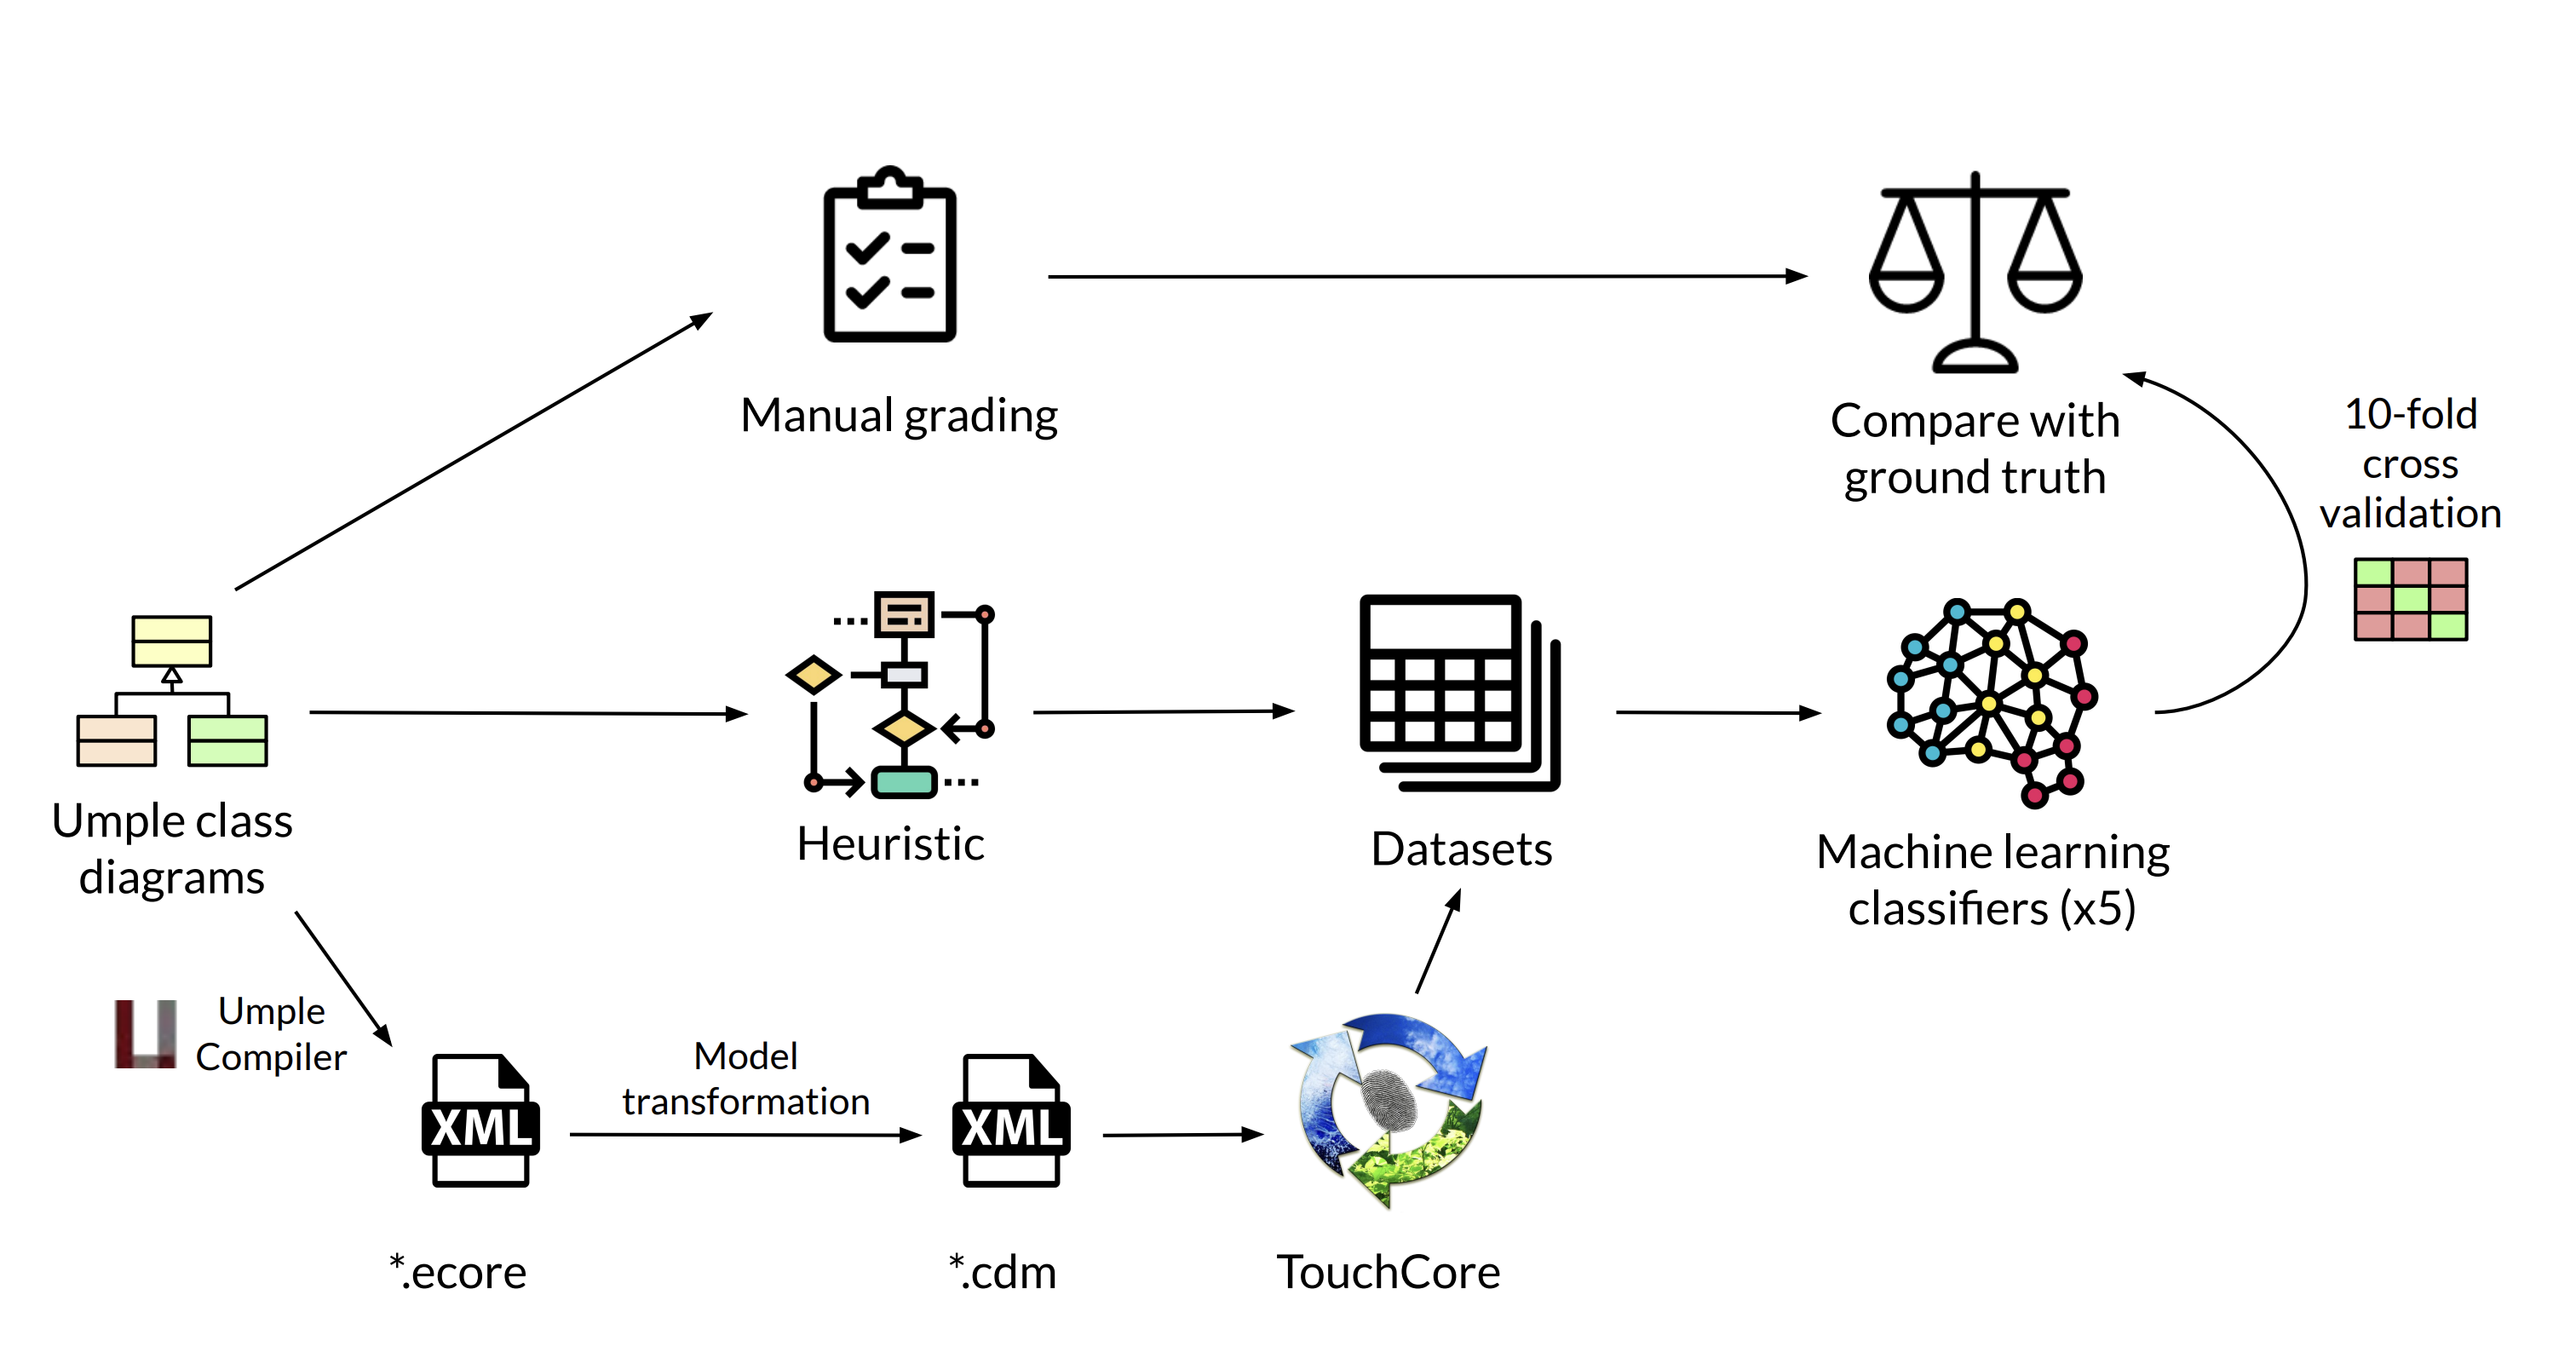
\includegraphics[width=13cm]{images/ml-approach}
	\caption{Ansatz der Studie \cite{boubekeur2020automatic}}
	\label{fig:ml-approach}
\end{figure}

Um die Effektivität ihres vorgeschlagenen Ansatzes zu validieren, führten die Autoren eine empirische Studie mit 50
Studierenden durch, die an einem Softwaretechnikkurs teilnahmen. Die Studierenden wurden gebeten, UML-Diagramme für ein
gegebenes Problem einzureichen, und die Autoren wandten ihren Ansatz zur Bewertung dieser Einreichungen an.
Um die Zuverlässigkeit der Bewertung sicherzustellen, wurden auch zwei menschliche Prüfer beauftragt, dieselben
Einreichungen unabhängig voneinander zu bewerten.

Die Ergebnisse der Studie zeigen, dass der vorgeschlagene Ansatz mit der menschlichen Bewertung hinsichtlich der
Identifizierung hochwertiger Einreichungen vergleichbar ist und erstaunlich präzise ungefähre Noten vorhersagen kann.
Darüber hinaus verglichen die Autoren ihren Ansatz mit einer komplexen regelbasierten Technik und stellten fest, dass
ihre Methode in Bezug auf Effizienz und Wartbarkeit überlegen ist~\cite{boubekeur2020automatic}. Diese Herangehensweise
weist jedoch einige zu berücksichtigende Schwächen auf:

\begin{enumerate}
    \item Es muss ein Zwischenmodell generiert werden, von dem aus die Diagramme der Studierenden bewertet werden,
    was zusätzliche Arbeit für die Lehrkräfte bedeutet~\cite{boubekeur2020automatic}.
    \item Die Herangehensweise funktioniert für allgemeine Diagrammfälle, aber ihre Effektivität nimmt ab, wenn die
    Modellierung komplexer wird~\cite{boubekeur2020automatic}.
    \item Die Autoren sprechen davon, dass die Herangehensweise mit einem begrenzten Datensatz getestet wurde und
    eine größere Menge an annotierten Daten benötigt, um sie zu verbessern, was für das
    Entwicklungsteam zeitintensiv sein kann~\cite{boubekeur2020automatic}.
    \item Das Trainieren und Evaluieren einer künstlichen Intelligenz ist eine mühsame Arbeit, die Jahre dauern kann~\cite{boubekeur2020automatic}.
\end{enumerate}

Die in dieser Masterarbeit behandelte Herangehensweise, wie sie im Konzeptkapitel~\ref{sec:konzept} dargelegt wird,
ermöglicht es hingegen, von einer bereits vorhandenen Musterlösung des Lehrers auszugehen, Regeln zu generieren und
Feedback zu erhalten, um einen Student schnell und ohne Zwischenkomplexität zu bewerten. Diese Musterlösung sollte im
Voraus annotiert werden, um zusätzliche Details hinzuzufügen, die zur Erstellung dieser Regeln erforderlich sind. Dieser
Ansatz ist schneller und erleichtert die Arbeit der Lehrkräfte.


\subsection{Bewertung auf Basis von Ähnlichkeitsmaßen}

Die Autoren des Artikels ``A Different Approach on Automated Use Case Diagram Semantic
Assessment''~\cite{fauzan2021different} sind Daniel Siahaan, Siti Rochimah, Reza Fauzan und Evi Triandini. Sie
untersuchten  einen semantischen Bewertungsansatz für Anwendungsfalldiagramme. Ihr Ansatz konzentriert sich auf
Eigenschaften und Beziehungen. Durch die Verwendung von Cosinus-Ähnlichkeit und WuPalmer für WordNet-Suchen bewerteten
sie 39 Diagramme ~\cite{fauzan2021different,al2017matching}, gesammelt aus drei Projekten.

Vor der Bewertung etablierten sie einen Goldstandard als Referenz basierend auf Expertenbewertungen von Studentenantworten. Die
vorgeschlagene Methode wurde mit dem Goldstandard verglichen, und die Ergebnisse zeigten eine hohe
Übereinstimmung. Interessanterweise war die Methode sogar präziser als die durchschnittliche Übereinstimmung zwischen
Experten~\cite{fauzan2021different}.

Die Autoren stellten fest, dass Lehrkräfte bei der Bewertung von Anwendungsfalldiagrammen tendenziell mehr Wert auf
Eigenschaften als auf Beziehungen legen. Dies könnte den Bewertungsprozess verbessern und zu einer objektiveren
Beurteilung führen. Die vorgestellte semantische Bewertung konzentriert sich auf die Bedeutung von Informationen in
Anwendungsfalldiagrammen und nicht nur auf ihre Form oder Struktur. Die Methode wurde jedoch noch nicht auf
Klassendiagramme übertragen, da diese eine andere Struktur haben. Diese Herangehensweise weist einige zu
berücksichtigende Schwächen auf:

\begin{enumerate}
    \item Diese Herangehensweise erfordert jedoch eine spezifischere Terminologie und Semantik seitens der Lehrkraft, was
    zusätzliche Anstrengungen von seiner Seite bedeutet.
    \item Diese Herangehensweise bedeutet, dass die Lehrkraft so präzise wie möglich sein muss, wenn er die Übung
    erstellt. Dadurch gibt er jedoch Anweisungen, die zu klar sind, was die Modellierungsaufgabe für den Studenten sehr
    offensichtlich macht.
    \item Diese Herangehensweise lässt der Vorstellungskraft des Studenten bezüglich der Modellierung keinen freien
    Raum, da die Anweisungen so präzise sind, dass es nur eine mögliche Lösung geben würde. Dies ist im Allgemeinen
    nicht der Fall bei Modellierungsaufgaben.
\end{enumerate}

Die Verwendung dieser Methode wäre daher nicht für das Hauptziel dieser Arbeit geeignet, das darin besteht, Lehrkräften
die Beurteilung von UML-Klassendiagrammen zu erleichtern.


\subsection{Graph matching zur Bewertung von UML}

Der Artikel mit dem Titel ``New method for summative evaluation of UML class diagrams based on graph similarities''
wurde von Outair Anas, Mohammed Ouadou und Abdelhadi Lotfi verfasst~\cite{anas2021new}. In ihrem Artikel widmen sich die
Autoren der Aufgabe der Bewertung von UML-Klassendiagrammen, die von Studierenden erstellt wurden. Sie
schlagen ein halbautomatisches System vor, das diese Aufgabe durch den Einsatz eines Vergleichs von syntaktischen,
strukturellen und semantischen Ähnlichkeiten angeht, um Fehler von Studierenden zu identifizieren und wertvolles
Feedback zu ihrem Lernprozess zu geben. Ihre Methode besteht aus drei Schritten:

\begin{enumerate}
    \item \textbf{UML-Diagramme in Graphen umwandeln:} Die Autoren beginnen ihren Ansatz, indem sie UML-Klassendiagramme
    in Graphdarstellungen umwandeln und das Metamodell durch die Einführung neuer Elemente zur Erleichterung der
    Bewertung verbessern. Sie stellen Klassen als Knoten dar, Attribute als mit Klassen verbundene Knoten und
    Assoziationen als beschriftete Kanten~\cite{auxepaules2015diagram}.

    \item \textbf{Definition von Ähnlichkeitsmaßen:} Die Autoren definieren eine Reihe von Ähnlichkeitsmaßen, die auf
    die transformierten UML-Graphen anwendbar sind. Sie untersuchen verschiedene Techniken zur Graphabstimmung und
    Metriken zur Knotenähnlichkeit, um den Vergleich von Graphen und die Fehlererkennung zu erleichtern~\cite{fauzan2018class}.

    \item \textbf{Abgleich und Vergleich von Graphen:} Unter Verwendung der zuvor definierten Ähnlichkeitsmaße führen
    die Autoren einen Abgleich und Vergleich der von Studierenden erstellten UML-Diagramme und der vom Lehrer
    bereitgestellten Referenzdiagramme durch~\cite{outair2017towards} (Siehe Abbildung~\ref{fig:graph-matching}).
\end{enumerate}


\begin{figure}
	\centering
	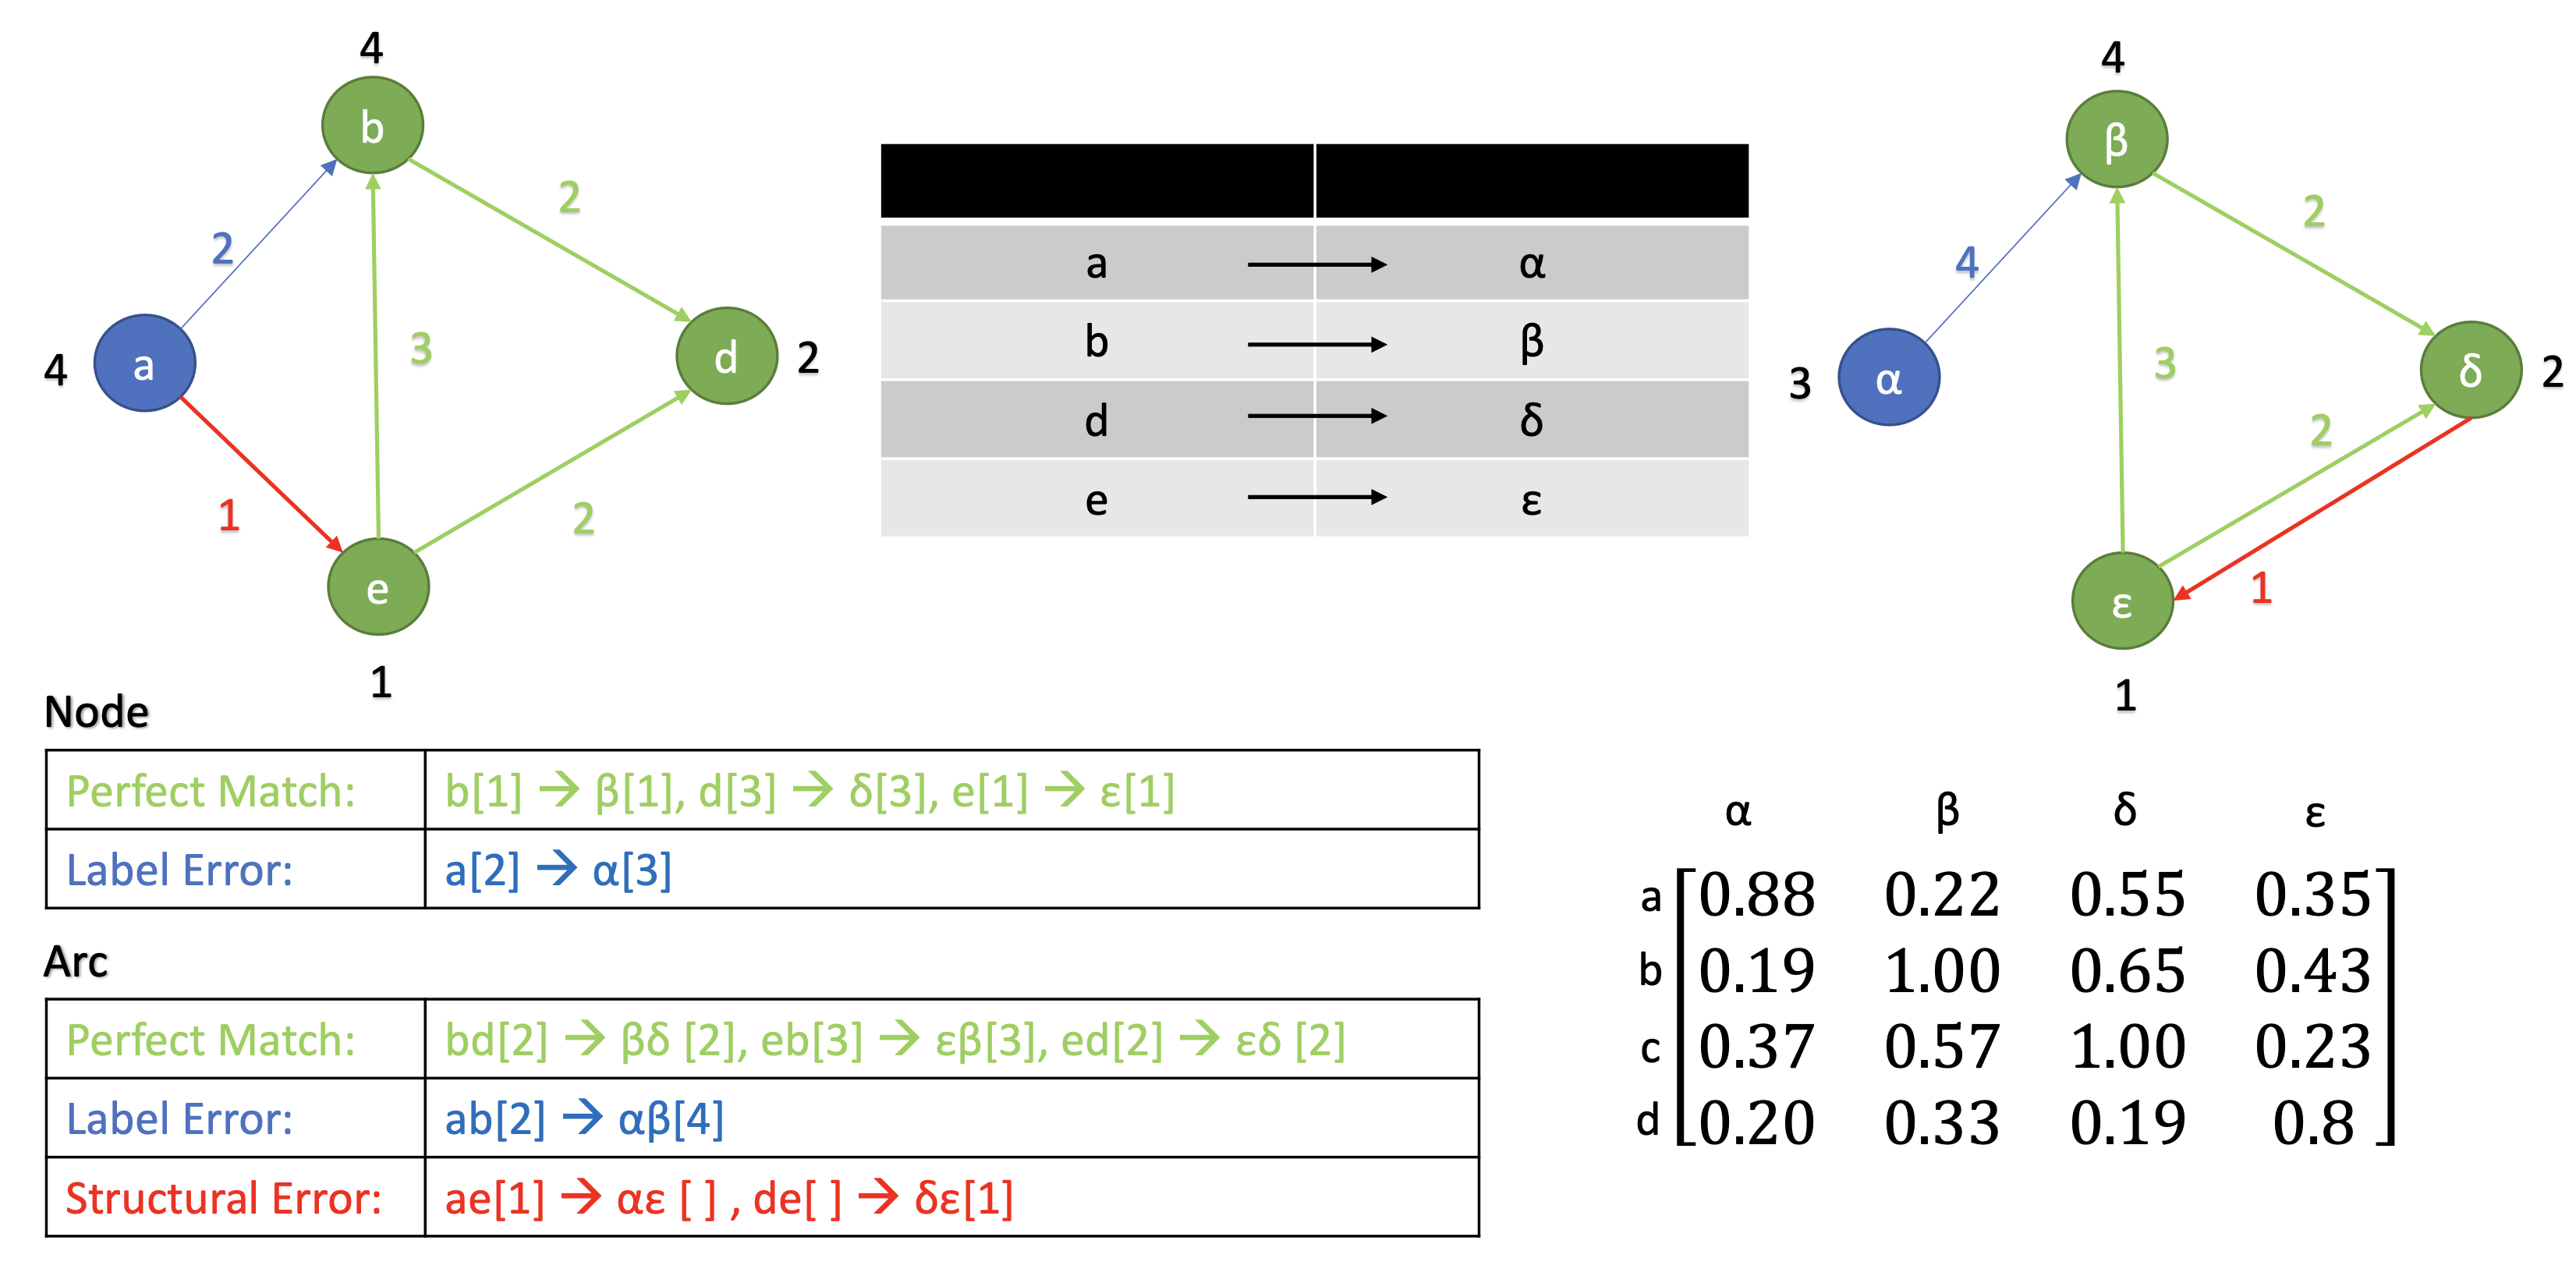
\includegraphics[width=13cm]{images/graph-matching}
	\caption{Beispiel für einen Graphenabgleich \cite{anas2021new}}
	\label{fig:graph-matching}
\end{figure}

Die Leistung des Systems wird anhand eines Datensatzes bewertet, der aus 100 von Studierenden erstellten
Klassendiagrammen besteht, wobei für jedes Diagramm ein entsprechendes Referenzdiagramm zur Bewertung bereitgestellt
wird. Drei Übungen wurden ausgewählt, um das System offline zu konfigurieren und zu bewerten, wobei iterative
Verbesserungen an den Ähnlichkeitskriterien und der Systemfunktionalität auf Grundlage der Übungsergebnisse vorgenommen
wurden. Die Ergebnisse zeigen, dass das System eine Genauigkeitsrate von 70 \% bei der Erkennung von Fehlern von
Studierenden erreicht und minimalen Eingriff erfordert, um Übereinstimmungen für 80 \% der verarbeiteten Diagramme zu
korrigieren~\cite{anas2021new}. Die Autoren betonen, dass der in das System integrierte formative Bewertungsansatz gut
geeignet ist, um UML-Klassendiagramme zu bewerten, da er den Studierenden Feedback zur Verbesserung ihres Verständnisses
des Lehrstoffes liefert. Darüber hinaus hat das System das Potenzial, die Belastung der Lehrenden zu verringern, indem
es den Bewertungsprozess automatisiert und ihnen ermöglicht, individuelleres Feedback an einzelne Studierende zu geben.
Dieser Ansatz weist einige zu berücksichtigende Schwächen auf:

\begin{enumerate}
    \item Die Autoren erkennen an, dass weitere Forschung erforderlich ist, um das System zu verfeinern und seine Genauigkeit zu
    verbessern.
    \item Dieser Ansatz ermöglicht keine Varianten oder Alternativen in den Lösungen, die die Studierenden präsentieren
    könnten. Sie konzentriert sich ausschließlich auf die Genauigkeit und lässt somit keinen Raum für mögliche
    Alternativen.
\end{enumerate}

Die in der Sektion zum Konzept~\ref{sec:konzept} vorgestellte Methode bietet eine direkte Lösung für dieses Problem.
Durch die Annotation der Lehrerlösung ist es möglich, verschiedene Modellierungsvarianten des Studierenden zu
berücksichtigen. Diese Methode ist zudem zuverlässiger, denn wenn das Modell und die Alternativen klar definiert sind,
liegt die Präzision stets bei 100\%.


\subsection{Automatisierte Bewertung mit GReQL}\label{subsec:automatisierte-bewertung-mit-greql}

In ihrem Artikel ``Automated checks on UML diagrams''~\cite{striewe2011automated} stellen Michael Striewe und Michael
Goedicke eine Technik zur Evaluierung von UML-Klassendiagrammen auf der Grundlage von Graphabfragen vor. Sie betrachten
UML-Klassendiagramme als Graphen und formalisieren ihren Ansatz mithilfe einer Graphabfragesprache namens GReQL.

\ac{GReQL}, ähnlich wie SQL, eignet sich gut für die Implementierung regelbasierter Prüfungen von graphenbasierten
Daten~\cite{striewe2014automated}. Sie ermöglicht die Abfrage von Elementen bestimmter Typen, die Untersuchung ihrer
Verbindungen und die Überprüfung ihrer Attribute. Im Kontext von UML-Klassendiagrammen können diese Abfragen das
Vorhandensein von Diagrammelementen wie Klassen, Schnittstellen, Eigenschaften, Operationen, Parametern, Assoziationen
und Generalisierungen ermitteln und ihre Beziehungen bewerten~\cite{striewe2011automated}.

\begin{lstlisting}[caption={[Codebeispiel] Codebeispiel in GReQL}, label={lst:greql}, float=!ht, language=xml]
  <rule type="presence" points="5">
    <query>
    from x : V{Class},
    y : V{Property}, z : V{PrimitiveType}
           with
              isDefined(x.name) and x.name="A" and
              x --> y and
              isDefined(y.name) and y.name="b" and
              y --> z and
              isDefined(z.name) and z.name="String"
           report 1 end
    </query>
    <feedback>Ein "A" soll ein Attribut für die
    Eigenschaft "b" bereitstellen.</feedback>
  </rule>
\end{lstlisting}

Um ein UML-Diagramm mithilfe dieses Ansatzes zu evaluieren, parsen die Autoren das Diagramm zunächst in eine
graphenbasierte Darstellung seiner abstrakten Syntax, in der Regel durch einen XML-Parser. Anschließend verwenden sie
\ac{GReQL}-Abfragen, um die Anwesenheit bestimmter Diagrammelemente und ihrer Verbindungen zu überprüfen. Die Autoren
stellen eine Reihe von Regeln vor, die als \ac{GReQL}-Abfragen implementiert sind und an die Anforderungen bestimmter
Kurse oder Aufgaben angepasst werden können.

In ihrem Bewertungssystem werden einzelnen Regeln individuelle Punktzahlen zugewiesen, wobei unterschiedliche
Gewichtungen zur Unterscheidung zwischen Korrektheits- und Qualitätsaspekten verwendet werden. Die Autoren schlagen auch
eine Methode zur Berechnung von Gesamtnoten vor, indem die Punktzahlen jeder Regel aggregiert werden~\cite{striewe2011automated}.

Diese Herangehensweise wurde für die Entwicklung des Konzepts verwendet (siehe Abschnitt~\ref{sec:konzept}). Durch sie
ist es möglich, ein Diagramm schnell zu bewerten und ein Feedback vom Lehrer zu erhalten. Im Vergleich zu anderen
Methoden ist diese Herangehensweise zuverlässiger und genauer hinsichtlich der erzielten Ergebnisse. Allerdings weist
sie auch mehrere Schwächen auf, die im Abschnitt zur Problemanalyse (siehe Kapitel~\ref{ch:problemanalyse}) dargelegt
werden. Eine Lösung zur Verbesserung des Bewertungsprozesses wird ebenfalls im Kapitel zum Konzept
(siehe Abschnitt~\ref{sec:konzept}) präsentiert.


\section{JACK}

Das E-Assessment-System namens ``JACK3'' (dritte Version von JACK)\cite{jack}, entwickelt von der Universität
Duisburg-Essen, stellt eine webbasierte Plattform dar, die Lehrkräfte eine effektive Lösung für die Erstellung und
Durchführung von Online-Übungen bietet. Diese vielseitige Plattform ermög-licht Lehrkräften die Erstellung einer breiten
Palette von Übungen, die nahtlos über eine benutzerfreundliche Oberfläche bereitgestellt werden können. Neben der
Erstellung von Bewertungen verfügt JACK3 über eine Auswahl an Funktionen, die den Bewertungsprozess optimieren sollen.
Diese beinhalten die automatisierte Bewertung, umfassende Berichterstellungswerkzeuge und die Echtzeitverfolgung des
Lernfortschritts der Schüler.

JACK3 bietet eine breite Palette von Übungstypen an, die den unterschiedlichen Lernzielen der Lehrkräfte und den
spezifischen Bedürfnissen ihrer Schüler gerecht werden. Zu den Beispielen gehören Multiple-Choice-Quizfragen,
Wahr/Falsch-Quizfragen, Zuordnungsübungen, Lückentext-übungen, Kurzantwortfragen Aufsatzfragen und vieles mehr. Des
Weiteren ermöglicht JACK3 die Erstellung komplexerer Übungen wie Drag-and-Drop-Aufgaben, Hotspot-Übungen, Umfragen zur
Datensammlung und Webquests, die eine tiefgehende Exploration von Themen ermöglichen~\cite{jack}.

Es ist erwähnenswert, dass JACK3 seine Fähigkeiten zur Unterstützung der Bewertung von Übungen zur Unified Modeling
Language (UML) erweitert hat, was seine Anwendbarkeit in der Softwaretechnik-Ausbildung verbessert. Lehrer können das
System nutzen, um UML-Diagramme wie Klassendiagramme, Sequenzdiagramme und Aktivitätsdiagramme automatisch zu bewerten.

Im Bereich der UML-Übungen bietet JACK3 Lehrern die Flexibilität, Übungen zu gestalten, die Klassendiagramme,
Sequenzdiagramme und Aktivitätsdiagramme umfassen. Diese Übungen ermöglichen es den Schülern, die Struktur und das
Verhalten von Softwaresystemen zu visualisieren, die komplexen Beziehungen zwischen Systemkomponenten zu verstehen,
ihre Ideen effektiv an Kommilitonen zu kommunizieren und ihre Fähigkeiten im Bereich Problemlösung und kritisches
Denken zu schärfen~\cite{jack}. JACK3 verwendet die im Abschnitt~\ref{subsec:automatisierte-bewertung-mit-greql}
vorgestellte Methode, um diese verschiedenen Diagrammtypen zu bewerten.


Das Hauptaugenmerk dieser wissenschaftlichen Arbeit liegt auf der Analyse und Evaluierung des Instrumentariums JACK,
insbesondere seiner Kapazität zur kritischen Beurteilung von UML-Diagrammen. Im darauf folgenden Abschnitt wird die
spezifische Problematik in umfassender Weise erörtert und eine breite Palette möglicher Lösungsansätze erörtert.
	\chapter{Problemanalyse}\label{ch:problemanalyse}

In diesem Kapitel erfolgt eine gründliche Analyse der zugrunde liegenden Problematik. Die Identifikation und eingehende Diskussion der spezifischen Herausforderungen und Schwierigkeiten, die im Rahmen dieser Arbeit behandelt werden, stehen dabei im Fokus.

\section{Beschreibung des Bewertungsprozesses}\label{sec:bewertungsprozess}
% Description de l'environnement

Wie bereits in den vorherigen Kapiteln erwähnt, verwendet die Fakultät für Informatik der Universität Duisburg-Essen (UDE) ein elektronisches Bewertungssystem namens ``JACK'' \cite{jack}, um bestimmte Prüfungen und Übungen automatisch zu bewerten. Unter den verschiedenen Arten von Übungen konzentriert sich diese Masterarbeit auf Übungen vom Typ UML.

Eine Übung vom Typ UML-Klassendiagramm besteht darin, die statische Struktur eines Software-Systems mithilfe der UML-Modellierungssprache zu modellieren \cite{reggio2013used}. Den Studierenden wird in der Regel eine Beschreibung des Systems, der wichtigsten Entitäten und ihrer Beziehungen zur Verfügung gestellt, und sie müssen dann ein Klassendiagramm erstellen, das diese Elemente darstellt. In diesem Diagramm sind die Klassen die Hauptobjekte, mit ihren Attributen (Variablen) und Methoden (Funktionen), und die Beziehungen zwischen den Klassen werden durch Assoziationen, Aggregationen oder Kompositionen dargestellt. Die Studierenden müssen besonders auf die Genauigkeit der Namen, Multiplizitäten und Kardinalitäten achten, um die Struktur des Systems korrekt widerzuspiegeln \cite{reggio2013used}. Das Hauptziel dieser Übung ist es, das Verständnis der objektorientierten Modellierungskonzepte zu vertiefen und eine solide Grundlage für die Softwareentwicklung zu schaffen. In Bezug auf das JACK-System kann der Bewertungsprozess in mehrere verschiedene Phasen unterteilt werden:

\vspace{0.5cm}

\textbf{Phase 1: Erstellung der Übung}

In dieser ersten Phase erstellt der Lehrer die Übung, indem er eine schriftliche Beschreibung eines zu modellierenden Systems bereitstellt. Besonderes Augenmerk wird auf die Genauigkeit der Bezeichnungen der Entitäten und die Klarheit und Explizitheit der Beziehungen zwischen ihnen gelegt. Der Lehrer hat dann einen Bereich in der JACK-Anwendung, in den er diesen Text einfügen kann, der von den Studierenden eingesehen wird.

\\~\\
\textbf{Phase 2: Erstellung einer Musterlösung oder Anmerkung (optional)}

In dieser Phase kann der Lehrer entscheiden, ein UML-Diagramm als Musterlösung für die Übung zu erstellen. Dies erleichtert das Verständnis der Übung, ermöglicht die Überprüfung der Kohärenz und Durchführbarkeit des Systems. Alternativ kann der Lehrer die Übung lediglich annotieren, um die Schlüsselbegriffe und -elemente hervorzuheben, die in der späteren Phase nützlich sein werden.

\\~\\
\textbf{Phase 3: Entwicklung des GReQL-Codes}

In dieser Phase verwendet der Lehrer seine Anmerkungen und die Musterlösung, um den GReQL-Code zu entwickeln, der von
JACK interpretiert wird, um die von den Studierenden eingereichten Lösungen zu bewerten. JACK verwendet den GReQL-Code
sowie verschiedene in dieser Sprache definierte Regeln, um die UML-Diagramme zu bewerten. Zusätzlich zum GReQL-Code wird
vom Lehrenden auch ein Feedbacktext sowie die mit jeder Regel verbundenen Gewichtungen bereitgestellt. Alle diese
verschiedenen Informationen werden in einem XML-Format verfasst, das auf JACK hochgeladen wird. Wenn ein Student seine
Lösung einreicht, wird eine grafische Darstellung dieser Lösung erstellt, und der GReQL-Code führt Abfragen auf dieser
Darstellung aus, um eine Bewertung für die Lösung des Studenten zu vergeben~\cite{striewe2011automated}.

\\~\\
\textbf{Phase 4: Einreichung der Lösung durch den Studenten}

Nachdem der Student an der Lösung der Übung gearbeitet hat, lädt er ein XML-Dokument im XMI Format auf JACK hoch. Zur Generierung dieses kompatiblen XMI-Dokuments verwenden Studierende Tools wie BOUML \cite{bouml} oder Software Ideas Modeler \cite{sim}, mit denen sie XMI-Code aus einer zuvor erstellten grafischen UML Darstellung ableiten können. Dieses Dokument repräsentiert die von ihm entwickelte Lösung.

\\~\\
\textbf{Phase 5: Bewertung des Diagramms}

Das von den Studierenden eingereichte Diagramm wird anhand des von den Lehrern verfassten GReQL-Codes bewertet. Anschließend wird dem Studenten ein Feedback zugeteilt.


Diese Phasen veranschaulichen die grundlegende Funktionsweise der JACK-Plattform in Bezug auf die automatisierte Bewertung von Übungen zur Erstellung von UML-Klassendiagrammen.


\section{Untersuchung des Problems}

Im Verlauf der dritten Phase, wie im vorherigen Kapitel beschrieben, sehen sich Lehrende mit der Notwendigkeit konfrontiert, GReQL-Code zu verfassen, der vom JACK-System zur Bewertung der Einreichungen verschiedener Studierender verwendet wird. Diese Phase stellt jedoch bereits auf verschiedenen Ebenen eine Herausforderung für die Lehrenden dar, aus folgenden Gründen:

\vspace{0.5cm}

\textbf{Erforderliche Expertise für die Erstellung von GReQL-Code:}
Das Verfassen von GReQL-Code erfordert eine gewisse Expertise. Auf den ersten Blick mag die Syntax von GReQL nicht schwer zu verstehen sein. Dennoch kann es anspruchsvoll sein, die Feinheiten der Code-Erstellung zu beherrschen. Dies erfordert von den Lehrenden mehrere Stunden, intensives Üben und umfangreiche Tests, um einen Code zu erstellen, der präzise bewertet, insbesondere in Fällen von komplexeren Beziehungen zwischen Entitäten.

\vspace{0.5cm}

\textbf{Hohe Möglichkeit von Fehlern im GReQL-Code:}
Selbst bei Beherrschung der Feinheiten von GReQL sind Lehrende nicht vor möglichen Fehlern gefeit. Diese Fehler können zwar geringfügig erscheinen, haben jedoch das Potenzial, das Bewertungssystem erheblich zu beeinträchtigen.

\vspace{0.5cm}

\textbf{Zeitaufwand für die Erstellung von GReQL-Code:}
Die Bewertung jedes Diagramms erfordert erheblichen Zeitaufwand, um einen GReQL-Bewertungscode zu erstellen,
insbesondere für komplexere Beziehungen zwischen verschiedenen Entitäten.

\vspace{0.5cm}

\textbf{Wartung und Anpassungsfähigkeit des GReQL-Codes:}
Nachdem der GReQL-Code erstellt und für die Bewertung von UML-Diagrammen implementiert wurde, kann eine kontinuierliche
Wartung erforderlich sein. Mit steigenden Anforderungen an die Bewertung kann es sein, dass der GReQL-Code regelmäßig
aktualisiert und angepasst wird. Dies stellt für Lehrende eine fortwährende Herausforderung dar und erfordert Zeit und
Aufwand, um sicherzustellen, dass das Bewertungssystem präzise und relevant bleibt.

\vspace{0.5cm}
\textbf{Bedarf an Ressourcen und technischer Unterstützung:}
Lehrende benötigen möglicherweise Zugang zu technischen Ressourcen und angemessener Unterstützung, um die Kunst der effizienten GReQL-Code-Erstellung zu beherrschen. Dies kann Schulungen, Orientierungsdokumente, Diskussionsforen oder andere Formen technischer Unterstützung einschließen. Die Beschaffung dieser Ressourcen kann Zeit in Anspruch nehmen und eine institutionelle Koordination erfordern.

\vspace{0.5cm}
Dies sind die verschiedenen Herausforderungen, die bei der Erstellung von GReQL-Code für die Bewertung von UML-Diagrammen auf der JACK-Plattform auftreten können.


\section{Ableitung und Abgrenzung der Anforderungen}
% Description des choses à faire ainsi qu'une limitation


Das Ziel dieser Masterarbeit ist nicht, Lehrkräfte von der Notwendigkeit zu befreien, GReQL-Code zu schreiben, zu
bearbeiten oder zu ändern. Dies ist auf die quasi unendliche Vielfalt an Möglichkeiten zurückzuführen, wenn es darum
geht, GReQL-Code zu verfassen, und darauf, dass es für ein Werkzeug unmöglich ist, diese Aufgabe perfekt zu erfüllen
und alle möglichen Optionen und Alternativen ohne menschliches Eingreifen abzudecken. Vielmehr geht es darum, den
Prozess der Regeldefinition erheblich zu erleichtern, indem Lehrkräfte in diesem Generierungsprozess von Regeln
unterstützt werden. Auf diese Weise können sich Lehrkräfte auf weniger triviale Aufgaben konzentrieren. Um diesen Prozess
zu vereinfachen, zielt diese Masterarbeit darauf ab, ein Verfahren zu entwickeln und in Form einer Softwareanwendung zu
prototypisieren, mit dem (halb-)automatisch Bewertungsregeln aus annotierten Musterlösungen erstellt werden können.
Bei der Erstellung von Übungen für UML erstellen Lehrkräfte in den meisten Fällen eine spezifische Musterlösung für
diese Übungen. Ausgehend von den bereits vorhandenen Musterlösungen wäre deren Annotierung ein äußerst interessanter
Ausgangspunkt, da keine zusätzliche Ressource für Lehrkräfte erforderlich ist. Basierend auf diesem spezifischen
Kriterium wurde die Entscheidung zur Annahme dieses Ansatzes in Betracht gezogen, um das System zu entwickeln. Dieses
System soll in der Lage sein, folgende Ziele zu erreichen:

\begin{enumerate}[itemsep=8pt, parsep=5pt]
    \item \textbf{Verminderung der Einstiegshürde:} Es strebt danach, den Prozess der Erstellung von GReQL-Regeln zu erleichtern. Selbst jemand, der keine Vorkenntnisse in GReQL hat, sollte unser Tool verwenden können, um Regeln zu erstellen, die bereits eine Bewertung von einfachen Diagrammen und Beziehungen ermöglichen.
    
    \item \textbf{Verbesserung der Präzision und Zuverlässigkeit der GReQL-Regeln:}
    Durch die Nutzung von annotierten Musterlösungen zielt die Anwendung darauf ab, die Präzision und Zuverlässigkeit der generierten Regeln zu verbessern. Dies würde das Risiko von Fehlern und Inkonsistenzen in den Bewertungsregeln verringern und somit eine konsistentere Bewertung der studentischen Arbeiten gewährleisten.
    
    \item \textbf{Verbesserung des Zeit- und Arbeitsaufwands der Lehrkräfte:}
    Durch Automatisierung eines Teils des Regelbildungsprozesses zielt das System darauf ab, Zeit und Aufwand der Lehrkräfte zu sparen. Dies würde es ihnen ermöglichen, sich mehr auf das Lehren und Betreuen der Studierenden zu konzentrieren, anstatt auf mühsame administrative Aufgaben.
    
    \item \textbf{Förderung der Skalierbarkeit und Wartbarkeit der Regeln:}
    Durch die Implementierung eines Mechanismus zur Pflege und Aktualisierung der generierten Regeln würde die Anwendung dazu beitragen sicherzustellen, dass die Regeln relevant und anpassungsfähig bleiben und sich den sich ändernden Anforderungen von Lehre und Bewertung anpassen.
    
    \item \textbf{Unterstützung einer breiten Palette von Bewertungsszenarien:}
    Die Anwendung sollte flexibel genug sein, um eine Vielzahl von Bewertungsszenarien zu unterstützen, einschließlich solcher mit komplexen Diagrammen und Beziehungen. Dadurch würde sie eine vielseitige Lösung für Lehrkräfte bieten.
    
\end{enumerate}

Das Ziel dieser Initiative ist es, den Prozess der Bewertung von UML-Diagrammen effizienter, zugänglicher und präziser zu gestalten, während die administrativen Arbeitslasten der Lehrkräfte reduziert werden. Dadurch soll die Qualität von Lehre und Bewertung im Bereich der Softwaremodellierung verbessert werden.

	\chapter{Entwicklung des Konzepts}

In diesem Kapitel wird der Übergang von der Problemanalyse zur kreativen Konzeptentwicklung im Forschungsprozess betont.
Es wird die zentrale Phase markiert, in der theoretisches Wissen und praktische Erkenntnisse zusammengeführt werden, um
innovative Lösungsansätze zu formulieren. Theoretische Grundlagen und Modelle aus vorangegangenen Kapiteln werden
integriert und die angewandten Methoden zur Entwicklung tragfähiger Lösungen werden erläutert. Dieses Kapitel wird als
Brücke zwischen Analyse und Umsetzung genutzt, wobei die kreative Synthese von Ideen und Lösungsansätzen betont wird.
Ein detaillierter Einblick in den Prozess der Konzeptentwicklung wird geboten.

\section{Verschiedene Herangehensweisen}

Vor der Ausarbeitung des endgültigen Implementierungskonzepts wurden mehrere methodische Ansätze im Detail untersucht.
Das Hauptziel dieser methodischen Ansätze bestand darin, eine Reihe von Regeln zu extrahieren, die anschließend in
GReQL-Ausdrücke umgewandelt werden sollten. Diese Regelsets sollten aus den Kommentaren oder Notizen extrahiert werden,
die von den Lehrkräften zu einer UML-Übung hinterlassen wurden. Die Wahl des Notizformats ist offen, was viele
Möglichkeiten bietet. Zwei Ansätze, die in diesem Rahmen erkundet wurden, werden in diesem Kapitel vorgestellt.

\subsection{YAML-basierten Annotationen}

Der erste untersuchte methodische Ansatz fokussierte auf die Entwicklung eines benutzerfreundlichen Annotationsystems, das eine umfassende Modellierung der Interaktionen innerhalb eines UML-Diagramms ermöglichen sollte. Infolgedessen wurden editierbare Regelobjekte abgeleitet, welche aus diesem Annotationsystem generiert wurden. Sobald der Nutzer sämtliche Regeln, die aus dem Annotationsystem resultierten, verifizierte, konnte er GReQL-Code generieren, welcher anschließend in das JACK-System eingefügt wurde. Die Konzeption dieses schlichten Notationssystems diente dem Zweck der Abbildung von Beziehungen innerhalb eines UML Klassendiagramms. Zu diesem Zweck wurde das YAML-Format aus mehreren Gründen präferiert:

\begin{enumerate}
    \item Erstens, das Schreiben im YAML-Format erweist sich als unkompliziert.
    \item Zweitens, es liefert Daten in einem strukturierten Format, welches leicht manipuliert werden kann.
\end{enumerate}


\begin{figure}
	\centering
	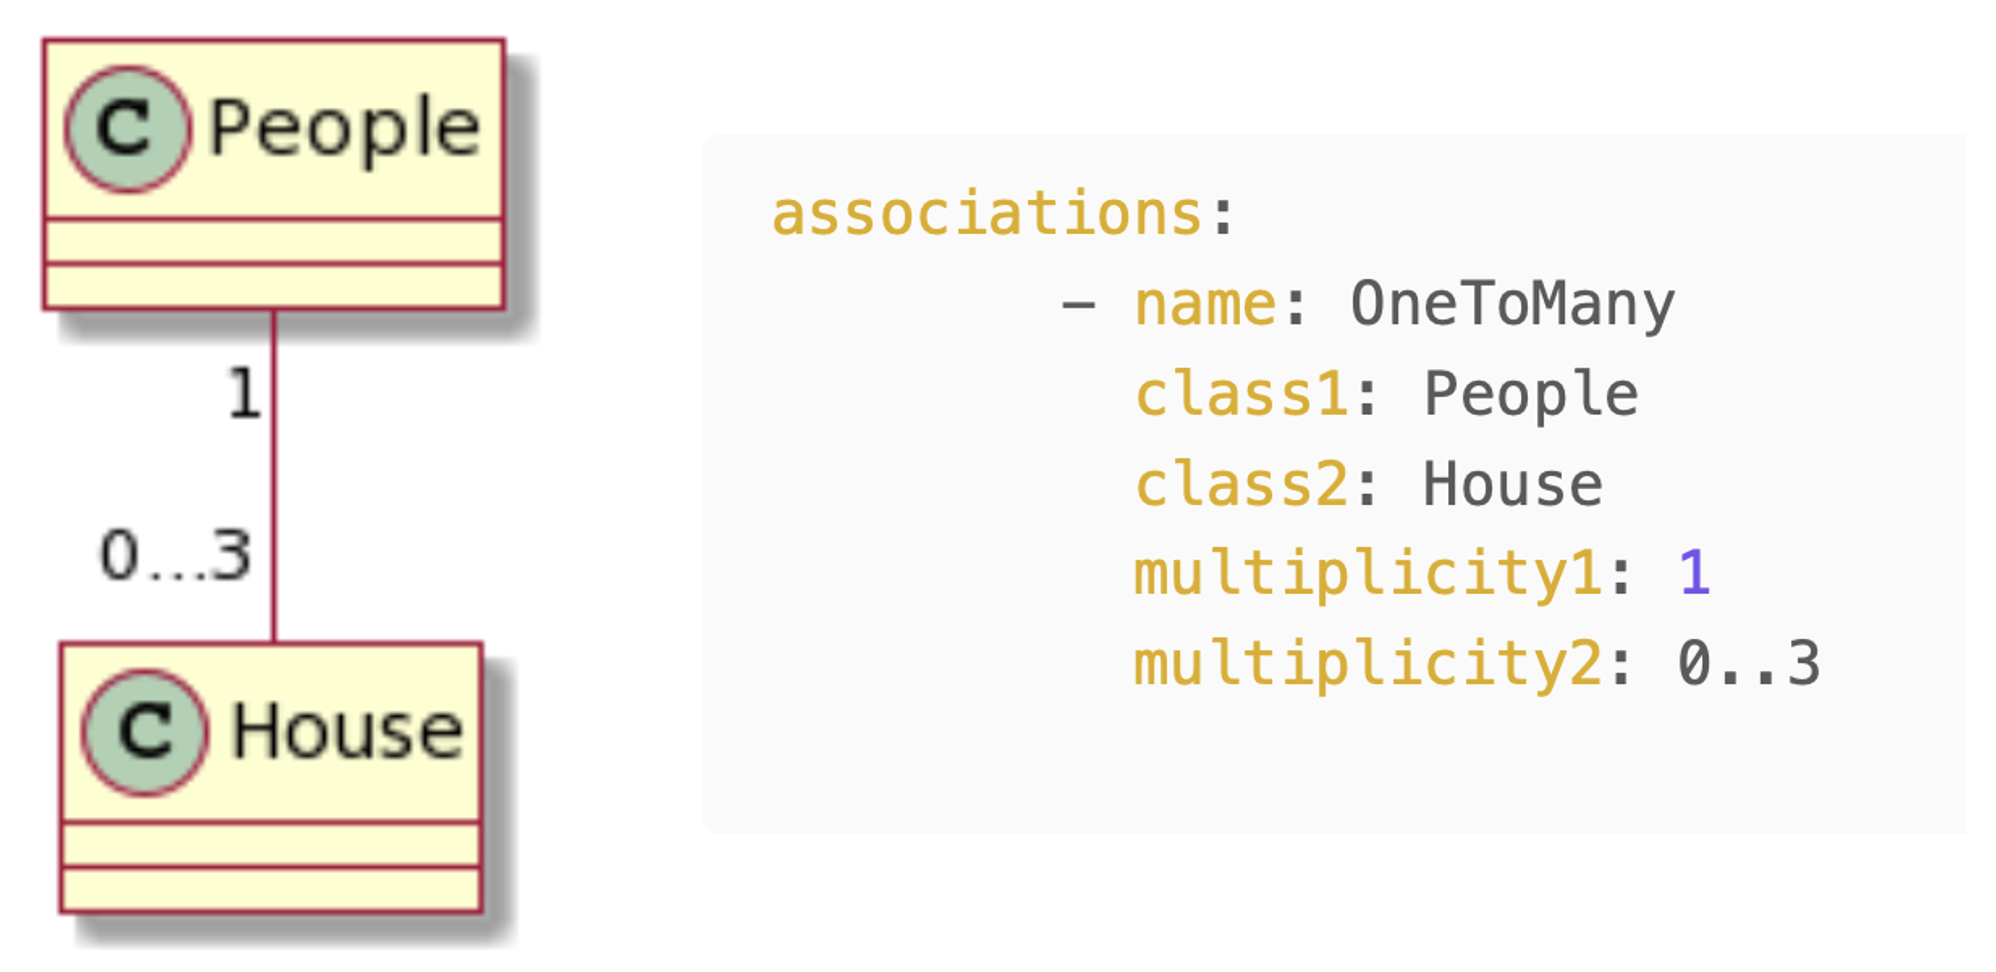
\includegraphics[width=10cm]{images/yaml-uml}
	\caption{Beispiel einer Annotation von UML mit YAML}
	\label{fig:yaml-uml}
\end{figure}


Die Notation in YAML mag den Eindruck vermitteln, bereits eine Form der Regeldefinition darzustellen, weil der Lehrende bereits alle Interaktionen zwischen den verschiedenen Objekten im Diagramm definiert. Um jedoch die Klarheit bezüglich dieser Frage zu gewährleisten, könnte es sinnvoll sein, ein weniger formelles Notationssystem zu etablieren. Beispielweise:

\begin{itemize}
    \item Die Klasse A erbt von der Klasse B.
    \item Die Klasse A besitzt drei Attribute:
    \begin{itemize}
        \item Attribut a vom Typ x mit öffentlicher Sichtbarkeit.
        \item Attribut b vom Typ y mit öffentlicher Sichtbarkeit.
        \item Attribut c vom Typ z mit privater Sichtbarkeit.
    \end{itemize}
\end{itemize}

oder ein noch weniger wortreiches System: 

\begin{itemize}
    \item A $\Rightarrow$ B 
    \item A:
    \begin{itemize}
        \item +a:x (+ für öffentlich)
        \item +b:y
        \item -c:z (- für privat)
    \end{itemize}
\end{itemize}


Dieses System ähnelt eher herkömmlichen Kommentaren, jedoch könnte es herausfordernder sein, den darin enthaltenen Text zu analysieren und daraus anwendbare Regelvorschläge zu extrahieren. Trotzdem birgt dieser methodische Ansatz mehrere Limitationen:

\begin{enumerate}
    \item Es existieren bereits seit geraumer Zeit vielfältige Notationssysteme und Datenformate für UML, wie beispielsweise XMI \cite{skogan1999uml}, \ac{UXF} \cite{suzuki1998making}, Textbasierte \cite{washizaki2010tcd} oder JSON-basierte Datenformate \cite{benson2021uml}, um nur einige zu nennen.

    \item Die Entwicklung eines vollständig neuen und umfassenden Notationssystems innerhalb eines begrenzten Zeitraums kann äußerst zeitintensiv sein, insbesondere wenn es die umfassende Darstellung sämtlicher Varianten eines UML-Klassendiagramms anstrebt.

    \item Dieses System verlagert die Aufgabe der Ableitung von Beziehungen zwischen den verschiedenen Objekten lediglich in ein anderes Format, ohne dabei die Arbeitsbelastung für die Lehrkraft zu mindern.
\end{enumerate}


In Anbetracht dieser diversen Überlegungen wurde von der Verfolgung dieses methodischen Ansatzes Abstand genommen, und es erfolgte die Exploration alternativer Vorgehensweisen.


\subsection{Verwendung von Natural Language Processing  Tools}

Die zweite konzeptionelle Idee besteht darin, ein \ac{NLP}-Tool zu verwenden, um die Kommentare oder Notizen des Lehrers zu analysieren. Anschließend kann das NLP-Tool verwendet werden, um Empfehlungen auf der Grundlage einer vorher festgelegten Reihe von Parametern für den Lehrer abzugeben. Diese Parameter könnten eine Reihe von UML-Regeln in einem spezifischen Format sein, so dass die KI in der Lage ist, die richtige Lösung auf der Grundlage des Kommentars zu finden. Der Vorschlag könnte dann in GReQL-Code übersetzt werden. Diese Herangehensweise hat jedoch auch einige Herausforderungen:

\begin{enumerate}
    \item Die von dieser Methode generierten Lösungen neigen dazu, ungenau zu sein, und es sind möglicherweise zahlreiche Anpassungen erforderlich, um das gewünschte Ergebnis zu erzielen \cite{chowdhary2020natural}. Dies könnte möglicherweise die Arbeitsbelastung der Lernenden erhöhen, anstatt sie zu erleichtern.
    \item Es wäre notwendig, die KI darauf zu trainieren, bestimmte Muster zu erkennen und sie mit vordefinierten Regeln in Verbindung zu bringen, um die Zuverlässigkeit zu erhöhen.

\end{enumerate}

In ihrem aktuellen Stand erfordert diese Herangehensweise erhebliche Anstrengungen, um diese Herausforderungen zu bewältigen und eine effektive Implementierung zu erreichen. Aufgrund der potenziellen Schwierigkeiten bei der Implementierung und der möglicherweise nicht zufriedenstellenden Ergebnisse wurde dieser Ansatz auch aufgegeben.

\section{Konzept}\label{sec:konzept}

Bei der Entwicklung des Konzepts wurde ein andersartiger Ansatz als der in dem vorherigen Abschnitt dargelegte verfolgt. Die Herangehensweise, Regeln aus Kommentaren abzuleiten, erweist sich als ein komplexer Prozess und potenziell schwierig umzusetzen. Die Gewährleistung der Zuverlässigkeit der erzielten Ergebnisse stellt ebenfalls eine bedeutende Herausforderung dar. In diesem Zusammenhang wurde eine intuitivere Herangehensweise in Betracht gezogen, nämlich die direkte Ableitung von Regeln aus der Mustervorlage.

Bevor dieses Konzept im Detail beschrieben wird, ist es unerlässlich, das Endziel in Erinnerung zu rufen, nämlich die Unterstützung von Lehrenden bei der Bewertung von UML-Übungsaufgaben (insbesondere Klassendiagrammen). Dies soll durch erhebliche Vereinfachung des Schreibens von GReQL-Code auf der JACK-Plattform erreicht werden, indem Lehrern mit Hilfe eines im Rahmen dieser Masterarbeit zu entwickelnden Tools (halb-)automatische Unterstützung geboten wird. Das Konzept zur Erfüllung dieser Aufgabe kann in drei Wichtige Schritte unterteilt werden:

\subsubsection{Schritt 1: Erstellung einer Musterlösung mit Hilfe eines Modellierungstools}

Wie im \autoref{sec:bewertungsprozess} erwähnt wurde, umfasst Phase 2 die optionalen Schritte zur Erstellung einer Musterlösung. In diesem Konzept ist diese Phase unerlässlich und gewinnt ihre volle Bedeutung. Nachdem ein UML-Klassendiagrammübungsaufgabe entwickelt wurde, erstellen die meisten Lehrer eine Musterlösung, oft in Form eines Klassendiagramms. Diese Lösung wird dann mit den verschiedenen Einreichungen der Studenten verglichen, und Punkte werden gemäß den vom Lehrer festgelegten Kriterien an die einzelnen Studenten vergeben. Da in den meisten Fällen eine Musterlösung in Form eines Klassendiagramms für die Aufgabe vorhanden ist, wäre es sinnvoll, diese zur Ableitung relevanter Regeln zu verwenden. Dies stellt die erste Phase des Ansatzes dar, bei der eine Musterlösung mithilfe einer Modellierungsanwendung erstellt wird, die anschließend die Möglichkeit bietet, das Diagramm in einem leicht programmierbaren Format zu exportieren.

\subsubsection{Schritt 2: Verarbeitung der exportierten Datei}

Nachdem der Lehrer die Musterlösung erfolgreich modelliert hat, ergibt sich die Notwendigkeit, diese Vorlage in ein geeignetes Format zu exportieren, welches eine programmgesteuerte Bearbeitung ermöglicht. Dieser Transformationsprozess kann mittels diverser Datenformate wie JSON, XML oder sogar YAML realisiert werden. Sobald das exportierte Dokument verfügbar ist, eröffnet sich im Kontext eines Klassendiagramms die Möglichkeit, zunächst sämtliche in der Musterlösung enthaltenen Klassen sowie sämtliche Interdependenzen zwischen den verschiedenen Elementen zu extrahieren. Infolge dieses Phasenschritts besteht die Option zur Ableitung von ``Regel''-Objekten, welche auf der Frontend-Oberfläche sichtbar sind und vom Lehrer interaktiv bearbeitet werden können. Die Integration dieser Funktionalität ermöglicht Lehrkräften, wertvolles Feedback und alle zugehörigen Informationen durch eine einzige Annotation hinzuzufügen, um sowohl die Punktzahlen festzulegen als auch den nächsten Schritt und die anschließende Evaluierung umfassend zu unterstützen.

\subsubsection{Schritt 3: Generierung des GReQL-Codes}

Der abschließende Schritt dieses Vorgehens umfasst die Generierung von GReQL-Code aus den Regeln, die in der vorherigen Phase extrahiert und/oder hinzugefügt wurden. Nachdem die Konfiguration abgeschlossen ist, muss der GReQL-Code unter Verwendung verschiedener XMI-Vorlagen generiert werden. Der resultierende Code kann vom Lehrer auf der JACK-Plattform verwendet werden.

\begin{figure}
	\centering
	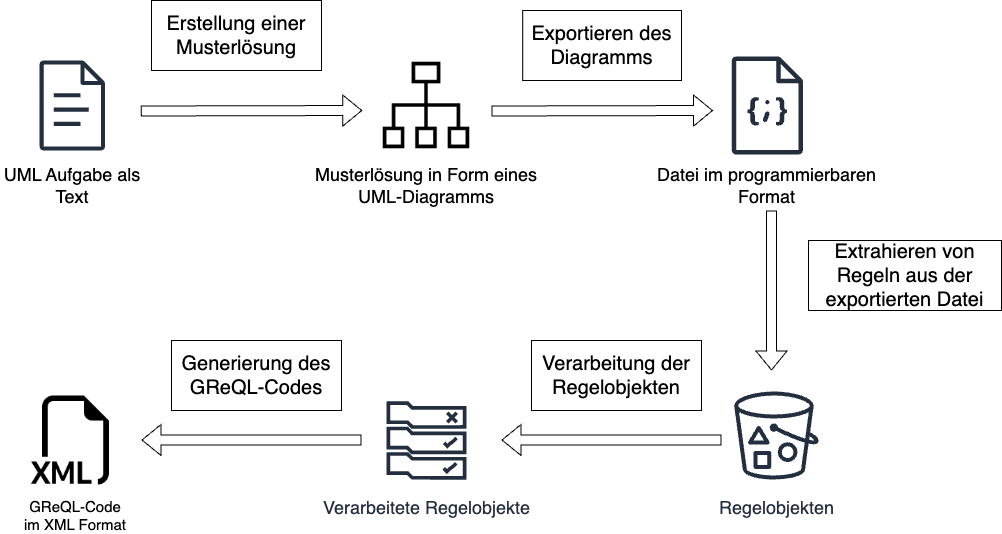
\includegraphics[width=13cm]{images/concept}
	\caption{Repräsentatives schema des konzepts}
	\label{fig:concept}
\end{figure}

Durch dieses Konzept und seine verschiedenen Schritte ist es möglich, von einer Musterlösung zur Generierung des erforderlichen GReQL-Codes für die Bewertung von Diagrammen durch JACK zu gelangen. Dieser Ansatz hat das Potenzial, den Bewertungsprozess von Diagrammen über die JACK-Plattform erheblich zu vereinfachen, was das zentrale Ziel dieser Masterarbeit ist. Die tatsächliche Umsetzung dieses Konzepts hängt jedoch eng vom gewählten Workflow und der Art und Weise ab, wie das Konzept umgesetzt wird. Dieser Ausblick leitet zum nächsten Kapitel über, das die Implementierung behandelt.
	\chapter{Implementierung}

Das vorliegende Kapitel widmet sich der umfassenden Dokumentation des Implementierungsprozesses des zuvor beschriebenen
Konzepts. Es bietet eine detaillierte Aufarbeitung der technischen Umsetzung und des Entwicklungsprozesses, der im
Rahmen dieser Masterarbeit durchgeführt wurde. Beginnend mit einer umfassenden Beschreibung der verwendeten Technologien
und Werkzeuge sowie einer ausführlichen Begründung für die Wahl dieser spezifischen Technologien, wird dieses Kapitel
einen tiefen Einblick in die präzise Umsetzung des Konzepts gewähren. Die Implementierung ist ein entscheidender Schritt
zur Realisierung des in den vorherigen Kapiteln skizzierten Ansatzes zur Bewertung von UML-Diagrammen. Durch die
Dokumentation dieses Schrittes wird das Verständnis für die technischen Aspekte des Projekts vertieft und ermöglicht
eine transparente Darstellung des Entwicklungsprozesses.

\section{Überblick über angewendete Werkzeuge und Technologien}
Dieses Kapitel konzentriert sich auf die Vorstellung der Werkzeuge, die für die Umsetzung des im vorherigen Kapitel
vorgestellten Konzepts verwendet werden. Es wird jedes Werkzeug vorgestellt und die Auswahl begründet.

\subsection{PlantText}

Der erste Schritt des im vorherigen Kapitel vorgestellten Konzepts besteht in der Modellierung eines UML-Diagramms.
Diese Modellierungsphase verlangt die Anwendung einer Software-Anwendung, welche in der Lage ist, das entworfene
Diagramm in ein Format zu überführen, welches für die anschließende Extraktion der enthaltenen Regelsätze dienlich
ist. Eine facettenreiche Auswahl an digitalen Werkzeugen steht zur Verfügung, um diese spezifische Aufgabe zu
bewältigen, wobei PlanText exemplarisch zu nennen ist.

PlantText~\cite{planttext} ist ein webbasiertes Instrument zur Diagrammmodellierung, das insbesondere in den Domänen
der UML und anderer Modellierungssprachen einen renommierten Status innehat. Dieses Instrument wurde entwickelt,
um die bequeme Erstellung, Bearbeitung und gemeinsame Nutzung von Diagrammen in einer kollaborativen Umgebung zu
ermöglichen. Seine Auszeichnungen resultieren aus der Benutzerfreundlichkeit, der Flexibilität und der
Leistungsfähigkeit, wodurch es zu einer favorisierten Wahl für Softwareentwickler, Systemarchitekten und Projektmanager
avanciert~\cite{planttext}.

PlantText basiert auf einer schlichten, aber wirkungsvollen Konzeption, nämlich der Generierung von Diagrammen durch
Verwendung von textuellen Notationen. Benutzer können Diagramme unter Einsatz von natürlicher Sprache und vordefinierten
Schlüsselwörtern kreieren, wodurch der gesamte Prozess simplifiziert wird. Eine prototypische Darstellung einer Klasse
in einem UML-Klassendiagramm kann etwa wie folgt aussehen:


\begin{lstlisting}[caption={[Codebeispiel] PlantText code Example}, label={lst:Planttext}, float=!ht, language=javascript]
class A {
   + attribute1: Typ1
   - attribute2: Typ2
   # operation1(): void
}
\end{lstlisting}

In diesem Illustrationsfall repräsentieren einfache Textnotationen die Klasse ``A'', ihre Attribute und Methoden.
Die Verwendung von ``+'' für öffentliche Attribute, ``-'' für private Attribute und ``#'' für Methoden gestaltet sich
intuitionsgetreu und erleichtert die Entwicklung von UML-Diagrammen erheblich. PlantText beinhaltet eine leistungsstarke
Rendering-Engine, die diese textlichen Notationen automatisiert in visuell ansprechende Diagramme konvertiert. Benutzer
sind in der Lage, die Diagramme in Echtzeit zu visualisieren und zu editieren, ohne sich mit den komplexen Details der
grafischen Gestaltung auseinandersetzen zu müssen. Diese textorientierte Herangehensweise führt zu einer höchst
effizienten und adaptierbaren Gestaltung und Veränderung von Diagrammen. Die Vorzüge der Anwendung von PlantText
manifestieren sich unter anderem in:

\begin{enumerate}
    \item \textbf{Benutzerfreundlichkeit:} PlantText ist für Einsteiger und erfahrene Modellierer gleichermaßen zugänglich.
Die Verwendung von textuellen Notationen vereinfacht den Einstieg und reduziert die Lernkurve, da sie natürlicher und
verständlicher sind als grafische Schnittstellen~\cite{mazanec2012general}.
    \item \textbf{Kollaboration und gemeinsame Nutzung:} PlantText bietet eine eingebettete Kollaborationsplattform, auf
der mehrere Benutzer simultan an Diagrammen arbeiten können. Dies fördert die Teamarbeit und erlaubt die
Echtzeit-Erstellung und Überarbeitung von Modellen~\cite{madanayake2017transforming}.
    \item \textbf{Plattformunabhängigkeit:} Da PlantText webbasiert ist, ist es plattformneutral. Benutzer können von
jedem Gerät mit Internetzugang auf ihre Modelle zugreifen und sie editieren, ohne Softwareinstallationen durchführen
zu müssen~\cite{planttext}.
    \item \textbf{Erweiterbarkeit:} PlantText unterstützt nicht ausschließlich UML, sondern auch diverse andere
Modellierungssprachen und Diagrammtypen. Infolgedessen entwickelt sich PlantText zu einem vielseitigen Werkzeug für eine
Vielzahl von Anwendungsszenarien~\cite{planttext}.
\end{enumerate}

\begin{figure}
    \centering
    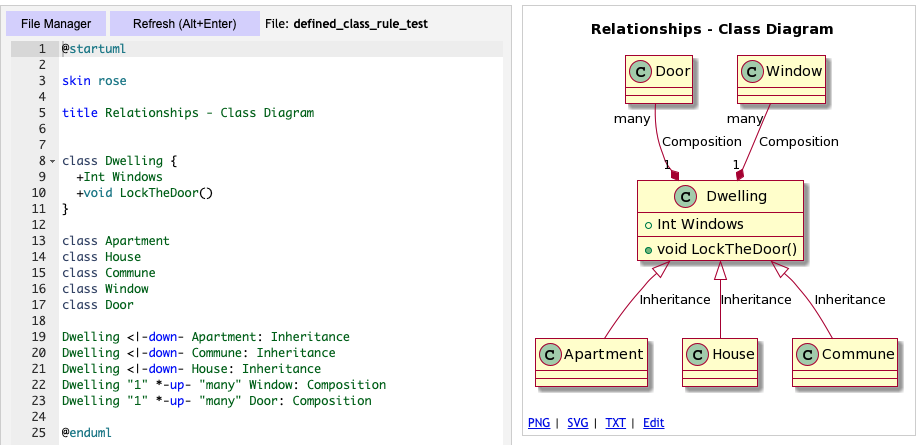
\includegraphics[width=15cm]{images/plantText}
    \caption{Grafische Benutzeroberfläche von plantText}
    \label{fig:plant-text}
\end{figure}

Vor der Wahl von PlantText als Instrument für die Entwurfsphase der Anwendung wurden mehrere Modellierungswerkzeuge
einer eingehenden Prüfung unterzogen. Diese Werkzeuge schlossen namhafte Anwendungen wie Enterprise Architect~\cite{enterarch},
Astah UML ~\cite{astah}, MagicDraw ~\cite{magic}, Visual Paradigm ~\cite{visual}, Umbrello ~\cite{umbrello} und Draw.io~\cite{draw} ein.
Eine gemeinsame Eigenschaft dieser Werkzeuge besteht darin, dass sie sich für die rasche Erstellung von Diagrammen
eignen, was auf ihre intuitive Benutzeroberfläche, leichte Verständlichkeit und Nutzerfreundlichkeit zurückzuführen ist.
Bedauerlicherweise wiesen sie jedoch einen bedeutenden Mangel auf, der ihre Anwendbarkeit in Bezug auf unsere
spezifischen Anforderungen einschränkte. Keines dieser Programme bot die Möglichkeit, die erstellten Diagramme in eine
leicht interpretierbare textuelle Form zu überführen.

Die meisten dieser Tools gestatten zwar das Exportieren der erstellten Diagramme im XML-Format, doch dieses Format
präsentiert lediglich eine räumliche Repräsentation der verschiedenen Objekte in einer Ebene, ohne eine semantische
Tiefenstruktur. Ein weiteres Hindernis bestand darin, dass die Informationen bezüglich der Verbindungen zwischen den
diversen UML-Objekten nur mit großem Aufwand und erheblichen Schwierigkeiten aus dem generierten XML extrahiert werden
konnten. Dies wäre in der Praxis äußerst zeitaufwendig und würde die Entwicklung eines eigenen Parsers erfordern, um die
relevanten Informationen zu extrahieren und in eine verwertbare Form zu überführen.

Die Nutzung von PlantText hingegen bietet einen klaren Vorteil in dieser Hinsicht. Dies resultiert aus der bereits
implementierten PlantUML-Engine, die über einen eingebauten Parser verfügt. Diese Funktionalität ermöglicht es,
den erstellten Code direkt in einem Format zu erhalten, das für die Weiterverarbeitung und Interpretation äußerst zugänglich ist.
Diese grundlegende Unterscheidung führt dazu, dass PlantText in unserem Anwendungsfall als überlegen angesehen wird.
Durch die Fähigkeit zur Bereitstellung des Modells in einer textuellen Form ermöglicht es eine tiefere und
bedeutungsvollere Analyse der erstellten Diagramme. Dies fördert die Genauigkeit bei der Modellierung und stellt sicher,
dass die erstellten Diagramme nicht nur als visuelle Darstellungen betrachtet werden, sondern auch als Quellen
semantischer Informationen dienen können.

\subsection{PlantUML Parser + Nodejs}

Im vorangegangenen Unterabschnitt wurde die Anwendung PlantText als Instrument zur Erstellung von Diagrammen
vorgestellt. Es ist jedoch essenziell zu betonen, dass PlantText lediglich die grafische Benutzeroberfläche darstellt,
da die zugrundeliegende Engine, auf der PlantText basiert, ``Plant-UML''~\cite{plantUML} ist. PlantUML ist ein Open-Source-Tool,
das von Arnaud Roques entwickelt wurde und erstmals im Jahr 2009 veröffentlicht wurde~\cite{plantUML}. Als Java-Anwendung
ermöglicht PlantUML, ähnlich wie PlantText, die Modellierung von Diagrammen, wobei die Verwendung durch die Entwicklung
von PlantText vereinfacht wurde. Alle im vorherigen Abschnitt hervorgehobenen Vorteile der Nutzung von PlantText sind in
Wirklichkeit Funktionen von PlantUML.

Eine besonders bemerkenswerte Funktion, die in diesem Abschnitt präsentiert und im Folgenden verwendet wird, ist jedoch
der PlantUML-Parser~\cite{plantUMLParser}. PlantUML ist im Wesentlichen eine Backend-Anwendung, die auf einem Server
ausgeführt wird. Wenn ein Benutzer ein Modell erstellen und Code in PlantText eingeben möchte, wird dieser Code an einen Server
übertragen, der ihn analysiert, interpretiert und ein Diagramm mithilfe von Graphviz~\cite{graphViz} generiert. Mit
Hilfe des PlantUML-Parsers besteht die Möglichkeit, das erzeugte Diagramm in ein Format zu exportieren, das für
programmatische Anwendungen geeignet ist. Es ist genau diese Funktion, die im weiteren Verlauf dieser Abhandlung
ausführlich behandelt wird.

Der PlantUML Parser~\cite{plantUMLParser} ist ein Open-Source-Tool,
mit dem der PlantUML-Code in ein JSON-Format geparst werden kann. Dieses Format kann zur Modellierung verschiedener
Regelobjekte (wie im Konzept beschrieben~\ref{sec:konzept}) verwendet werden. Da der Parser ausschließlich in einer
Serverumgebung funktioniert und somit in verschiedenen Java-, Node.js- und Python-Umgebungen verfügbar ist, kann er
ausschließlich in solchen Umgebungen eingesetzt werden.

Node.js~\cite{Node} wird verwendet, um diese Serverumgebung zu erstellen und eine gewisse Kohärenz zwischen dem
Frontend und dem Backend sicherzustellen, indem die Verwendung mehrerer Programmiersprachen in einem Projekt vermieden
wird. Dies trägt zur Effizienz und Integration des Gesamtprojekts bei.

\subsection{Vue.js}

Vue.js, oft auch einfach als Vue bezeichnet, ist  ein leistungsfähiges Open-Source-JavaScript-Framework, konzipiert und
entwickelt von Evan You~\cite{vue}. Der Ursprung von Vue.js entsprang der Vision, eine zeitgemäße, wandelbare und leicht
handhabbare Lösung zur Gestaltung von Benutzeroberflächen in Webanwendungen zu schaffen. In seiner Erstveröffentlichung
im Jahr 2014 initiiert, hat Vue.js eine bemerkenswerte Entfaltung erfahren, die es zu einem herausragenden Akteur unter
den JavaScript-Frameworks in der Sphäre der Webentwicklung gemacht hat.

In den Zielen und Vorzügen von Vue.js kristallisiert sich eine Antwort auf die Herausforderungen bei der Generierung
interaktiver Webanwendungen und die Optimierung des Entwicklungsprozesses in ein ergötzliches Narrativ. Wesentliche
Prämissen und Gewinnpunkte von Vue.js offenbaren sich in folgender Weise:

\begin{enumerate}
    \item \textbf{Nahtlose Integration:} Vue.js kann ohne Mühe in laufende Projekte integriert werden, unabhängig davon,
ob es als das Hauptframework oder als eine ergänzende Komponente in Kombination mit anderen Technologien fungiert.
Hierdurch ergibt sich ein gestaffelter Übergangsprozess und eine vorherrschende Flexibilität in der Architektur von
Anwendungen.
    \item \textbf{Komponentenbasierte Architektur:} Vue begünstigt die Einsetzung wiederverwendbarer Komponenten, die
nicht nur die Strukturierung und Organisation des Quellcodes erleichtern, sondern auch eine präzise Abgrenzung von
Aufgaben und eine verbesserte Wartbarkeit ermöglichen.
    \item \textbf{Reaktive Datenbindung:} Vue bietet eine reaktive Datenbindung, die die automatische Synchronisierung
von Daten und Benutzeroberfläche gestattet. Hierbei erfolgt die Anpassung von Daten an die Benutzeroberfläche und
umgekehrt ohne das Hinzufügen von Zusatzcode.
    \item \textbf{Deklarative Rendering:} Die Einbindung deklarativer Syntax in Vue.js vereinfacht die Implementierung
von Benutzeroberflächenelementen erheblich. Entwickler können die gewünschte Darstellung der Benutzeroberfläche
beschreiben, während Vue für die entsprechende Logikumsetzung sorgt.
    \item \textbf{Gemeinschaftsunterstützung:} Vue.js profitiert von einer florierenden und stetig wachsenden
Entwicklergemeinschaft, die eine Vielzahl von Ressourcen, Bibliotheken und Erweiterungen zur Verfügung stellt. Dies
vergrößert die Möglichkeiten zur Erweiterung und Anpassung von Vue-Projekten erheblich.
\end{enumerate}

Die Entscheidung zur Verwendung von Vue.js in einem Projekt kann vielschichtige Vorteile entfalten. Primär ermöglicht
die komponentenbasierte Architektur eine effiziente Code-Entwicklung, indem wiederverwendbare Komponenten zur
Strukturierung komplexer Benutzeroberflächen genutzt werden. Dies resultiert in einer verbesserten Wartbarkeit des
Quellcodes und einer beschleunigten Entwicklungszeit~\cite{wohlgethan2018supportingweb}.

Die reaktive Datenbindung von Vue.js bewirkt eine harmonische Synchronisation von Daten und Benutzeroberfläche, was die
Schöpfung interaktiver und ansprechender Webanwendungen begünstigt. Die deklarative Syntax von Vue reduziert
gleichzeitig den Boilerplate-Code und erleichtert die Nachvollziehbarkeit des Quellcodes. Vue.js ist zudem für seine
aktive Entwicklergemeinschaft und die Verfügbarkeit einer Vielzahl von Erweiterungen und
Plugins bekannt. Dies erlaubt den Zugriff auf bewährte Lösungen und bewährte Praktiken, was die Effizienz und Qualität
eines Projekts immens steigern kann~\cite{wohlgethan2018supportingweb}.

Schließlich bietet Vue.js eine attraktive Option für jene, die ein flexibles und gut dokumentiertes Framework suchen,
das sich reibungslos in bestehende Projekte einfügt. Vue kann schrittweise übernommen und je nach Projektanforderungen
sowohl als Hauptframework als auch für spezifische Aufgaben verwendet werden ~\cite{wohlgethan2018supportingweb}.

Zusammengefasst gewährleistet Vue.js eine stabile Grundlage für die Gestaltung zeitgemäßer, interaktiver Webanwendungen
und trägt entscheidend dazu bei, die Effizienz und Qualität von Projekten zu erhöhen. Vor diesem Hintergrund erweist
sich die Verwendung von Vue.js in diesem Projekt als empfohlen, um die Vorzüge dieses robusten Frameworks voll
auszuschöpfen. Für die Umsetzung des Konzepts wurden verschiedene andere Werkzeuge und Bibliotheken verwendet, jedoch
wurden in diesem Abschnitt nur die wichtigsten vorgestellt.

\section{Darlegung des Workflow-Prozesses}

\section{Einrichtung und Entwicklung des ``GReQL Converter''}
	\chapter{Evaluation}

Dieses Kapitel widmet sich einer umfassenden Analyse der Relevanz und Effektivität des GReQL Converters als innovatives
Werkzeug. Spezifisch zielt diese Abschnitt darauf ab, die grundlegende Frage zu beantworten, ob dieses Instrument
tatsächlich im akademischen und pädagogischen Kontext nützlich ist. Um dieses Ziel zu erreichen, ist es von größter
Wichtigkeit, eine systematische Herangehensweise zu verfolgen, die die Anwendung verschiedener Bewertungsmethoden
beinhaltet, um die Vorzüge und Effektivität des GReQL Converters nachzuweisen. Dieses Kapitel behandelt ausführlich die
angewandten Ansätze zur Prüfung des GReQL Converters, die Datensammlungsmethoden und die durchgeführten Analysen zur
Messung seiner Nützlichkeit. Letztendlich geht es darum, empirisch festzustellen, ob dieses Werkzeug konkrete Vorteile
und einen signifikanten Mehrwert für Lehrende und Lernende bietet.

\section{Erreichte Ziele}\label{sec:erreichte-ziele}

Die Untersuchung der Effizienz und Funktionalität des GReQL Converters als Instrument zur Extraktion relevanter
GReQL-Regeln aus einer UML-Diagrammannotation, die mittels PlantText zur Evaluation von UML-Diagrammen erstellt wurde,
stellt eine essenzielle Fragestellung dar, welche eine systematische und tiefgehende Herangehensweise erfordert. In dem
Implementierungskapitel (siehe Kapitel~\ref{ch:implementierung}) wurden diverse Regeln vorgestellt, begleitet von einer detaillierten Erläuterung des
spezifischen Extraktionsprozesses für jede dieser Regeldefinitionen. Gleichwohl erwies sich eine umfassende Testphase
als unverzichtbar, um eine eingehende Evaluierung der Leistungsfähigkeit jeder einzelnen Regel zu ermöglichen.

Zur Durchführung dieser Evaluierungen wurden verschiedene Testverfahren appliziert, welche eine Vielzahl von Szenarien
und Variationen abdeckten, mit dem Ziel, die Effizienz der durch den GReQL Converter generierten Regeldefinitionen
im Detail zu beurteilen. Der Testprozess kann in vier diskrete Schritte unterteilt werden:

\begin{enumerate}[itemsep=3pt, parsep=3pt]
    \item Initiale Generierung eines Diagramms mithilfe von PlantText, wobei dieses Diagramm gezielt konzipiert wurde,
um die spezifischen Merkmale der zu evaluierenden Regel zu inkorporieren. Zum Beispiel wurde ein Diagramm erstellt,
welches eine Aggregation zwischen zwei Klassen darstellte, um eine Regel zur Aggregation zu prüfen.
    \item Erstellung eines Evaluationsdiagramms (welches in diesem Kontext mittels BOUML modellisiert wurde), welches von
den generierten Regeldefinitionen bewertet werden sollte.
    \item Extraktion der verschiedenen Regeldefinitionen aus dem PlantText-Code.
    \item Evaluierung mithilfe der GReQL-Engine von JACK, um festzustellen, ob die Regeldefinitionen die Aggregation
im Diagramm effektiv erkannt haben.
\end{enumerate}

Parallelen dazu wurde besonderes Augenmerk auf die Identifikation von falsch positiven (False Positiv) Ergebnissen
gerichtet, welche den Eindruck einer korrekten Funktionsweise des Werkzeugs erwecken könnten, obwohl dem nicht so ist.
Hierzu wurde eine sorgfältige Analyse des generierten Codes durchgeführt, und die Protokolle der GReQL-Engine wurden
überprüft, um die präzise Identifikation der Aggregationsregel sicherzustellen. Es sei hervorgehoben, dass dieser
gewissenhafte Überprüfungsprozess in systematischer Weise auf alle vorab definierten Regeldefinitionen der
Implementierungsphase angewandt wurde.

Im Anschluss an die individuelle Prüfung jeder Regeldefinition erfolgte eine Evaluierung anhand zunehmend komplexerer
Diagramme. Das Ziel bestand darin, mehrere Funktionen simultan zu bewerten und zu ermitteln, ob die Existenz mehrerer
Verknüpfungen zwischen verschiedenen Elementen im Diagramm spezifische Regeldefinitionen nicht beeinträchtigte. Die
Bedingungen, die zu potenziellen Konflikten führen könnten, wurden somit eingehend untersucht, und der GReQL Converter
wurde bei jeder Fehlererkennung oder -identifikation angepasst, um seine Effizienz zu steigern.

In einem darauffolgenden Schritt wurden verschiedene gängige Übungen zu UML-Diagrammen selektiert, um die akademische
Leistung der Studierenden an der Universität zu evaluieren. Unter diesen Übungen findet sich das Diagramm ``Mendelssohn
\& Sohn Maschinenbau GmbH'', welches im Rahmen des Kurses ``Einführung in die Unified Modeling Language'' an der
Universität Potsdam zum Einsatz kam (siehe Abbildung~\ref{fig:bau_gmbh}). Dieses spezifische Diagramm weist signifikante
Ähnlichkeiten zu den traditionellen Modellen auf, die in universitären Prüfungskontexten verwendet werden, wodurch es
sich als exemplarisches Testobjekt zur Ermittlung der Leistungsfähigkeit des GReQL Converters erweist.

Zu diesem Ziel wurde das Musterdiagramm, das als Repräsentation der Übungsvorlage diente, mittels des Werkzeugs
BOUML modelliert. Anschließend erfolgte die Extraktion der XMI-Datei, welche als Bewertungsinstrument diente. Parallel
dazu wurde die Anwendung von PlantText zur Erstellung der Musterdiagrammvorlage in Erwägung gezogen, wobei der GReQL
Converter im Anschluss dazu verwendet wurde, um die Regeln gemäß dem vorab beschriebenen Verfahren formal zu erfassen.
Subsequent zur Extraktion der Regeldefinitionen und der willkürlichen Punktevergabe für jede einzelne Regel, unterzog
man diese Regeldefinitionen einer Evaluation im Rahmen des GReQL-Motors von JACK.

Hervorzuheben ist, dass für ein mittelkomplexes Diagramm wie das genannte insgesamt \textbf{82 GReQL-Regeln} generiert
wurden. Nach abschließenden Tests ergab sich, dass der GReQL-Motor eine Erfolgsrate von 100\% aufwies, was auf die
korrekte Funktionalität der erzeugten Regeldefinitionen hinweist. Dieser Erfolg illustriert eindrucksvoll die Befähigung
des GReQL Converters zur effektiven Evaluierung von UML-Diagrammen, insbesondere jener von erhöhter Komplexität.

\begin{figure}[h]
    \centering
    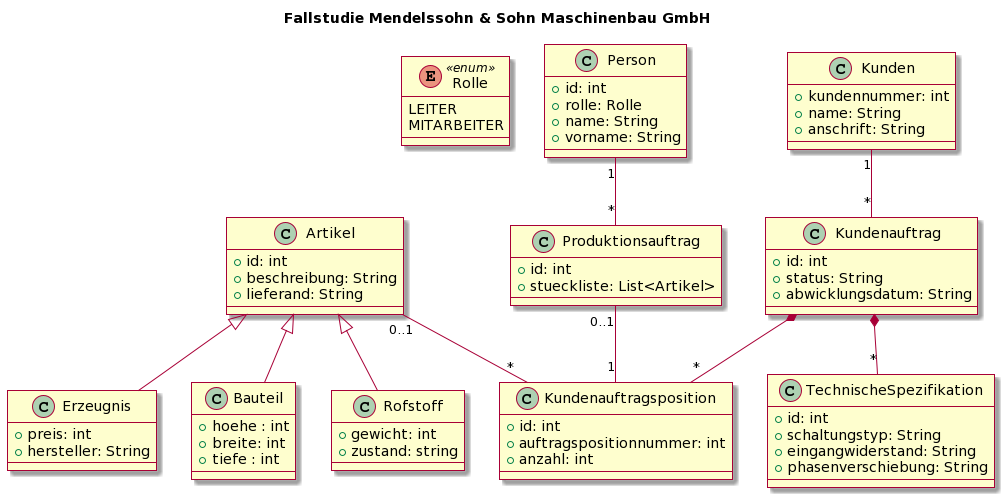
\includegraphics[width=16cm]{images/bau_gmbh_plantText}
    \caption{Fallstudie UML - Klassendiagramm}
    \label{fig:bau_gmbh}
\end{figure}

In Bezug auf die Leistungen, die dem GReQL Converter zugeschrieben werden können, lassen sich folgende Punkte
feststellen:

\begin{enumerate}[itemsep=3pt, parsep=5pt]
    \item Der GReQL Converter ermöglicht die umfassende Bewertung eines Diagramms. Im vorherigen Beispiel ermöglichte er
die Generierung von 82 Regeln, eine Aufgabe, die besonders mühsam und fehleranfällig wäre, wenn sie manuell von einem
Lehrer durchgeführt würde.
    \item Der GReQL Converter führt Bewertungen äußerst präzise durch und verhindert somit potenzielle Fehler, die
Lehrer bei manuellen Bewertungen begehen könnten.
    \item Der GReQL Converter verhindert Fehler in Bezug auf die Syntax und Formulierung von Regeln, insbesondere
solche, die bereits vom Tool definiert sind, was den Benutzer von Sorgen in Bezug auf diese Aspekte entlastet.
    \item Darüber hinaus ist eine direkte Interaktion mit dem GReQL-Code nicht mehr erforderlich, da der Benutzer die
Regeln problemlos ändern kann, indem er die generierten Objekte nach dem Schritt der syntaktischen Analyse verwendet,
was den Bearbeitungsprozess vereinfacht.
    \item Der GReQL Converter erleichtert erheblich das Verständnis des GReQL-Codes, indem er klaren, lesbaren und
zugänglichen Code generiert, was es Dritten ermöglicht, seine Funktionsweise zu verstehen und bei Bedarf Änderungen
vorzunehmen.
    \item Darüber hinaus berücksichtigt das Design des Tools die Vielfalt grundlegender Varianten in UML-Diagrammen,
was seine Vielseitigkeit und Anpassungsfähigkeit stärkt.
\end{enumerate}

Wenn man diese Vorteile mit den in Teil drei aufgeführten Problemen vergleicht, die die
Problemanalyse (siehe Kapitel~\ref{ch:problemanalyse}) behandelten, steht außer Frage, dass der GReQL Converter seine Rolle als
Hilfsmittel bei der Erstellung von GReQL-Code für die Bewertung von Klassendiagrammen erfüllt und Lehrern erheblich
Zeit spart. Im nächsten Abschnitt wird eine Studie durchgeführt, um zu ermitteln, ob Lehrende diese Ansicht teilen.

\section{Interview zur Bewertung des GReQL Converters}

Im vorherigen Kapitel wurde der GReQL Converter auf seine Funktionen hin getestet, um potenzielle Fehler zu erkennen und
zu beheben. Es war jedoch von entscheidender Bedeutung, externe Rückmeldungen und Kommentare einzuholen, um weitere
Verbesserungsansätze zu identifizieren, neue Ideen zu generieren und die Grenzen des Tools aufzuzeigen. Aus diesem Grund
wurde beschlossen, Interviews mit verschiedenen wissenschaftlichen Mitarbeitern durchzuführen, die bereits Erfahrung
mit GReQL-Code haben, um das Tool zu testen.

Das Interview erwies sich als das geeignetste Modell, da es bereits die Möglichkeit bietet, direkte Fragen zu stellen
und ein lebhafteres Feedback zu erhalten sowie detaillierte und umfassende Antworten vom Befragten zu erhalten. Darüber
hinaus ermöglicht das Interviewformat eine gewisse Flexibilität, da zukünftige Fragen je nach den erhaltenen Antworten
angepasst werden können. Dieses Format erleichtert auch die Kontextualisierung. Falls eine Frage nicht verstanden wird,
kann der Befragte Nachfragen stellen, um im Kontext zu bleiben. Im folgenden Abschnitt wird zunächst die
Interviewkonzeption sowie der Prozess und die Ergebnisse des Interviews diskutiert.

\subsection{Konzeption des Interviews}

Das Ziel des Interviews besteht darin, das Feedback verschiedener Lehrer zum GReQL Converter zu sammeln und die
Möglichkeiten zur Verbesserung des Tools zu erörtern. Am Ende des Interviews wird es möglich sein festzustellen, ob
das Tool einen echten Nutzen für die Benutzer hat und ob es sinnvoll ist, seine Entwicklung fortzusetzen. Um dies zu
erreichen, war es zunächst erforderlich, die verschiedenen Lehrer anhand bestimmter Kriterien zu qualifizieren,
darunter:

\begin{enumerate}[itemsep=3pt, parsep=5pt]
    \item Die Lehrer sollten bereits wissen, was GReQL ist.
    \item Die Lehrer sollten bereits GReQL-Code geschrieben haben, um ein UML Klassendiagramm zu bewerten.
\end{enumerate}

Das Interview erstreckt sich tatsächlich über fünf Phasen, von der Vorbereitung bis zum Fragebogen:

\subsubsection{PHASE 1: Vorbereitung auf das Interview}

Während des Interviews sollte der Schwerpunkt auf dem GReQL Converter liegen. Um zu verhindern, dass die Lehrer
während des Interviews mit dem Schreiben von PlantText-Code beschäftigt sind, wurde beschlossen, sicherzustellen,
dass die Lehrer vor dem Interview den PlantText-Code schreiben, den sie während des Interviews benötigen werden. Zu
diesem Zweck sollen die interviewten Personen eine Übung durchführen, die sie mit dem PlantText-Tool und plantUML
vertraut macht.

Bei der Einladung zum Interview wurde ein Bild ausgewählt und an die Lehrer gesendet, das bereits sein äquivalentes XMI
generiert hat, das später verwendet wird, um den generierten GReQL-Code auf JACK zu testen. Da das Hauptziel darin
besteht, GReQL-Code aus PlantText zu generieren, sollen die Lehrer versuchen, die Musterlösung auf PlantText zu
reproduzieren:

\begin{enumerate}[itemsep=5pt, parsep=5pt]
    \item Wenn sie dies schaffen, müssen sie ihren PlantText-Code lediglich mit dem GReQL Converter annotieren, die
Lösung auf JACK testen und die während des Interviews gestellten Fragen beantworten.
    \item Wenn sie dies nicht geschafft haben, wird ihnen der PlantText-Code zur Verfügung gestellt und erklärt, wie
dieser Code erstellt wurde, einschließlich einiger Feinheiten. Anschließend sollen sie diesen PlantText-Code mit dem
GReQL Converter annotieren und die während des Interviews gestellten Fragen beantworten.
\end{enumerate}

Es ist auch wichtig, den Lehrern die Dokumentation zum GReQL Converter sowie den Zugang zum Tool zur Verfügung zu
stellen, damit sie es vor dem Interview testen und sich damit vertraut machen können, wenn ihre Verfügbarkeit dies
zulässt.

\subsubsection{PHASE 2: Einführung in das Interview}

In dieser Phase geht es darum, den GReQL Converter vorzustellen, seine Feinheiten, Funktionen sowie seine Verwendung und
Dokumentation zu präsentieren. Das Ziel dieser Phase besteht darin, die Lehrer mit dem Tool vertraut zu machen und
ihnen alle notwendigen Informationen für den weiteren Verlauf zur Verfügung zu stellen.

\subsubsection{PHASE 3: Annotation des PlantText-Codes}

In dieser Phase müssen sich die Lehrer auf die Annotation des PlantText-Codes im GReQL Converter konzentrieren. Sie
verwenden das Tool zur Generierung von GReQL-Code.

\subsubsection{PHASE 4: Test des generierten GReQL-Codes}

In dieser Phase müssen die Lehrer den generierten GReQL-Code auf JACK testen. Zu diesem Zweck wurden entsprechende
Übungen bereits auf der Plattform vorbereitet, um den Prozess zu erleichtern. Sie müssen lediglich ihren GReQL-Code
sowie das zuvor vorbereitete XMI eingeben, um ihn zu testen.

\subsubsection{PHASE 5: Fragebogen}

Am Ende des Interviews werden den Lehrern eine Reihe von vorbereiteten Fragen gestellt, um ihre Erfahrungen, Meinungen
und Verbesserungsvorschläge für den GReQL Converter zu bewerten. Die während des Interviews gestellten Fragen sind
wie folgt:

\begin{enumerate}[itemsep=5pt, parsep=5pt]
    \item \textbf{Einführung in das Tool:}
    \begin{enumerate}
        \item Können Sie kurz erklären, was das Tool GReQL Converter Ihrer Meinung nach ist?
        \item Haben Sie bereits ähnliche Tools zur Generierung von GReQL-Code aus UML-Diagrammen verwendet?
    \end{enumerate}
    \item \textbf{Benutzererfahrung:}
    \begin{enumerate}
        \item Wie empfanden Sie die Benutzeroberfläche des GReQL Converters in Bezug auf Benutzerfreundlichkeit?
        \item Können Sie die Schritte beschreiben, die Sie unternommen haben, um das Tool zu verwenden, von der
        Code-Importierung aus PlantText bis zur Generierung von GReQL-Code?
        \item Ist das Tool intuitiv?
        \item Konnten Sie auf einen Blick verstehen, was Sie tun mussten?
        \item Gab es Probleme oder Hindernisse bei der Verwendung des Tools?
    \end{enumerate}
    \item \textbf{Dokumentation:}
    \begin{enumerate}
        \item Haben Sie die Dokumentation des GReQL Converters konsultiert?
        \item Wenn ja, wie fanden Sie sie in Bezug auf Klarheit und Nützlichkeit?
        \item Gibt es Aspekte des Tools oder seiner Funktionsweise, die Sie in der Dokumentation nicht
        verstanden haben und die Sie gerne darin gefunden hätten?
    \end{enumerate}
    \item \textbf{Generierung von GReQL-Regeln:}
    \begin{enumerate}
        \item Wie würden Sie die Genauigkeit des Tools bei der Generierung von GReQL-Regeln aus mit PlantText
        erstellten UML-Diagrammen bewerten?
        \item Gab es Fehler oder Inkonsistenzen in den generierten Regeln?
    \end{enumerate}
    \item \textbf{Vergleich des Tools mit der manuellen Methode:}
    \begin{enumerate}
        \item Wie würden Sie die Effizienz des GReQL Converters im Vergleich zur manuellen Erstellung von GReQL-Regeln
        aus UML-Diagrammen in Bezug auf Zeitersparnis und Genauigkeit bewerten?
        \item Können Sie konkrete Beispiele nennen, in denen das Tool besonders nützlich oder weniger effektiv als
        die manuelle Methode war?
    \end{enumerate}
    \item \textbf{Verbesserungsvorschläge:}
    \begin{enumerate}
        \item Haben Sie Vorschläge zur Verbesserung der Benutzeroberfläche oder der Funktionen des GReQL Converters?
        \item Gibt es zusätzliche Funktionen, die Sie gerne im Tool sehen würden?
    \end{enumerate}
    \item \textbf{Nützlichkeit und Relevanz:}
    \begin{enumerate}
        \item Halten Sie das Tool GReQL Converter im Kontext der Bewertung von UML-Diagrammen für nützlich?
        \item Warum oder warum nicht?
    \end{enumerate}
    \item \textbf{Gesamtbewertung:}
    \begin{enumerate}
        \item Auf einer Skala von 1 bis 5, wobei 1 ``nutzlos'' und 5 ``äußerst nützlich'' bedeutet, wie würden Sie die
        Nützlichkeit des GReQL Converters bewerten?
        \item Auf einer Skala von 1 bis 5, wobei 1 ``sehr schlecht'' und 5 ``ausgezeichnet'' bedeutet, wie würden Sie
        das Design des GReQL Converters bewerten?
        \item Auf einer Skala von 1 bis 5, wobei 1 ``sehr schlecht'' und 5 ``ausgezeichnet'' bedeutet, wie würden Sie
        die Benutzerfreundlichkeit des GReQL Converters bewerten?
        \item Würden Sie dieses Tool anderen Fachleuten empfehlen, die mit UML-Diagrammen zur Bewertung arbeiten?
    \end{enumerate}
    \item \textbf{Allgemeines Feedback:}
    \begin{enumerate}
        \item Haben Sie weitere Kommentare, Vorschläge oder Beobachtungen, die Sie zum GReQL Converter teilen möchten?
    \end{enumerate}
\end{enumerate}

Die grundlegende Struktur der Interviews und die Wahl der Fragen wurden maßgeblich von den Erkenntnissen und Ratschlägen
des Autors Ian Brace in seinem Werk ``Questionnaire Design: How to Plan, Structure and Write Survey Material for
Effective Market Research'' beeinflusst~\cite{brace2018questionnaire}. Dieses Buch bietet umfassende Einblicke in
bewährte Methoden zur Gestaltung von Fragen und zur Strukturierung von Umfragen, die sich auch auf die
Interviewkonzeption übertragen lassen. Bei der Gestaltung der Fragen zur Benutzererfahrung und Benutzerfreundlichkeit
wurde das Buch ``Designing and Conducting Survey Research: A Comprehensive Guide'' von Louis M. Rea und Richard
A. Parker~\cite{rea2014designing} herangezogen, um die Best Practices für die Benutzerfreundlichkeit von Fragen zu
verstehen. Online-Umfrageplattformen wie SurveyMonkey~\cite{monkey} dienten als Inspiration für die Erstellung des
Interviewleitfadens und halfen bei der Identifizierung bewährter Praktiken zur Erstellung von Fragen und zur
Strukturierung von Umfragen. Im kommenden Abschnitt steht die Präsentation einer Auswahl der Ergebnisse nach den
Interviews im Vordergrund.


\subsection{Ergebnisse des Interviewverfahrens}

Die Interviews wurden mit einer Gruppe von fünf wissenschaftlichen Mitarbeitern von zwei Hochschulen geführt, nämlich
der Universität Duisburg-Essen und der Technischen Hochschule Köln (siehe Tabelle~\ref{tab:personnen}).

\begin{table}
    \centering
    \caption{Befragte wissenschaftliche Mitarbeiter} \label{tab:personnen}
    \begin{adjustbox}{scale=0.9}
        \begin{tabular}{ll}
            \toprule
            \textbf{Hochschule} & \textbf{Lehrkraft} \\
            \midrule
            Universität Duisburg Essen & Dr. Michael Striewe \\
            \midrule
            Universität Duisburg Essen & Tobias Stottrop \\
            \midrule
            Universität Duisburg Essen & Christoph Olbricht \\
            \midrule
            Technische Hochschule Köln & Paul Hufnagel \\
            \midrule
            Technische Hochschule Köln & Prof. Dr. Mario Winter \\
            \bottomrule
        \end{tabular}
    \end{adjustbox}
\end{table}

\subsubsection{Interview mit Christoph Olbricht}
Christoph Olbricht, wissenschaftlicher Mitarbeiter an der Universität Duisburg-Essen, hat bereits GReQL-Code für die
Auswertung von Java-Übungen geschrieben. Allerdings fehlt ihm Erfahrung in der Auswertung von UML-Diagrammen. Das
Interview begann mit einer Vorstellung des GReQL Converters, einschließlich seiner Funktionen und Dokumentation. Vor
dem Interview erhielt Herr Olbricht per E-Mail ein UML-Diagramm, für das er im Voraus PlantText-Code schrieb. Während
des Interviews übertrug er den Code auf den GReQL Converter, annotierte ihn und führte mehrere Modifikationen durch.
Nachfolgend generierte er GReQL-Code, der erfolgreich auf JACK getestet wurde, wobei eine Bewertung von 100\% erreicht
wurde. Am Ende des Interviews wurden Fragen aus dem vorherigen Abschnittsfragebogen gestellt, um ein spezifisches
Feedback zum Tool zu erhalten.

\begin{enumerate}[itemsep=8pt, parsep=5pt]
    \item \textbf{Einführung in das Tool:}

    Gemäß seinen exakten Worten zum GReQL Converter: ``Mit diesem Tool können wir auf einfache und intuitive Weise
    GReQL-Code aus PlantText generieren und ihn auf sehr angenehme Art und Weise anpassen.'' Er hatte zuvor kein
    ähnliches Tool für die Generierung von GReQL-Code für Klassendiagramme verwendet.

    \item \textbf{Benutzererfahrung:}

    Entsprechend seiner exakten Worte zur Benutzerfreundlichkeit der Anwendung: ``Unheimlich angenehm. Vorher hatten wir
    ein ähnliches Tool für Java, aber dabei musste man seinen Java-Code einlesen und dann einen GReQL-Code einwerfen,
    um zu sehen, ob es funktioniert. Es war nur zum Testen gedacht. Bei deinem Tool ist es jedoch besonders angenehm,
    dass man die komplette Regel direkt erhält und sie nach Bedarf anpassen kann. Dadurch muss ich GReQL eigentlich
    nicht beherrschen, was für unsere Kunden unheimlich nützlich wäre.''

    Herr Olbricht fand das Tool intuitiv und war überrascht, dass die Regeln direkt generiert wurden, ohne dass eine
    umfangreiche Vorarbeit mit Annotationen geleistet werden musste. Das Tool macht viel mehr, als er erwartet hatte.
    Er hätte gerne einen Text gehabt, der den Prozess der Regelgenerierung sowie die Grundregeln klar erklaert und er
    betont am Ende: ``Aber intuitiv genug war das definitiv''.

    \item \textbf{Dokumentation:}

    Er lobte die Dokumentation als ausgezeichnet, ausgewogen und präzise. Die Menge an Inhalten wurde als angemessen empfunden.
    
    \item \textbf{Generierung von GReQL-Regeln:}

    Soweit er sehen konnte, waren die erstellten Regeln sehr genau und frei von potenziellen Fehlern. Er erwähnte auch,
    dass es ziemlich schwierig sei, Fehler mit einem einzigen Test zu identifizieren, aber dafür müsste man mehrere 
    Varianten des XMI-Dokuments der Musterlösung haben.
    
    \item \textbf{Vergleich des Tools mit der manuellen Methode:}

    Entsprechend seiner exakten Worte: ``Das ist eine wahnsinnige Zeitersparnis. Wenn ich diesen GReQL-Code selbst
    geschrieben hätte, hätte ich ihn 5, 6, 7 Mal testen müssen, um zu überprüfen, ob ich keine Fehler gemacht hätte,
    und ich hätte mich bestimmt irgendwann mal vertippt. Ich hätte vermutlich ungefähr 2-3 Stunden gebraucht, um alle
    Regeln zu schreiben. Aber mit dem Tool kann man einfach die Musterlösung importieren und los geht's.''

    \item \textbf{Verbesserungsvorschläge:}

    Herr Olbricht schlug vor, dass es nützlich wäre, unabhängiges Scrollen im PlantText-Code und den generierten
    GReQL-Regeln zu ermöglichen, um einen direkten Vergleich zu erleichtern. Er erwähnte auch, dass man auf dem
    Bildschirm einen Fehler anzeigen kann, wenn man sich bei einer Annotation in der Syntax vertan hat
    (z. B. wenn man vor der Annotation bestimmter Regeln die ``:'' vergisst).

    \item \textbf{Nützlichkeit und Relevanz:}

    Er fand das Tool sehr nützlich, da es vor allem eine enorme Zeitersparnis mit sich bringt.
    
    \item \textbf{Gesamtbewertung:}

    Er bewertete den GReQL Converter insgesamt mit \textbf{5 von 5 Punkten} in den Kategorien \textbf{Nützlichkeit},
    \textbf{Design} und \textbf{Benutzerfreundlichkeit}. Das Tool wurde als äußerst hilfreich und empfehlenswert für 
    Fachleute eingestuft. Er sagte, wenn das Tool in Produktion sei, könne er es tatsächlich anderen Fachleuten
    empfehlen. Nach seinen Worten: ``Nicht krakeln zu müssen, um welche Regel erzeugt werden soll, ist einfach nur
    nützlich.''

    \item \textbf{Allgemeines Feedback:}

    Herr Olbricht äußerte kein weiteres Feedback und bezeichnete das Tool als ``super''.
\end{enumerate}

\subsubsection{Interview mit Dr. Michael Striewe}

Dr. Michael Striewe ist ein wissenschaftlicher Mitarbeiter an der Universität Duisburg-Essen. Er ist eines der
Teammitglieder, das die Plattform JACK pflegt und weiterentwickelt. Zusätzlich dazu verfügt er über umfangreiche
Erfahrung mit GReQL, da er die Idee einbrachte und umsetzte, GReQL-Code zur Auswertung von Klassendiagrammen zu
nutzen~\cite{striewe2011automated}. Daher verfügt er über Fachwissen im Schreiben von GReQL-Code und in der Auswertung
von Diagrammen. Wie bei Christoph Olbricht begann das Interview mit einer Vorstellung des GReQL Converters sowie seiner
Dokumentation. Anschließend sollte Dr. Michael Striewe dieselbe Aufgabe wie herr Olbricht durchführen: Code in PlantText
für ein Klassendiagramm generieren. Danach annotierte er das Diagramm und testete es auf der Plattform JACK, wo er
zunächst ein Ergebnis von 96\% erzielte, aufgrund von zwei Fehlern. Insbesondere wurde die Syntax zum Schreiben eines
Enums gemäß der Dokumentation nicht eingehalten und es gab einen Tippfehler bei der Eingabe eines Klassennamens in der
XMI-Musterlösung. Genauer gesagt handelte es sich um den Namen einer Klasse ``Rofstoff'', der in der Standardlösung
falsch geschrieben war. Der korrekte Name sollte ``Rohstoff'' sein. Da er den Fehler bei der Erstellung der Regeln behob
und einen exakten Abgleich für den Klassennamen verwendete, erkannte JACK den Fehler. Dieses Verhalten ist keine
Programmierfehler oder ein Problem mit dem Tool, sondern vielmehr ein Beweis dafür, dass das Tool zuverlässig arbeitet
und wie erwartet funktioniert. Am Ende des Interviews wurden Fragen aus dem vorherigen Abschnittsfragebogen gestellt,
um ein spezifisches Feedback zum Tool zu erhalten.

\begin{enumerate}[itemsep=8pt, parsep=5pt]
    \item \textbf{Einführung in das Tool:}

    Dr. Michael Striewe hat das Wesen des GReQL Converters erfasst. Er beschrieb ihn als ein Werkzeug, das es
    ermöglicht, aus dem PlantUML-Code eines Klassendiagramms GReQL-Code zu generieren. Er hatte zuvor keine Erfahrung
    mit einem solchen Tool in Bezug auf die Auswertung von UML-Diagrammen mittels
    GReQL.

    \item \textbf{Benutzererfahrung:}

    Bezüglich Benutzererfahrung äußerte er: ``Es war relativ einfach zu bedienen. Allerdings muss man viel hin und her
    scrollen. Ansonsten ist es relativ intuitiv und ich bin ziemlich gut damit klargekommen.'' Jedoch hatte er zu Beginn
    einige Probleme bei der Verwendung des GReQL Converters. Als er seinen PlantText-Code auf die Plattform kopierte,
    konnten nur Klassendefinitionen (``Class Definition'') Regeln generiert werden, während die Assoziationsregeln nicht
    erkannt wurden. Dies lag daran, dass die Klassennamen in den Assoziationen in Anführungszeichen standen, was der
    Parser nicht erkennen konnte. Um dieses Problem zu beheben, musste der Benutzer sich an die in der Tool-Dokumentation
    definierte Syntax halten, und auf Entwicklerseite war es wichtig, den Benutzer zu benachrichtigen, wenn solche Fälle
    auftreten, damit er das Problem ohne weitere Untersuchungen verstehen kann.

    \item \textbf{Dokumentation:}

    Die Dokumentation fand er leicht verständlich und nützlich. Er wünschte sich jedoch, dass bestimmte Funktionen,
    wie die Definition des Enums, stärker hervorgehoben würden.

    \item \textbf{Generierung von GReQL-Regeln:}

    Hinsichtlich der Präzision des Tools glaubt Dr. Michael Striewe, dass ein einzelnes Beispiel nicht ausreicht, um
    diesen Aspekt zu testen. Es wäre notwendig, es mit mehreren Lösungen und unterschiedlichen Diagrammen mit mehr oder
    weniger Fehlern zu testen, um zu sehen, ob die vom GReQL Converter generierten Regeln die Feinheiten erkennen. Er
    erwähnte auch die Möglichkeit, dass verschiedene Diagramme, die auf PlantText identisch sind, unterschiedliche
    Regeln generieren könnten, je nach verwendeter Syntax. Seiner Meinung nach sollte das Tool in verschiedenen
    Varianten getestet werden. Ein einzelnes Beispiel reicht nicht aus, um diese Frage zu beantworten.


    Hinsichtlich der Unstimmigkeiten im generierten GReQL-Code hatte er bis zum Zeitpunkt des Interviews nichts
    Auffälliges bemerkt. Er betonte jedoch auch, dass er die Regeln nicht einzeln überprüft hatte, was ebenfalls
    weitere Untersuchungen erfordert.


    \item \textbf{Vergleich des Tools mit der manuellen Methode:}

    Dr. Michael Striewe ist der Ansicht, dass durch die Verwendung des GReQL Converters viel Zeit gespart werden kann.
    Um das zu annotierende PlantText-Diagramm zu generieren, benötigte er nur 15 Minuten und konnte von dort aus mehr
    als zwanzig Regeln erstellen. Das empfand er als äußerst schnell und er könnte sich nicht vorstellen, die gleiche
    Aufgabe manuell genauso schnell zu erledigen. Er findet das Tool sehr effektiv bei Regeln, die viel Copy-and-Paste
    erfordern (zum Beispiel bei Attributregeln, Klassendefinitionen und Methoden).

    Dort, wo das Tool weniger effektiv sein könnte, wären spezielle Varianten, insbesondere Fälle, in denen spezifische
    Varianten von Klassennamen gefordert sind. Zum Beispiel, wenn Regeln erstellt werden müssen, bei denen die
    Klassennamen genau ``Kunde'' oder ``Kunden'' sein müssen, wäre es einfacher, dies manuell zu tun als den GReQL
    Converter zu nutzen.

    \item \textbf{Verbesserungsvorschläge:}

    \begin{itemize}[itemsep=8pt, parsep=5pt]
        \item Die Bezeichnung des ``Delete''-Buttons sollte in ``Disable'' geändert werden, um nicht mehr für die
        Generierung des GReQL-Codes in Betracht gezogen zu werden. Dadurch könnte die Möglichkeit geschaffen werden,
        bestimmte Codevarianten zu testen. Mit ``Delete'' wird die Regel gelöscht und der Code muss erneut geparst
        werden, alle zuvor vorgenommenen Änderungen gehen verloren. ``Disable'' könnte mehr Flexibilität bei der
        Generierung der Regeln bieten.
        \item Der GReQL Converter sollte in der Lage sein, verschiedene Modellierungsvarianten von Regeln zu
        ermöglichen. Nicht nur Varianten in Bezug auf die Klassennamen, sondern auch die Möglichkeit, mehrere
        Modellierungsvarianten einer Regel zu haben. Derzeit generiert der GReQL Converter nur Regeln für einen
        einzigen Diagrammtyp. Es ist jedoch möglich, dass Studenten verschiedene Diagrammtypen erstellen, die alle
        korrekt sind. Im Fall von ``Sohn Maschinenbau GmbH'' (siehe Abschnitt~\ref{sec:erreichte-ziele}) könnte es möglich sein,
        ``stueckliste'' entweder als Attribut oder als Assoziation zu modellieren. Es gibt auch Fälle, in denen Student
        eine einfache Assoziation anstelle einer Aggregation verwenden könnten, und die Modellierung wäre immer noch
        korrekt. Der GReQL Converter sollte diese Funktionalität hinzufügen können.
        \item Der GReQL Converter sollte auch die Möglichkeit bieten, GReQL-Code nur für eine einzelne Regel zu
        generieren. Das könnte die Änderung von Regeln erheblich erleichtern.
    \end{itemize}

    \item \textbf{Nützlichkeit und Relevanz:}

    In Bezug auf die Nützlichkeit und Relevanz des Tools sagte Dr. Michael Striewe: ``Ja, definitiv, es ist nützlich.
    Es erleichtert mir zunächst einmal das schnelle Erstellen einer großen Anzahl von Regeln. Danach muss ich jedoch
    vieles manuell nacharbeiten. Aber der Aufwand, zunächst einmal die Regeln zu erstellen, ist bereits erledigt.''


    \item \textbf{Gesamtbewertung:}

    Er bewertete den GReQL Converter insgesamt mit \textbf{5 von 5 Punkten} in den Kategorien \textbf{Design} und
    \textbf{Benutzerfreundlichkeit}, sowie mit \textbf{4 von 5 Punkten} für die \textbf{Nützlichkeit}, da er noch
    Erwartungen und Wünsche für Verbesserungen hat. Das Tool wurde als äußerst hilfreich und empfehlenswert
    für Fachleute eingestuft.

\end{enumerate}

\subsubsection{Interview mit Tobias Stottrop}

Tobias Stottrop, wissenschaftlicher Mitarbeiter an der Universität Duisburg-Essen, hat bereits GReQL-Code für die
Auswertung von UML Klassendiagrammen im Rahmen des Vorlesung ``Software Systeme'' verwendet. Tobias hatte das Interview
nicht vorbereitet, da er sich nicht auf der JACK-Plattform registriert hatte und auch nicht den erforderlichen
PlantText-Code für die Diagrammbewertung geschrieben hatte. Daher wurde während des Interviews ein anderer Ansatz
verfolgt. Basierend auf seiner Erfahrung mit GReQL und einer kurzen Einführung und Demonstration von PlantText ging
es darum, verschiedene Anwendungsfälle des GReQL Converters zu testen, um zu analysieren, was möglich ist und welche
Punkte noch verbessert werden müssen. Das Interviewmodell war anders als zuvor durchgeführte.

\begin{enumerate}[itemsep=8pt, parsep=5pt]
    \item \textbf{Einführung in das Tool:}

    Tobias Stottrop hat verstanden, was der GReQL Converter ist. In seinen eigenen Worten erklärte er:
    ``Es handelt sich um ein Hilfswerkzeug zur Generierung von GReQL-Code für UML-Diagramme. Es basiert auf einer
    Beschreibungssprache namens PlantUML und dient der Generierung von XMI-Code.'' Er hatte zuvor kein solches Tool
    verwendet und glaubt, dass der GReQL Converter das erste seiner Art ist.

    \item \textbf{Benutzererfahrung:}

    Er fand die Syntax-Hervorhebung sehr angenehm und meinte, dass dies die Benutzererfahrung mit dem GReQL Converter
    verbessert. Er erwähnte auch, dass es schwierig sein kann, bei einem sehr umfangreichen Diagramm den Überblick
    zu behalten, mit Code auf der einen Seite und mehreren generierten Regeln auf der anderen Seite. Er betonte jedoch,
    dass er darüber nicht urteilen könne, da ihm kein solches Beispiel vorliegt.

    Er empfand das Tool insgesamt als sehr intuitiv. Aber er erwähnte, dass bestimmte Funktionen, wie das Hinzufügen von
    manuellen Regeln, nicht auf Anhieb zu finden waren. Außerdem sagte er, dass es keine Hindernisse bei der Nutzung des
    Tools gibt, aber dass es manchmal für bestimmte Regeln manuelle Eingriffe erfordert, um genau das zu erreichen, was
    man möchte.

    \item \textbf{Dokumentation:}

    Er fand die Dokumentation verständlich und ausreichend, um das zu erreichen, was er wollte. Er betonte jedoch
    bedauerlicherweise, dass er nicht mehr dazu sagen könne, da er sich vor dem Interview nicht ausreichend mit dem
    Tool vertraut gemacht hatte.


    \item \textbf{Generierung von GReQL-Regeln:}

    Tobias Stottrop betonte, dass das Feedback, das vom GReQL Converter generiert wird, sehr präzise ist, sodass der
    Studierende nach dem Nichtbestehen eines Teils der Übung genau weiß, was zu tun ist, nachdem er das Feedback gelesen
    hat (was tatsächlich die Rolle des Feedbacks ist). Allerdings äußerte er Unzufriedenheit mit dieser Funktion. Es
    wurde daher vorgeschlagen, das Feedback manuell zu ändern, um weniger Informationen zu liefern. Er betonte, dass er
    sich wünschen würde, dass bei Nichterfüllung einer Regel das Programm das Feedback der anderen Regeln nicht mehr
    anzeigen sollte. Diese Funktionalität liegt jedoch leider nicht im Bereich des GReQL Converters, sondern eher daran,
    wie GReQL interpretiert wird oder sogar am JACK-System selbst.

    \item \textbf{Vergleich des Tools mit der manuellen Methode:}

    Er erwähnte, dass das Tool tatsächlich viel Zeit spart, wenn man schnell Regeln für ein Diagramm generieren möchte.
    Aber er betonte, dass manuelle Intervention notwendig ist, um die generierten Regeln zu vervollständigen und
    anzupassen. Er erwähnte auch, dass das Tool viel Copy-and-Paste spart und Fehler aufgrund von schlechten Kopien
    oder falscher Eingaben vermeidet.

    \item \textbf{Verbesserungsvorschläge:}

    \begin{itemize}[itemsep=8pt, parsep=5pt]
        \item Die Möglichkeit, basierend auf einer Annotation den Bereich einer Regel zu wählen
        (Abwesenheit, Vorhandensein)
        \item Die Möglichkeit, Standardwerte für Attribute festzulegen (nicht sehr üblich in UML, aber eine nette
        Ergänzung)
        \item Um das Tool zu vervollständigen, könnte auch eine Sichtbarkeitskomponente auf Paketebene für Attribute
        hinzugefügt werden.
        \item Es ist nicht möglich, Regeln mit einer negativen Punktzahl direkt über das Annotationssystem oder die
        grafische Darstellung zu erstellen. Dies muss unbedingt direkt nach der Generierung des GReQL-Codes erfolgen.
        Es sollte dem Benutzer möglich sein, negative Punkte hinzuzufügen.
        \item Hinzufügen von Regeln wie ``Anzahl Attribute'' und ``Anzahl Methoden'', um die Anzahl der Attribute bzw.
        Methoden einer Klasse zu zählen und nicht direkt des gesamten Diagramms.
        \item Die Möglichkeit, den Typ der Parameter in Methoden zu überprüfen. Diese Funktionalität funktioniert nur
        für primitive Typen (dieses Problem wird im nächsten Kapitel ausführlich erläutert).
        \item Die Möglichkeit, den Code vorübergehend zu speichern, während Änderungen vorgenommen werden (ähnlich wie
        bei der Funktionsweise von PlantText).
    \end{itemize}

    \item \textbf{Nützlichkeit und Relevanz:}

    Er fand, dass das Tool sehr nützlich ist und Lehrern viel Zeit sparen wird.

    \item \textbf{Gesamtbewertung:}


    Für die \textbf{Nützlichkeit} des Tools vergab er dem GReQL Converter eine Bewertung von \textbf{4 von 5} Punkten.
    Er sagte, dass es noch einige Funktionen gibt, die fehlen und die er gerne in Zukunft sehen würde. In Bezug auf das
    Design fand er, dass alles viel zu groß war (Text, Komponenten, Symbole). Er sagte, dass es schwierig sein wird,
    sich zurechtzufinden, wenn die zu generierenden Diagramme sehr groß sind. Während des Interviews wurde besprochen,
    dass es möglich ist, aus dem Browser heraus zu zoomen, um eine bessere Ansicht zu erhalten, was eine Option ist.
    Er klagte auch darüber, dass man in der Anwendung viel scrollen muss, und aus diesen Gründen vergab er eine
    Bewertung von \textbf{4 von 5} für das \textbf{Design}. In Bezug auf die \textbf{Benutzerfreundlichkeit} vergab er
    ebenfalls \textbf{3 von 5} Punkten aus denselben Gründen wie für das Design.

    Er empfiehlt das Tool seinen Kollegen und findet, dass das Tool großartig ist und eine beträchtliche Hilfe sein
    kann.
\end{enumerate}

\subsubsection{Interview mit Paul Hufnagel}

Paul Hufnagel ist ein Masterstudent an der Technischen Hochschule Köln. Während seiner Bachelorarbeit arbeitete er mit
Dr. Michael Striewe an einem Thema, das die Verwendung von GReQL-Code zur Auswertung von UML-Diagrammen erforderte.
Paul verfügt daher über eine gewisse Expertise in diesem Bereich und hat ein solides Verständnis dafür. Zu Beginn des
Interviews erhielt Paul eine Präsentation des GReQL Converters, die seine Funktionalitäten und die dazugehörige
Dokumentation umfasste. Anschließend wurde er gebeten, das generierte Diagramm auszuwerten, das er im Rahmen einer per
E-Mail zugesandten Übung erstellt hatte. Er bewältigte die Aufgabe ohne Schwierigkeiten (da er bereits Zeit für die
Vorbereitung des Interviews sowie für Tests des GReQL Converters aufgewendet hatte). Danach überprüfte er den
generierten Code auf JACK und erzielte eine Erfolgsquote von 100\%. Im Anschluss beantwortete er die verschiedenen
Fragen der Phase 5 des Interviews.

\begin{enumerate}[itemsep=8pt, parsep=5pt]
    \item \textbf{Einführung in das Tool:}

    Paul Hufnagel hat das Konzept des GReQL Converters sehr gut verstanden und kurz erläutert, dass es sich um eine
    Webplattform handelt, die es ermöglicht, mittels PlantUML-Syntax GReQL-Code zu generieren, um
    UML Klassendiagramme zu bewerten. Er erwähnte, dass er zuvor noch nie ein ähnliches Werkzeug verwendet hatte.
    Zudem berichtete er von mehreren Versuchen, mit ChatGPT GReQL zu generieren, die jedoch erfolglos waren.

    \item \textbf{Benutzererfahrung:}

    Er fand die Benutzeroberfläche des GReQL Converters sehr benutzerfreundlich. Zudem empfand er das Tool als äußerst
    intuitiv, vor allem aufgrund des vorhandenen Beispielcodes. Dieser Code half ihm, die Syntax zu verstehen, die auf
    dem GReQL Converter funktioniert.

    \item \textbf{Dokumentation:}

    In seinen eigenen Worten: ``Ich hatte anfangs einige technische Probleme beim Versuch, meinen PlantText-Code zu
    parsen, weil ich die Dokumentation des GReQL Converters nicht gelesen hatte. Ich hatte mich ausschließlich auf die
    PlantUML-Dokumentation konzentriert, aber nachdem ich die Dokumentation des GReQL Converters gelesen hatte, wusste
    ich, was ich tun musste, damit der Code funktioniert.'' Er fand die Dokumentation sehr klar und hilfreich.


    \item \textbf{Generierung von GReQL-Regeln:}

    Paul erwähnte, dass das Tool äußerst nützlich ist, da es ihm enorm viel Zeit spart. Er erwähnte, dass er sich nicht
    mehr um die Multiplizität kümmern muss. Er hatte ernsthafte Probleme mit der Multiplizität und der Funktion
    ``checkMultiplicity'', die praktisch nicht auf seinem Code funktionierte. Die Verwendung eines Tools, das all das
    für ihn erledigt, ist für ihn äußerst hilfreich. Er fand, dass die vom GReQL Converter generierten Regeln präzise
    sind. Er verglich sie mit dem Code, den er bereits manuell geschrieben hatte, und stellte fest, dass der GReQL
    Converter viel präziser ist. Er betonte, dass er nach dem Lesen des Codes des GReQL Converters mehrere Alternativen
    sah, die er für den GReQL-Code nicht unbedingt für möglich gehalten hatte.


    \item \textbf{Vergleich des Tools mit der manuellen Methode:}

    Er sagte: ``An meinem Regelsatz habe ich 4 Monaten gesessen. Der Konverter deckt alle Regeln ab, die wir meistens
    brauchen. Ich glaube, ich könnte damit meinen kompletten Regelsatz wieder schreiben und ungefähr 80 Stunden sparen.''
    Er fand, dass der Zeitgewinn enorm ist und die generierte Syntax sehr verständlich ist.

    \item \textbf{Verbesserungsvorschläge:}

    Er erwähnte, dass der GReQL Converter derzeit nur UML Klassendiagramme berücksichtigt. Er glaubt, dass der Code auf
    andere Diagrammtypen wie Sequenzdiagramme, Aktivitätsdiagramme, Use Case-Diagramme usw. erweitert werden könnte.
    Er sieht hier ein großes Potenzial.

    \item \textbf{Nützlichkeit und Relevanz:}

    Er findet, dass der GReQL Converter äußerst nützlich ist. Er erwähnt, dass GReQL keine Sprache wie JAVA oder C ist,
    die leicht verständlich ist, wenn man bereits programmiert hat. Für das Verständnis von GReQL und das Schreiben
    gültiger Regeln benötigt man eine gewisse Einarbeitungszeit. Der GReQL Converter beseitigt diese Hürde und
    ermöglicht es jedem, GReQL-Code zu generieren.

    \item \textbf{Gesamtbewertung:}

    In Bezug auf die \textbf{Nützlichkeit}, \textbf{Benutzerfreundlichkeit} und das \textbf{Design} des Tools vergab er
    eine Bewertung von \textbf{5 von 5 Punkten}. Er sagt, dass es Verbesserungen bei den Funktionen geben könnte, ist
    jedoch bereits sehr zufrieden mit dem, was er gesehen hat.

\end{enumerate}

\subsubsection{Interview mit Prof. Dr. Mario Winter}

Prof. Dr. Mario Winter ist ein wissenschaftlicher Mitarbeiter und Professor an der Fakultät für Informatik und
Ingenieurwissenschaften der TH Köln. Prof. Mario Winter hat bereits an Projekten gearbeitet, die den Einsatz von GReQL
erforderten, sowie an der Plattform JACK und ihrer internen Funktionsweise. Darüber hinaus verfügt er über Erfahrung
in der Modellierung von Diagrammen mit PlantUML, was ihm die Vorbereitung auf das Interview erleichterte. Prof. Mario
Winter hat sich aktiv darauf vorbereitet, indem er den PlantText-Code aus dem per E-Mail erhaltenen Bild geschrieben
hat und einen Vorsprung erlangte, indem er zuvor den GReQL Converter getestet hat. Vor dem Interview hatte er also
bereits einen umfassenden Überblick über das Tool und seine Funktionsweise. Während des Interviews bestand seine
Aufgabe darin, den von ihm generierten PlantText-Code im GReQL Converter zu testen. Anschließend annotierte er diesen
Code, nachdem er den Abschnitt zur Annotation im Dokumentationsmaterial gelesen hatte, und führte dann eine Analyse
des generierten GReQL-Codes durch. Nach dieser Testphase kam die Phase 5, in der es darum ging, die Interviewfragen
zu beantworten.

\begin{enumerate}[itemsep=8pt, parsep=5pt]
    \item \textbf{Einführung in das Tool:}

    Prof. Mario Winter hat das Wesen des GReQL Converters verstanden. Er beschrieb ihn als ein Werkzeug, das es
    ermöglicht, aus PlantUML-Code für Klassendiagramme automatisch GReQL-Code zu generieren, der später annotiert wird,
    um die verschiedenen generierten Regeln anzupassen. Er betonte, dass er zuvor noch nie ein derartiges Tool
    verwendet hatte, das GReQL-Code generiert.


    \item \textbf{Benutzererfahrung:}

    Er fand die grafische Benutzeroberfläche des GReQL Converters sehr benutzerfreundlich und selbsterklärend,
    allerdings nur für Personen, die bereits eine Vorstellung davon haben, was GReQL ist. Er erwähnte, dass er
    lediglich Probleme mit dem Annotierungssystem hatte, was vermutlich darauf zurückzuführen war, dass er die
    Dokumentation nicht gründlich gelesen hatte.

    \item \textbf{Dokumentation:}

    Er sah sich die Dokumentation kurz an, da er sich bereits sehr gut mit PlantUML auskannte. Das Einzige, was er
    nicht beachtete, war das Annotationssystem.

    \item \textbf{Generierung von GReQL-Regeln:}

    Prof. Mario Winter betonte, dass die vom GReQL Converter generierten Regeln genau denjenigen entsprachen, die er
    von einem solchen Tool auf Basis des von ihm eingegebenen Diagramms erwartet hätte. Allerdings testete er nur mit
    einem einzigen Beispiel und schlug vor, mit mehreren Diagrammen zu experimentieren, um eine fundierte Antwort geben
    zu können.

    \item \textbf{Vergleich des Tools mit der manuellen Methode:}

    Er stellte fest, dass der GReQL Converter viel effizienter und schneller ist als die manuelle Methode. Doch in Bezug
    auf die Genauigkeit der Regeln müssen noch weitere Tests durchgeführt werden, bevor eine konsistente Aussage
    getroffen werden kann. Er erwähnte jedoch, dass es nicht möglich sei, alternative Regeln zu generieren
    (genau wie Dr. Michael Striewe es in seinem Interview erwähnte). Der GReQL Converter sei ideal zur Generierung
    generischer Regeln, aber ab einer gewissen Komplexität sei manuelle Intervention erforderlich.

    \item \textbf{Verbesserungsvorschläge:}

    \begin{itemize}[itemsep=8pt, parsep=5pt]
        \item Der GReQL Converter sollte die Möglichkeit bieten, am Anfang des PlantText-Modells Variablen zu
        definieren und Platzhalter im Modell zu lassen, die von diesen Variablen gefüllt werden. Zum Beispiel könnte
        eine Variable ClassA = ``Auto'' sein, und in einer anderen Version ClassA = ``Fahrzeug''. Überall im
        PlantText-Code, wo ClassA erscheint, sollte beim Generieren des GReQL-Codes je nach Definition der Variable
        entweder ``Auto'' oder ``Fahrzeug'' eingesetzt werden. Diese Funktionalität würde es ermöglichen, verschiedene
        Versionen desselben Diagramms zu haben und unterschiedliche Übungen für verschiedene Studentengruppen zu
        generieren. Damit wäre es möglich, Übungsfamilien zu erstellen, um verschiedene Schülergruppen zu bewerten.

        \item Die Möglichkeit, Regeln mit mehreren Alternativen zu modellieren.
    \end{itemize}

    \item \textbf{Nützlichkeit und Relevanz:}

    Er fand das Tool äußerst nützlich und sieht ein beträchtliches Potenzial für die Erweiterung des Tools,
    insbesondere hinsichtlich der Integration anderer Diagrammtypen.

    \item \textbf{Gesamtbewertung:}

    Hinsichtlich der \textbf{Nützlichkeit} vergab er dem GReQL Converter eine Bewertung von \textbf{4 von 5 Punkten},
    da er noch verschiedene Verbesserungsbereiche sieht. Bezüglich des \textbf{Designs} und der
    \textbf{Benutzerfreundlichkeit} vergab er \textbf{3 von 5 Punkten}. Er erwähnte, dass es sicherlich
    Verbesserungspotenzial gibt, aber da er nicht ausgiebig getestet hat, zieht er es vor, zunächst einen
    Mittelwert zu vergeben.

\end{enumerate}


\section{Erweiterung von GReQL Converter-Funktionen gemäß der Interviewrückmeldungen}

Nach Abschluss der Interviewphase wurden zahlreiche Rückmeldungen gegeben, um zur Verbesserung des GReQL Converters und
seiner Funktionalitäten beizutragen. Da es nicht möglich war, alle diese Funktionen nur im Rahmen dieser Masterarbeit
zu implementieren, wurde eine Auswahl der Funktionen getroffen, die den größten Einfluss auf das Benutzererlebnis und
die Funktionalitäten haben. In diesem Kapitel geht es darum, diese verschiedenen Funktionen vorzustellen.

\subsection{Feature 1: Doppeltes Scrolling}

Während der Interviews äußerte die Mehrheit der Teilnehmer Beschwerden über die Notwendigkeit eines umfangreichen
Scrollens. Die Anordnung des PlantText-Codes auf der linken Seite des Bildschirms und der generierten Regeln auf der
rechten Seite führte dazu, dass das Scrollen auf dem Bildschirm für beide Teile gleichzeitig erfolgte. Dies erschwerte
die Visualisierung erheblich, insbesondere bei komplexeren und umfangreicheren Diagrammen, wenn Vergleiche angestellt
oder Regeln im Zusammenhang mit dem PlantText-Code identifiziert werden mussten.

Um dieses Problem anzugehen, wurde eine unabhängige Scrollfunktion für die beiden Bildschirmbereiche implementiert.
Dadurch ist es möglich, in den generierten Regeln zu scrollen, ohne dass sich die Ansicht des PlantText-Codes ändert.
Dies erleichtert es dem Benutzer, Korrespondenzen zwischen dem PlantText-Code und den generierten Regeln zu suchen. Das
Ziel dieser Funktionalität besteht darin, die Benutzererfahrung zu verbessern und das Tool angenehmer in der Anwendung
zu gestalten.

\subsection{Feature 2: Regeln deaktivieren/aktivieren}

Während des Interviews mit Dr. Michael Striewe erwähnte er das Problem des ``Delete''-Buttons, der verwendet wird, um
Regeln zu entfernen, die generiert wurden und die möglicherweise nicht im GReQL-Code benötigt werden. Er zeigte jedoch
während des Interviews die Grenzen dieser Funktionalität auf und schlug vor, einen Button zu verwenden, der es
ermöglicht, Regeln vorübergehend zu deaktivieren, anstatt sie zu löschen. Falls ein Benutzer beispielsweise
versehentlich eine Regel löscht, gäbe es keine Möglichkeit zur Wiederherstellung. Der Benutzer müsste den PlantText-Code
erneut parsen, und alle Änderungen an den Regeln wären unwiederbringlich verloren.

Diese neue Funktionalität ermöglicht es dem Benutzer, eine Regel, ein Attribut oder eine Methode vorübergehend zu
deaktivieren, ohne sie zu löschen (siehe Abbildung~\ref{fig:feat2n3}). Auf diese Weise kann der generierte Code zuvor visualisiert werden, und falls eine
Deaktivierung versehentlich erfolgt ist, könnte die Regel einfach wieder aktiviert werden. Diese Funktion wurde
implementiert. Das Ergebnis dieser Funktionalität besteht darin, dass sie mehr Flexibilität bei der Generierung von
GReQL-Code bietet und die Visualisierung des Codes erleichtert, insbesondere in Kombination mit der nächsten Funktion,
dem Rule Viewer.

\subsection{Feature 3: Rule Viewer}
Diese Funktion wurde ebenfalls von Dr. Michael Striewe vorgeschlagen und zielt darauf ab, die Benutzererfahrung zu
verbessern. Um den GReQL-Code einer bestimmten Regel zu visualisieren, muss zunächst der GReQL-Code aller Regeln
generiert werden, um dann zu untersuchen, welcher Teil der Regel entspricht, die man betrachten möchte. Im Fall der
Klassendefinition könnte es vorkommen, dass der Benutzer nur sehen möchte, worauf sich die Regel bezieht, nachdem er
Attribute deaktiviert oder bestimmte Parameter geändert hat. Es war zuvor nicht möglich, den Code einer einzelnen Regel
zu visualisieren.

Diese Funktion ermöglicht es nun, durch Klicken auf einen Button den entsprechenden GReQL-Code einer bestimmten Regel
zu generieren (siehe Abbildung~\ref{fig:feat2n3}). Dadurch kann der Benutzer Tests und Änderungen leichter durchführen, was mehr Möglichkeiten bietet und
das Benutzererlebnis verbessert.

\begin{figure}[h]
    \centering
    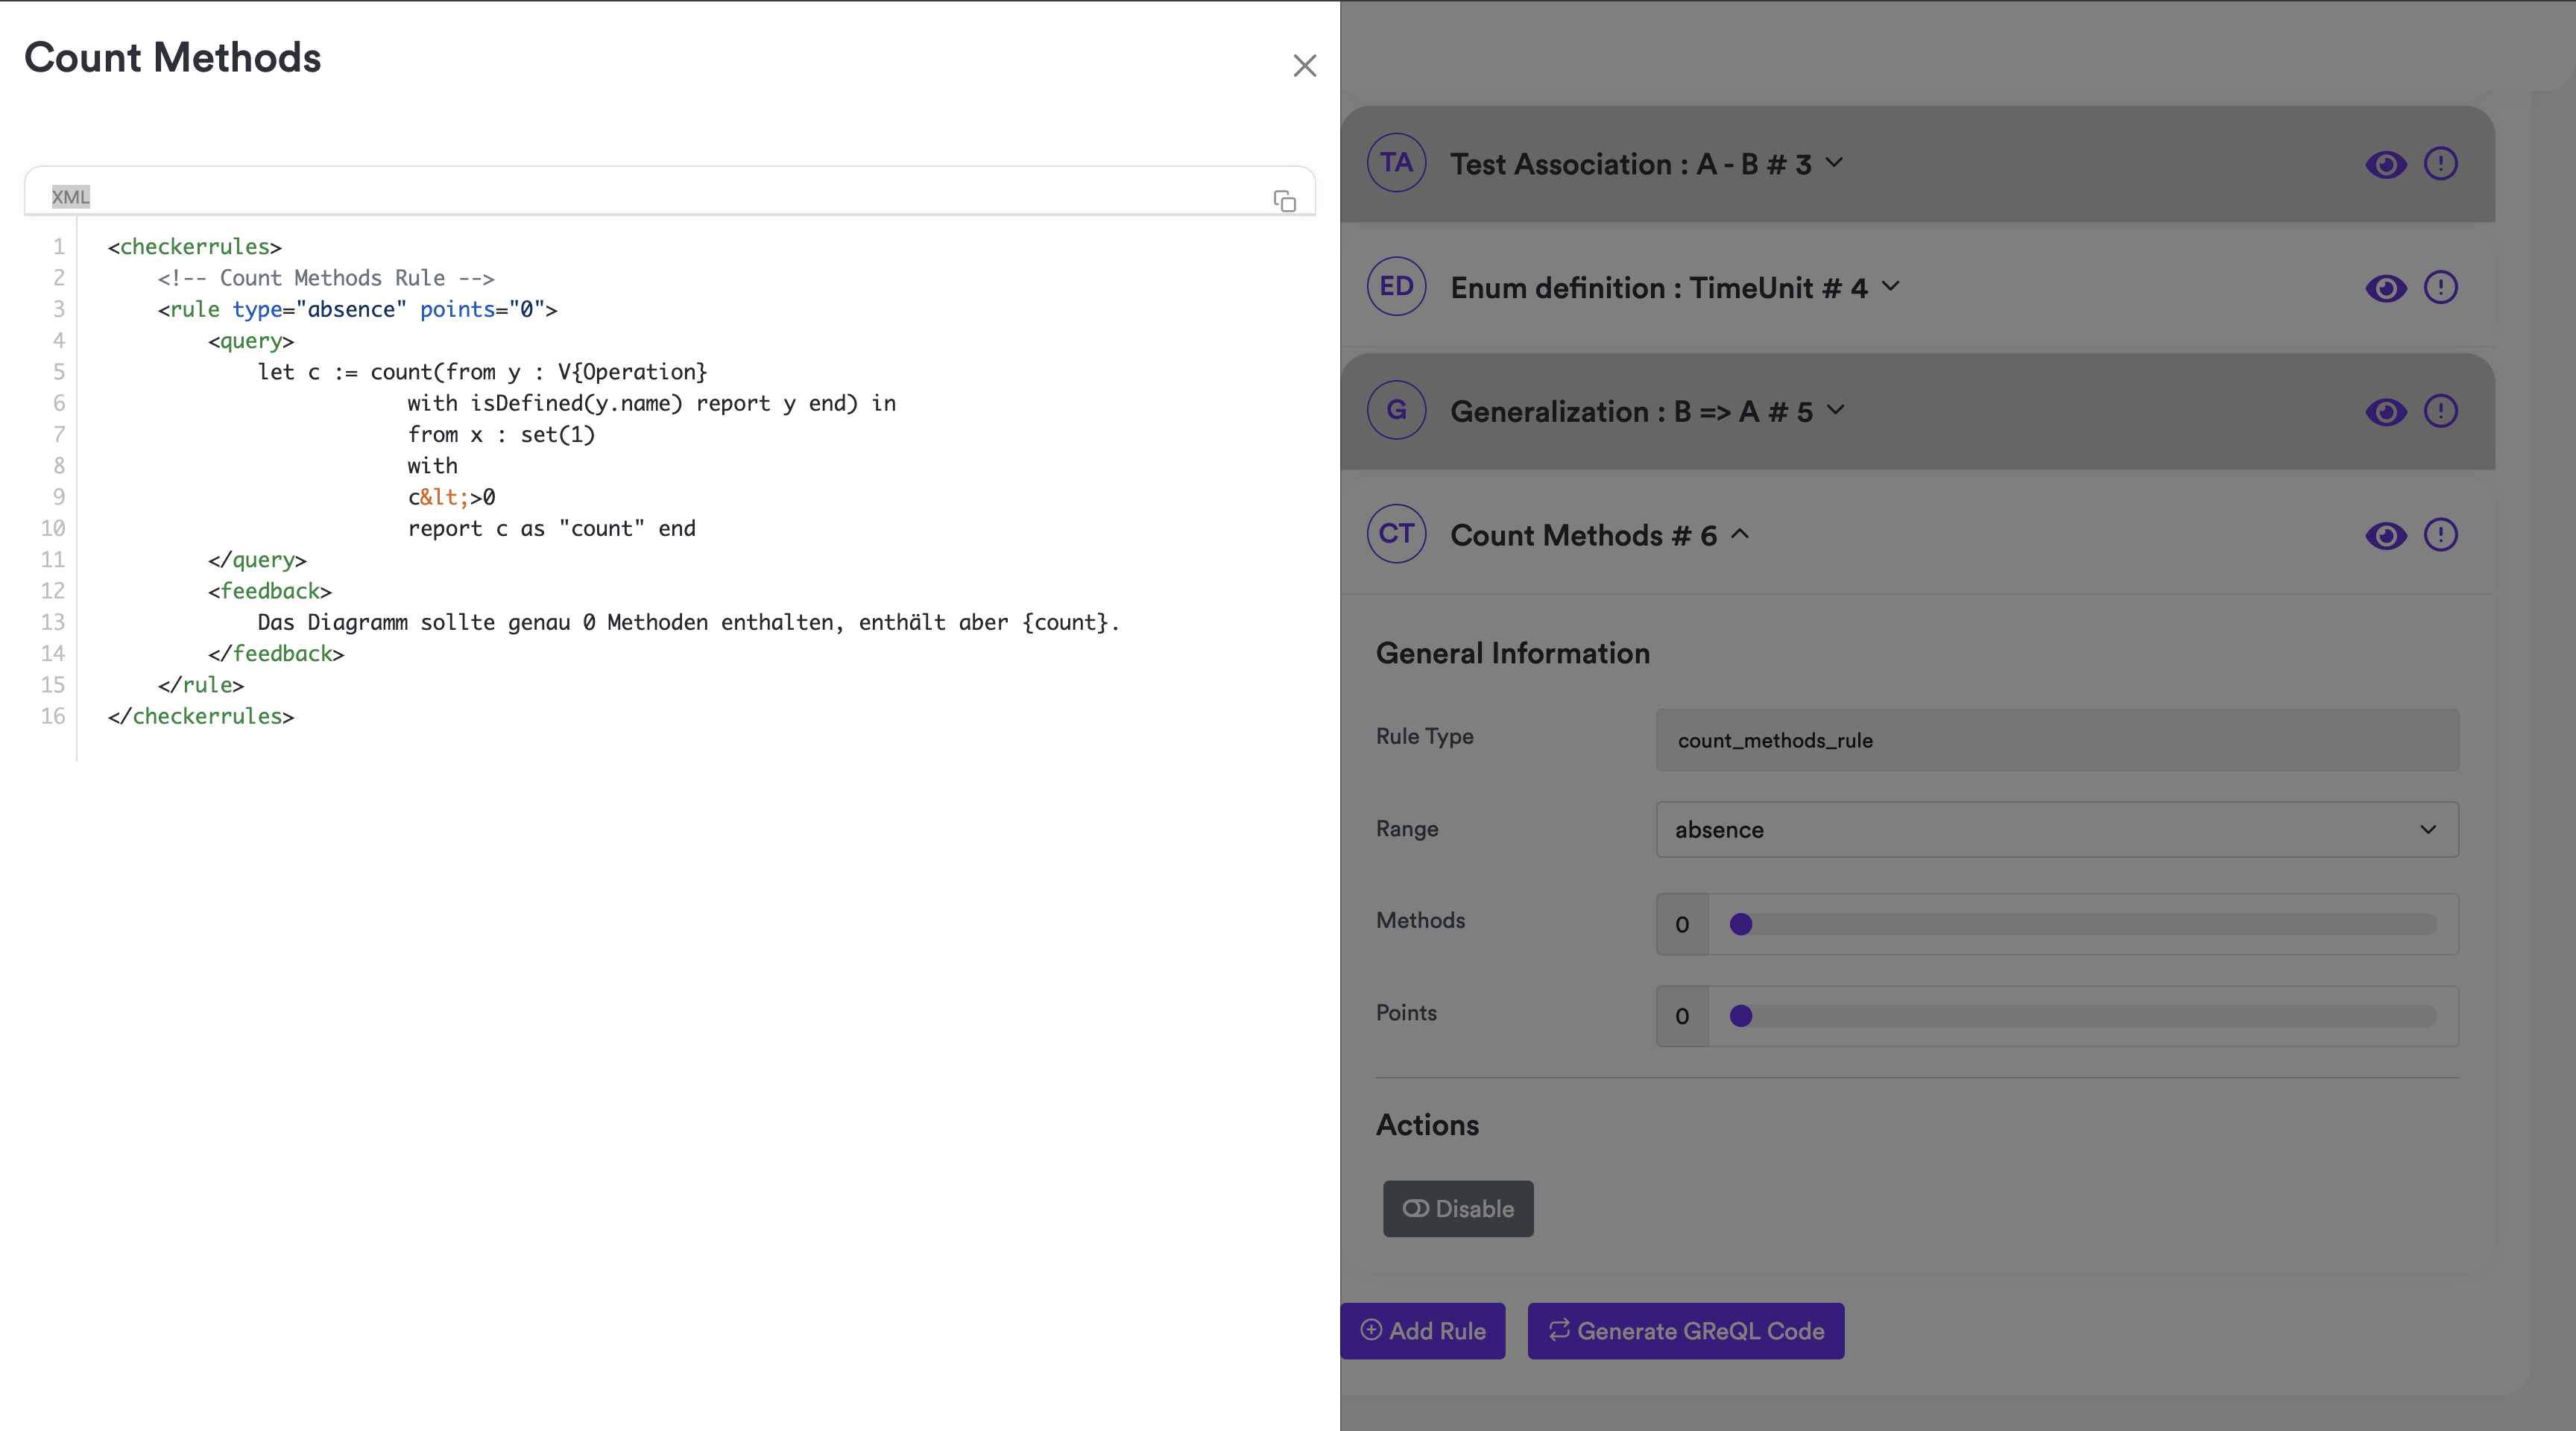
\includegraphics[width=16cm]{images/features-2n3}
    \caption{Feature 2 und 3}
    \medskip
    \small
    Auf der linken Seite des Bildes ist der GReQL-Code für die Regel ``Count Methods'' zu sehen. Um dieses Canvas
    anzuzeigen, kann man auf die Schaltfläche in Form eines Auges neben dem Titel der Regel klicken. Auf der linken
    Seite sind mehrere Regeln in Grau markiert, was bedeutet, dass sie deaktiviert sind. Diese werden daher bei der
    vollständigen Generierung des GReQL-Codes ignoriert.
    \label{fig:feat2n3}
\end{figure}

\subsection{Feature 4: Kombinierte Regeln}

Die erste Version des GReQL Converters war zweifellos sehr nützlich, da er die Erstellung einer großen Menge von Regeln
allein aus einem PlantText-Code ermöglichte. Allerdings blieb seine Nützlichkeit auf die Generierung einfacher und
größtenteils generischer Regeln beschränkt. Diese Einschränkung wurde vom Dr. Michael Striewe während seines Interviews
aufgezeigt, als er den Wunsch äußerte, komplexere Regeln aus annotiertem PlantText-Code zu generieren. Ein praktisches
Beispiel hierfür wäre zum Beispiel eine Klasse ``Bibliothek'', die ein oder mehrere Objekte der Klasse ``Buch'' enthält.
Diese einfache Darstellung kann auf verschiedene Arten modelliert werden, sei es durch das Hinzufügen von ``Buch'' als
Attribut zur Klasse ``Bibliothek``, durch Aggregation, Komposition oder einfache Beziehung. Die Einschränkung der ersten
Version des GReQL Converters bestand darin, dass er keine Möglichkeit bot, Regeln zu kombinieren, um verschiedene, aber
alle korrekte Antworten zu ermöglichen.

Um dieses Problem zu lösen, wurde die Entwicklung der Funktion zur Kombination von Regeln vorangetrieben. Diese Funktion
zielt darauf ab, eine gewisse Flexibilität zu bieten und Lehrkräften die Definition von deutlich komplexeren Regeln zu
ermöglichen. Damit können Variationen der Antworten definiert werden, die alle korrekt sein können. Um die
Funktionsweise dieser Funktionalität zu veranschaulichen, ist es sinnvoll, dies anhand eines Beispiels zu erläutern.
Angenommen, ein Lehrer möchte überprüfen, ob ein Schüler die richtige Beziehung zwischen der Klasse ``Bibliothek'' und
der Klasse ``Buch'' korrekt verwendet hat (siehe Abbildung~\ref{fig:combined}). Es gibt jedoch mehrere Möglichkeiten, wie diese
Beziehung konzipiert werden kann, wie zuvor erwähnt. Um GReQL-Code für diesen speziellen Fall zu generieren, wurde das
Annotationsystem erweitert. Durch das Stichwort ``combineID'' können Kombinationen mehrerer Regeln mit derselben
Kennung erstellt werden. Dies ermöglicht schließlich die Generierung von GReQL-Code (siehe Code~\ref{lst:combined}), der eine der
drei Bedingungen überprüft. Wenn eine dieser Bedingungen erfüllt ist, erhält der Schüler die Punkte. Details zu
diesem Annotationsystem finden sich in der Dokumentation des GReQL Converters.

\begin{figure}[h]
    \centering
    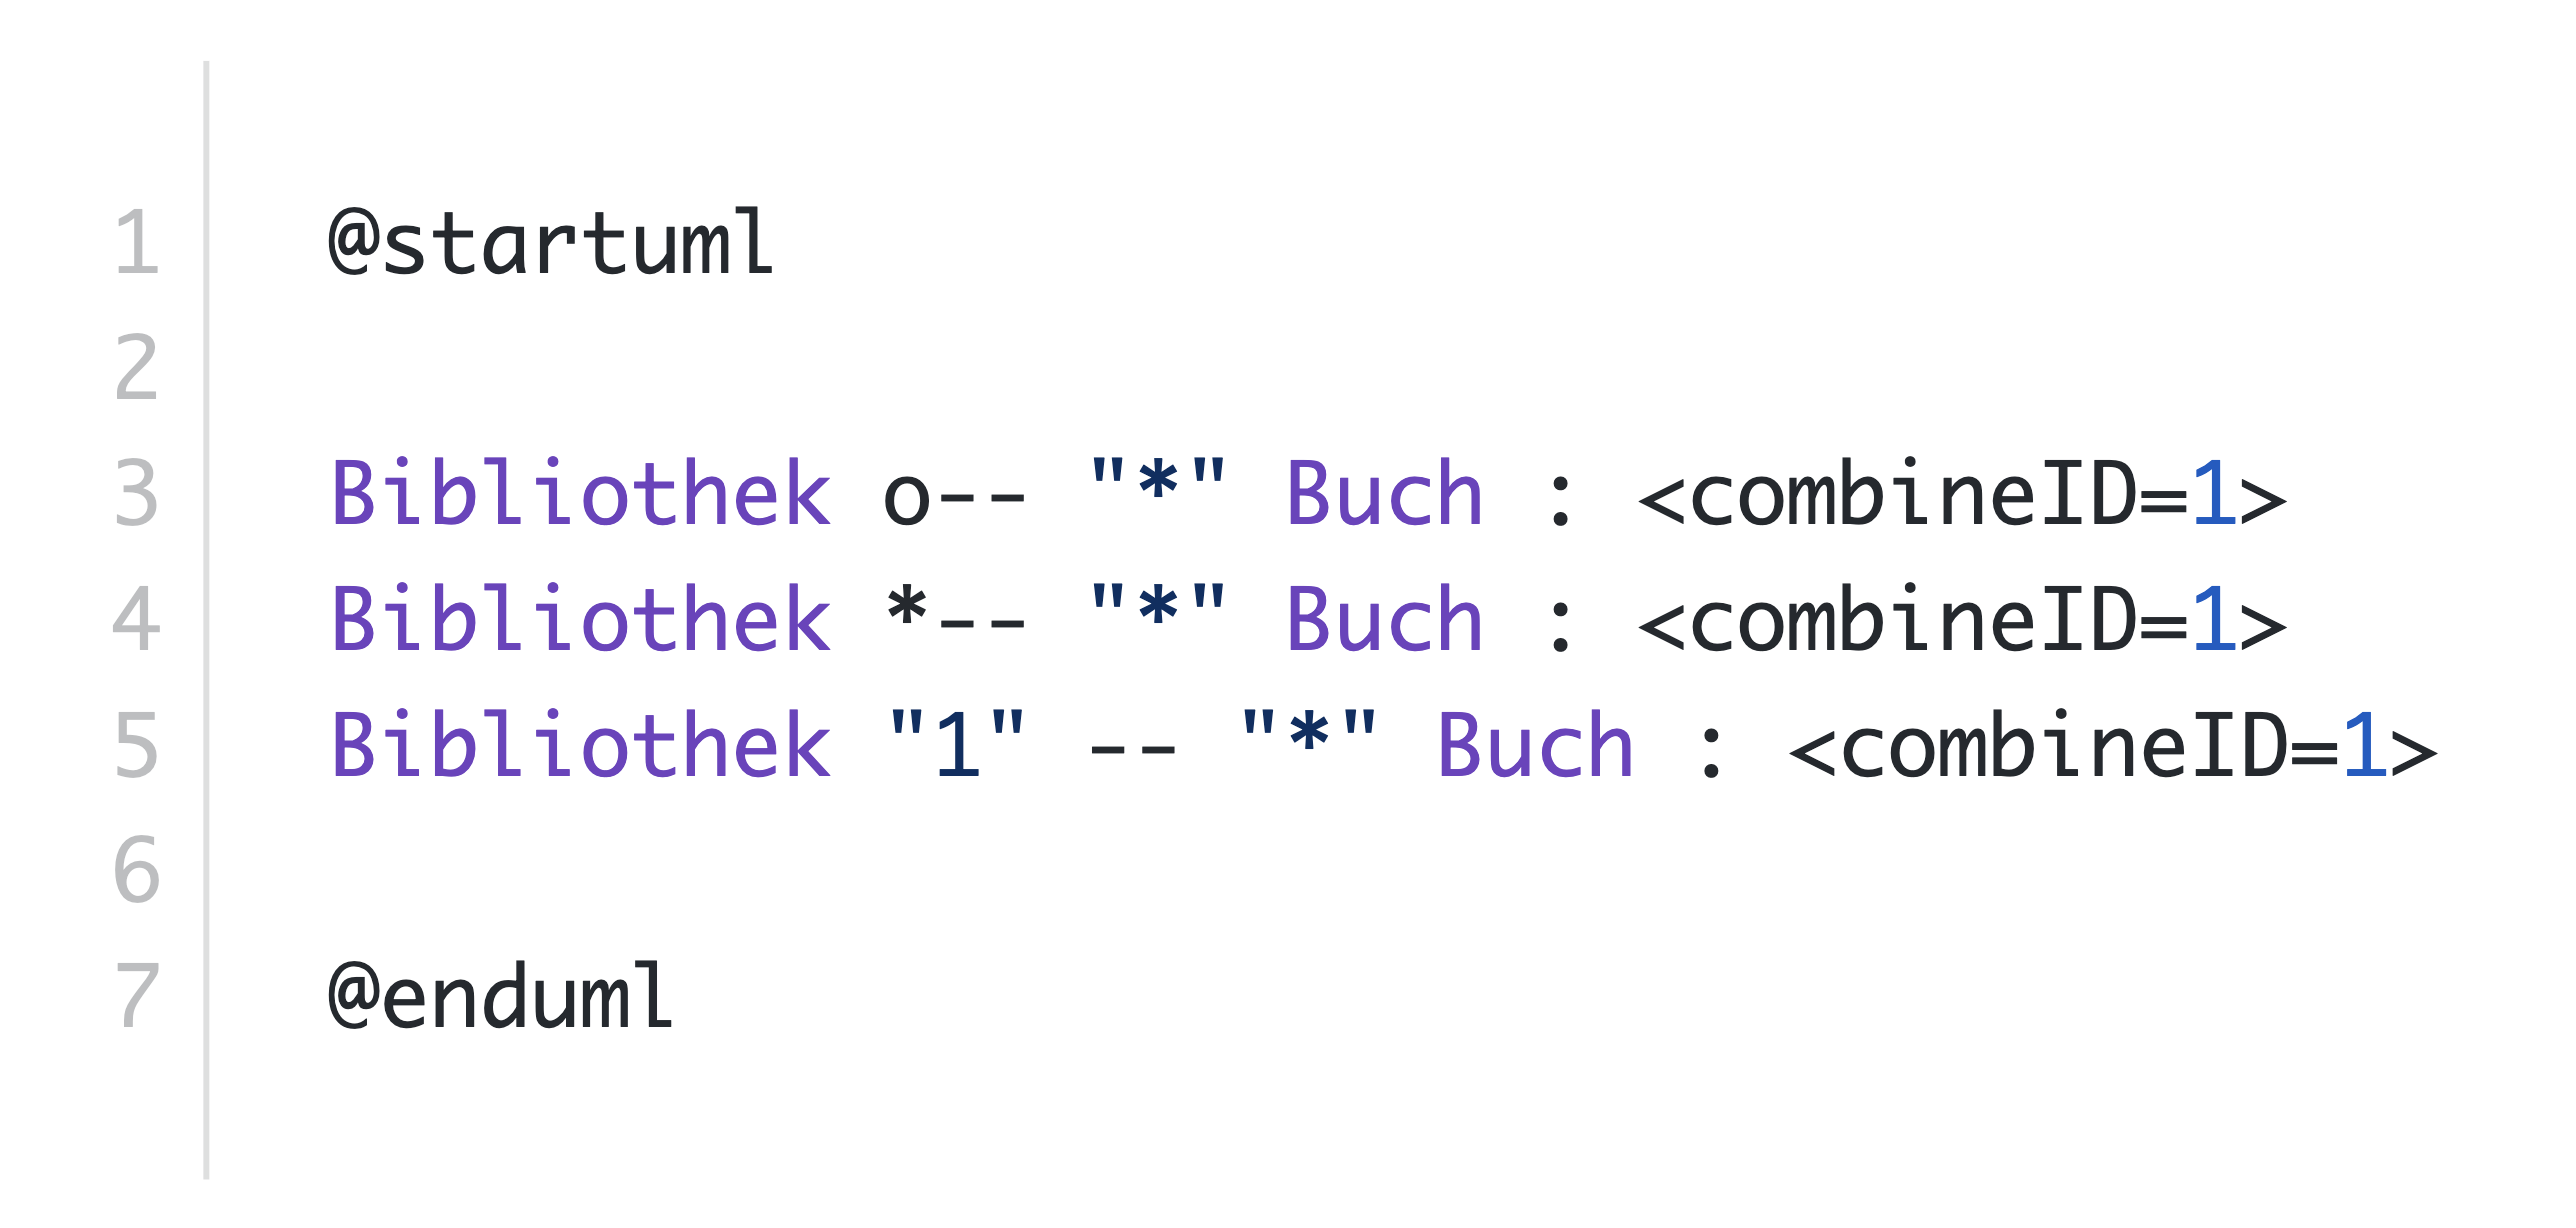
\includegraphics[width=16cm]{images/combined}
    \caption{Kombinierte Regeln}
    \label{fig:combined}
\end{figure}


\begin{lstlisting}[!h, caption={Ausschnitt aus dem GReQL-Code, der nach der Konvertierung erhalten wurde}, label={lst:combined}, language=xml]
<checkerrules>
    <!-- Combined  Rule -->

    <rule type="presence" points="0">

        <!-- Aggregation SubRule -->
        <query>
            from x, y : V{Class}, p: V{Property},
            a,b: V{LiteralString}
                with
                isDefined(x.name) and
                stringLevenshteinDistance(x.name,
                "Bibliothek")&lt;3 and
                isDefined(y.name) and
                stringLevenshteinDistance(y.name,
                "Buch")&lt;3 and
                isDefined(p.aggregation) and
                p.aggregation="shared" and
                x --> V{Property} -->
                V{Association} --> p &lt;-- y and
                isDefined(a.value) and
                a.value="*"  and
                isDefined(b.value) and
                b.value="*"  and
                x --> V{Property} --> a and
                x --> V{Property} --> b
                report 1 end
        </query>

        <!-- Composition SubRule -->
        <query>
            from x, y : V{Class}, p: V{Property},
            a,b: V{LiteralString}
                with
                isDefined(x.name) and
                stringLevenshteinDistance(x.name,
                "Bibliothek")&lt;3 and
                isDefined(y.name) and
                stringLevenshteinDistance(y.name,
                "Buch")&lt;3 and
                isDefined(p.aggregation) and
                p.aggregation="composite" and
                x --> V{Property} -->
                V{Association} --> p &lt;-- y and
                isDefined(a.value) and
                a.value="*"  and
                isDefined(b.value) and
                b.value="*"  and
                x --> V{Property} --> a and
                x --> V{Property} --> b
                report 1 end
        </query>

        <!-- Simple Association SubRule -->
        <query>
            from x,y : V{Class}, ass : V{Association},
            a,b,c,d  : V{LiteralString}
                with
                isDefined(x.name) and
                stringLevenshteinDistance(x.name,
                "Bibliothek")&lt;3 and
                isDefined(y.name) and
                stringLevenshteinDistance(y.name,
                "Buch")&lt;3 and
                isDefined(a.value) and
                a.value="*"  and
                isDefined(b.value) and
                b.value="*"  and
                x --> V{Property} --> a and
                x --> V{Property} --> b and
                isDefined(c.value) and
                c.value="1"  and
                isDefined(d.value) and
                d.value="1"  and
                y --> V{Property} --> c and
                y --> V{Property} --> d and
                x --> V{Property} --> ass
                &lt;-- V{Property} &lt;-- y
                report 1 end
        </query>
        <feedback>
            ... i need a feedback please 😊.
        </feedback>
    </rule>
</checkerrules>
\end{lstlisting}

\section{Zusammenfassung der Evaluation}

Abschließend bietet die Analyse und Bewertung des GReQL Converters einen detaillierten Einblick in die Wirksamkeit und
Potenziale dieses Tools. Die erörterten Verbesserungsvorschläge sowie die ermittelten Stärken und Schwächen legen den
Grundstein für zukünftige Entwicklungen und zeigen auf, wie dieses Instrument im Bildungsumfeld und darüber hinaus noch
effektiver genutzt werden könnte. Die Bewertung des Tools, getragen von den Erwartungen, dem Nutzen und den
Erkenntnissen aus den Anwendererfahrungen, bildet eine solide Grundlage für weiterführende Studien und Implementierungen
zur Steigerung seiner Funktionalitäten und Anwenderfreundlichkeit. Diese umfassende Bewertung legt den Fokus auf die
kontinuierliche Weiterentwicklung und Optimierung des GReQL Converters, um seinen Wert und seine Wirksamkeit für
zukünftige Anwendungen zu maximieren.

	\chapter{Diskussion}

Dieses Kapitel wird in mehrere Abschnitte unterteilt sein. Zunächst wird eine Interpretation der Ergebnisse der
Evaluation vorgenommen, um fundierte Schlussfolgerungen zu ziehen. Anschließend wird eine eingehende Diskussion über
die verschiedenen Herausforderungen geführt, die im Laufe des Entwicklungsprozesses des Tools bewältigt wurden.
Abschließend wird eine umfassende Untersuchung durchgeführt, um die verschiedenen Möglichkeiten zur Verbesserung des
GReQL Converters zu erörtern und sein fortwährendes Potenzial zu bewerten. Diese thematische Struktur zielt darauf ab,
eine ganzheitliche und gründliche Analyse der Leistung, der Herausforderungen und der Verbesserungsaussichten im
Zusammenhang mit diesem Tool bereitzustellen.

\section{Interpretation der Evaluationsergebnisse}


Die Interviews ergaben überwiegend positive Ergebnisse. Der GReQL Converter stellt ein innovatives Tool dar, das als
erstes seiner Art die Generierung von GReQL-Code ermöglicht, um Klassendiagramme zu bewerten. Alle Befragten äußerten
sich äußerst positiv über die Nützlichkeit des GReQL Converters und betonten dessen Potenzial, Lehrern erheblich Zeit
beim Verfassen von GReQL-Code zu sparen. Sie sind außerdem bereit, das Tool ihren Kollegen zu empfehlen, die bereits
Erfahrung mit GReQL-Code für die Klassendiagrammbewertung haben.

Die grafische Benutzeroberfläche und die Nutzererfahrung stießen bei den meisten Befragten auf Zustimmung.
Dennoch wurde auf verschiedene Bereiche hingewiesen, die noch verbessert werden könnten, um das Tool weiter zu
optimieren. Obwohl der GReQL Converter die Generierung generischer Regeln stark erleichtert, stellten die Interviews
fest, dass bei zunehmender Komplexität manuelle Eingriffe erforderlich sind. Es wurde betont, dass fortlaufende
Verbesserungen an dem Tool dazu beitragen könnten, den Bedarf an solchen manuellen Interventionen im Laufe der Zeit zu
verringern. Es ist jedoch wichtig zu beachten, dass der GReQL Converter nicht darauf abzielt, die menschliche
Intervention zu ersetzen. Stattdessen sollte er als unterstützendes Instrument für Lehrkräfte betrachtet werden.


\section{Herausforderungen während des Entwicklungsprozesses}

Im Verlauf des Entwicklungsprozesses manifestierten sich verschiedene herausfordernde Sachverhalte, die eine gezielte
Entwicklungsdynamik bedingten. Dies wiederum zwang die Notwendigkeit zur Implementierung spezifischer Beschränkungen
oder die Abkehr von bestimmten funktionalen Aspekten.

\subsubsection{PlantText Parser}

Bezüglich des PlantText Parsers sind gewisse Limitationen zu konstatieren. Er ist nicht in der Lage, statische
Attribute, statische Methoden und statische Klassen zu erfassen. Indessen fand rasch eine Lösung in Form eines
Kompromisses Anklang, indem dem Anwender ermöglicht wird, diese Modifikationen manuell im Rahmen des Regel-Editors
vorzunehmen.

\subsubsection{GReQL Engine Optimizer}

Der GReQL Engine Optimizer  verfügt über einen Algorithmus zur Optimierung von Abfragen, um deren Ausführung zu
erleichtern und mögliche Probleme wie die Verwendung undefinierter Variablen, welche eine Abfrage fehlerhaft machen
könnten, zu umgehen. Nichtsdestoweniger kann dieser Optimierer zuweilen Unklarheit in der Abfrageausführung stiften.
Es besteht die Möglichkeit, dass eine Abfrage verfasst wird, die auf den ersten Blick in vollkommen korrektem Einklang
erscheint, jedoch bei der Ausführung vom Optimierer in einer Art und Weise modifiziert wird, welche die Abfrage invalide
werden lässt (Wie es bei einigen Regeln im WIKI der Fall ist~\cite{GReQL-wiki}). Daraus resultiert, dass die GReQL Engine
Fehlermeldungen retourniert. Zur Bewältigung dieser Thematik waren eigens maßgeschneiderte Abfragen erforderlich, welche
verschiedene Prüfungen vor der Ausführung durchführen. In dieser Hinsicht erweist sich die Verwendung des GReQL
Converters als vorteilhaft, indem er ausschließlich valide Abfragen zur Optimierung generiert und dem Nutzer die
Frustration erspart, scheinbar korrekte, aber nicht funktionierende Abfragen manuell zu konzipieren.


\subsubsection{Beschränkung auf BOUML}

Der Kern des GReQL Converters liegt in der Erstellung und Definition von Vorlagen, die für jede Regel festgelegt wurden.
Zur Herstellung dieser Vorlagen war es erforderlich, zunächst ein Diagramm, welches die jeweilige Regel in Anspruch
nimmt, mittels der Software BOUML zu modellieren. Anschließend erfolgte die grafische Darstellung mithilfe des GReQL
Engine, um abschließend die Regel aus der grafischen Darstellung abzuleiten. Diese Vorgehensweise impliziert, dass die
Mehrzahl der in Gebrauch genommenen Regeln ihren Ursprung in einer bildlichen Repräsentation eines Diagramms haben,
welches mithilfe von BOUML erstellt wurde. Dies stellt ein substantielles Problem dar, da die XMI-Repräsentationen der
Diagramme abhängig vom verwendeten Tool variieren. Als Beispiel generiert der Enterprise Architect offensichtlich eine
XMI-Datei, die sich von derjenigen generiert durch BOUML zu unterscheiden scheint. Dies hätte zur Konsequenz, dass die
Mehrzahl der durch den GReQL Converter generierten Regeln ungültig würde, sofern das zu beurteilende Diagramm mittels
eines alternativen Tools geschaffen wurde. Das bedeutet, dass die Auswahl des Tools, das für die Generierung der
Lösungen zur Beurteilung eingesetzt wird, von entscheidender Relevanz ist, was wiederum den GReQL Converter auf eine
spezifische Werkzeugauswahl oder auf die Nutzung von BOUML für die Gestaltung der zu beurteilenden Diagramme beschränkt.

\subsubsection{Primitive Datentypen}

Im Zusammenhang mit den von BOUML generierten Diagrammen ist zu berücksichtigen, dass sie einem ausgewiesenen Standard
entsprechen, nämlich dem UML-Standard 2.3~\cite{OMG_UML_23_Infrastructure}, der von BOUML in Gebrauch genommen wird.
Dieser Standard erkennt jedoch lediglich vier primitive Datentypen, nämlich int, bool, string und
UnlimitedNatural~\cite{OMG_UML_23_Infrastructure}. Diese Beschränkung führt dazu, dass Typen, die im Grundsatz als
primitiv erachtet werden könnten, wie double, float, char und dergleichen, schlichtweg nicht berücksichtigt werden.
Dieses Problem hat zur Folge, dass Typen in GReQL-Abfragen nicht überprüft werden können, sofern sie nicht den Kriterien
des UML 2.3-Standards genügen. In praktischer Konsequenz mussten gewisse Funktionen aufgegeben werden, etwa die
Überprüfung des Rückgabetyps einer Methode oder des Typs einer Variablen (sofern diese nicht gemäß UML 2.3 als primitiv
gelten), da die Repräsentation, die durch die GReQL Engine erzeugt wird (basierend auf dem XMI von BOUML), diese Typen
nicht erkennt und daher nicht darstellen kann. Infolgedessen können derlei Abfragen nicht ausgeführt werden.
\\~\\
Diese genannten Beschränkungen stellen zweifelsohne vielversprechende Ansatzpunkte für eine substantielle Verbesserung
des GReQL Converters dar. Daher wird in dem folgenden Abschnitt eine Diskussion darüber eingeleitet, wie der GReQL
Converter möglicherweise verbessert werden kann, um einige dieser inhärenten Einschränkungen zu überwinden.


\section{Potenziale für Weiterentwicklungen}

Der GReQL Converter, obwohl er vielversprechend ist, verwehrt sich der Illusion der Vollkommenheit. In diversen Domänen
sind signifikante Verbesserungen realisierbar, um seine Effektivität bei der Bewältigung spezifischer Herausforderungen
zu optimieren.

\subsection{Hinzufügen neuer Regeln}

Eine solche Möglichkeit zur Verbesserung manifestiert sich in der Erweiterung des Regelkatalogs. Obwohl die Entwicklung
des GReQL Converters bereits eine umfassende Berücksichtigung der Regeln, die der Modellierung von UML-Klassendiagrammen
zugrunde liegen, einschloss, bleiben einige subtile Nuancen unvollständig berücksichtigt. Zum Beispiel wurden keine
Regeln für Assoziationen mit spezifischer Richtung oder für nicht-ausgerichtete Beziehungen integriert. Während die
Assoziation zwischen zwei Klassen betrachtet wird, sofern eine Beziehung zwischen ihnen besteht, erfolgt keine explizite
Erfassung der Ausrichtung dieser Assoziation. Ebenso bleiben die mit Assoziationen verknüpften Rollennamen
unberücksichtigt. Diese und andere Feinheiten könnten zukünftige Erweiterungen des GReQL Converters sein, um das Tool
in Bezug auf die Generierung präziserer GReQL-Regeln zu bereichern.


\subsection{Erweiterung bestehender Regeln}

Eine Vielzahl von Regeln könnte von Verbesserungen profitieren, um eine größere Bandbreite von Designvarianten zu
unterstützen und kompatibler zu werden. Um dieses Ziel zu erreichen, ist es unerlässlich, den GReQL Converter an einer
beträchtlichen Anzahl von Diagrammen zu testen, um seine Grenzen und Einschränkungen zu identifizieren und umfassend
anzugehen. Durch eine breite Testbasis können potenzielle Schwachstellen erkannt und verbessert werden, um eine
robustere und flexiblere Anwendung des Tools zu gewährleisten.


\subsection{Erweiterung der Kompatibilität des GReQL Converter}

Wie zuvor erwähnt, ist der von GReQL Converter generierte GReQL-Code derzeit zu 100\% kompatibel mit Lösungsdiagrammen,
die mit BOUML erstellt wurden. Der GReQL Converter wurde jedoch mit Blick auf die Erweiterbarkeit zu anderen
Technologien entwickelt, die die Modellierung von UML-Diagrammen und die Generierung von XMI-Dateien ermöglichen. Die
Erweiterung auf andere Diagramm-Modellierungstools sollte hauptsächlich das Hinzufügen von regelbasierten Vorlagen für
diese Tools und die Möglichkeit zur Auswahl des bevorzugten Tools über die grafische Benutzeroberfläche des GReQL
Converter einschließen. Glücklicherweise sollte diese Aufgabe nicht besonders komplex sein.


\subsection{Erweiterung des PlantText-Syntaxparsers zur Erkennung von Syntaxfehlern}

Während des Interviews mit Dr. Michael Striewe wurde ein Verhalten bemerkt. Als er seinen PlantText-Code auf die
Plattform kopierte, konnten nur die Klassendefinitionen Regeln (``Class Definition'') generiert werden, und die
Assoziationsregeln wurden nicht erkannt. Dies lag daran, dass die Klassennamen in den Assoziationen in
Anführungszeichen standen, was der Parser nicht erkennen konnte. Dieses Problem lässt sich dadurch erklären, dass der
Parser solche Ausdrücke nicht als Fehler erkennt. Es gibt mehrere Arten von gültigem PlantText-Code, der jedoch nicht
zwangsläufig vom Parser verarbeitet werden kann. Aus diesem Grund sollte man sich an die Dokumentation halten, um die
Regeln zu schreiben, und auf der Entwicklungsseite einen Weg finden, diese Fehler zu identifizieren und insbesondere den
Benutzer darauf aufmerksam zu machen, dass etwas nicht wie erwartet funktioniert. Das gilt auch für den Fehler, den er
bezüglich des Enums erwähnt hat, der eine spezifische Syntax im GReQL Converter erfordert.


Der PlantText-Parser ist ein Open-Source-Projekt, was bedeutet, dass der Quellcode für jeden zugänglich,
modifizierbar und verteilbar ist. Es ist also möglich, direkt auf der Parser-Ebene Änderungen vorzunehmen, um Funktionen
hinzuzufügen und damit seine Fähigkeiten zu erweitern.


\subsection{Erweiterung auf andere UML-Diagrammtypen}

Im Rahmen dieser Masterarbeit wurde der GReQL Converter auf die Generierung von GReQL-Code für UML-Klassendiagramme
spezialisiert. Während der Entwicklung wurde jedoch berücksichtigt, dass das Tool erweitert werden kann, um auch andere
Arten von Diagrammen wie Aktivitäts-, Sequenz- oder sogar Use-Case-Diagramme zu unterstützen. Es ist bereits möglich,
mithilfe von GReQL Code zu schreiben, um diese genannten Diagrammtypen zu evaluieren. Zusätzlich sind diese Diagramme
mithilfe von PlantUML modellierbar. Folglich könnte der GReQL Converter tatsächlich erweitert werden, um Code für
verschiedene Arten von Diagrammen zu generieren. Es wäre also ein Ansatz zur Verbesserung des GReQL Converters, nicht
nur auf Klassendiagramme beschränkt zu sein, sondern auch andere Diagrammtypen zu unterstützen. Dies würde das Tool
vielseitiger machen und seine Anwendungsfälle deutlich erweitern.

\section{Erweiterbarkeit des GReQL-Converters}

In den vorherigen Abschnitten wurde erläutert, dass der GReQL Converter so entwickelt wurde, dass eine einfache 
Erweiterung möglich ist. Dies ermöglicht zukünftigen Entwicklern, die Funktionalität des Tools zu erweitern, ohne 
mehrere Teile des Codes ändern zu müssen, was zu Fehlern führen könnte. Dieser Abschnitt präsentiert die 
Gesamtarchitektur des Datentransits im GReQL Converter sowie verschiedene Möglichkeiten zur Erweiterung des Tools.

\subsection{Datentransit im GReQL-Converter}

Der Prozess zur Generierung des GReQL-Codes aus dem GReQL Converter durchläuft mehrere Schritte, die bereits im
Implementierungskapitel beschrieben wurden. Diese Sektion bietet detaillierte Einblicke, die wichtig sind, um zu
verstehen, wie die Funktionalitäten des Tools erweitert werden können. Dieser Prozess wird durch
Abbildung~\ref{fig:transit} veranschaulicht, die die verschiedenen Schritte des Datentransits zeigt.


Es beginnt zunächst mit dem PlantText-Code der Lehrkraft, der an den PlantText-Parser gesendet wird, der auf einem
Node.js-Server läuft. Der Parser gibt ein JSON-Objekt zurück, das Informationen über die UML-Entitäten sowie deren
Beziehungen enthält (siehe Code~\ref{lst:parsed-json}). Nach diesem Schritt wird dieses JSON vom ``Class Converter''
verarbeitet. Der Class Converter nutzt das JSON des Parsers und enthält Methoden zur Identifizierung von Entitäten und
Beziehungen, wodurch Regeln für jede Entität und Beziehung generiert werden. Die Art und Weise dieser
Identifizierung wird im Implementierungskapitel beschrieben (siehe Code~\ref{lst:condition-check}).


Der Class Converter verwendet die ``Class Rules Definition'' zur Generierung der Regeln. Die Class Rules Definition ist
eine Art Enum, die als Konfigurationsdatei betrachtet werden kann (siehe Code~\ref{lst:rules_def}). Sie enthält alle
Definitionen für jedes Objekt des Regeltyps. In dieser Datei ist es möglich, eine neue Regel und ihre Attribute zu
definieren. Mithilfe dieser Datei kann der Class Converter Regeln basierend auf dem JSON des Parsers generieren.
Die Verwendung der Class Rules Definition spielt eine entscheidende Rolle im GReQL Converter, da viele andere
Komponenten von dieser Klasse abhängig sind.


Es wäre möglich gewesen, diese Regelobjekte direkt im Class Converter zu generieren, ohne die Class Rules Definition und
unabhängig von anderen Anwendungskomponenten zu nutzen. Diese Objekte wären dann fest codiert gewesen, was eine
schlechte Praxis darstellt. Dies hätte jedoch den Prozess des Hinzufügens und der Anpassung von Regeln in anderen
Komponenten (die in Kürze erwähnt werden) unnötig komplex gemacht. Dies hätte von zukünftigen Entwicklern verlangt,
Änderungen an mehreren Stellen vorzunehmen.


Jedoch ermöglicht die Verwendung der Class Rules Definitions eine harmonisierte Regelgenerierung. Es wäre lediglich
erforderlich, diese Datei zu ändern und entsprechende Zuordnungen in den sie nutzenden Dateien hinzuzufügen oder zu
entfernen, um eine neue Regel hinzuzufügen oder zu entfernen. Die Regeln, die vom Lehrer geändert werden können,
erfordern eine grafische Darstellung. Diese grafische Darstellung wird durch Vue.js-Klassen realisiert, die Regeln
darstellen. Diese Vue.js-Klassen ermöglichen es dem Lehrer, die generierten Regelobjekte auf der grafischen
Benutzeroberfläche zu ändern (siehe Abbildung~\ref{fig:extracted_rules}). Diese Vue.js-Klassen nutzen natürlich die
Class Rules Definitions, um die Regelobjekte ihren verschiedenen Platzhaltern zuzuordnen.

Nach diesen Generierungs- und Änderungsschritten wird eine Liste mit allen Regelobjekten erstellt. Diese Liste wird
dann an den ``Class GReQL Rules Generator'' gesendet. Der Class GReQL Rules Generator generiert basierend auf jeder
Regel den entsprechenden GReQL-Code. Für jedes Objekt in der Liste identifiziert er zunächst den Regeltyp und generiert
dann den entsprechenden GReQL-Code. Der Generierungsprozess wurde im Implementierungskapitel ausführlich beschrieben
(siehe Code~\ref{lst:class_def_xml}). Für jeden Regeltyp ist eine spezifische Methode für die Generierung des
GReQL-Codes verantwortlich.

Es wäre auch möglich gewesen, eine einzige Methode zu schreiben, die die gesamte Liste umwandeln könnte. Dies hätte
jedoch den Prozess der Regelgenerierung unnötig komplex gemacht. Es wäre für einen neuen Entwickler schwer gewesen, die
Funktionsweise der Methode zu verstehen und die Punkte zu identifizieren, an denen eine neue Regel hinzugefügt oder
eine bereits vorhandene geändert werden könnte. Der gewählte Ansatz erleichtert das Hinzufügen neuer Regeln. Diese
Vorgehensweise schafft eine Abstraktion, die die Trennung der Generierung verschiedener Regeltypen erleichtert und somit
die Entwicklererfahrung verbessert.

Am Ende dieses Prozesses wird der GReQL-Code erhalten, der von bestimmten Bibliotheken leicht modifiziert wird, um ihn
auf der Benutzeroberfläche darstellbar zu machen. Diese Sektion beschreibt den Datenverkehr in der Anwendung recht
abstrakt.

\begin{figure}[h!]
    \centering
    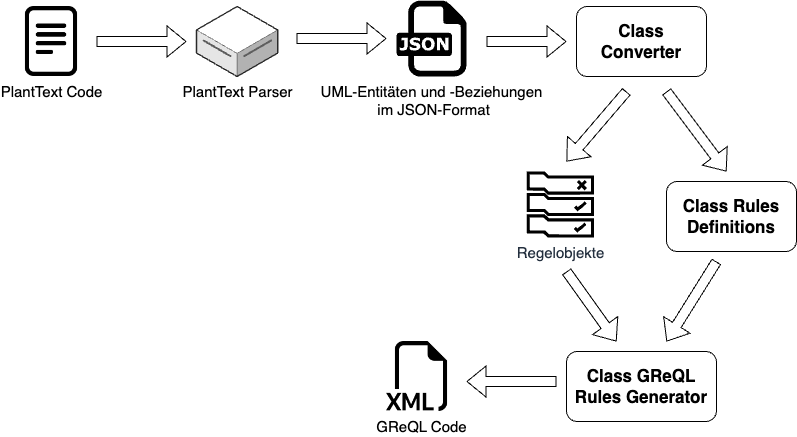
\includegraphics[width=12cm]{images/transit}
    \caption{Repräsentatives Schema des Datentransits im GReQL-Converter.}
    \label{fig:transit}
\end{figure}

\subsection{Prozess der Integration neuer Regeln}
write something here

\subsection{Prozess zur Erweiterung der Kompatibilität mit einer neuen Plattform}
write something here

\subsection{Prozess der Erweiterung um einen neuen Diagrammtypus}
write something here


\section{Zusammenfassung der Diskussion}

Die Entwicklung des GReQL Converters basierte auf der grundlegenden Überlegung, ein Tool zu schaffen, das sich
kontinuierlich weiterentwickeln kann. Dieser Aspekt fand sich in der Gestaltung des Codes wider, der gemäß etablierter
Designprinzipien und bewährter Praktiken verfasst wurde. Der Fokus lag darauf, kommenden Entwicklern, die an diesem Tool
arbeiten, eine klare Orientierung zu bieten und ihre Entwicklererfahrung erheblich zu verbessern, wie auch McConnell es
erwähnt~\cite{mcconnell2006software}. Diese strategische Herangehensweise zielt darauf ab, eine solide Grundlage zu
schaffen, die zukünftige Erweiterungen und Anpassungen erleichtert und einen nahtlosen Entwicklungsprozess für kommende
Versionen des GReQL Converters ermöglicht.

	\chapter{Zusammenfassung und Ausblick}
\section{Zusammenfassung}
\section{Ausblick}
	
	\printbibliography[heading=bibintoc]
	
	\appendix
	% !TeX root = main.tex

\chapter{Appendix}
\section{Einige Teile des Quellcode}
\subsection{Backend Quellcode}

\begin{lstlisting}[caption={Node/Express Backend Quelltext}, label={lst:bakcend}, language=javascript]
const express = require('express');
const bodyParser = require('body-parser');
const { parse } = require('plantuml-parser');
const cors = require('cors');
const app = express();
const port = 3000;
app.use(cors());
app.use(bodyParser.json());
app.post('/convert', (req, res) => {
  const code = req.body.code;
  try {
    const parsedCode = parse(code);
    if(parsedCode.length === 0)
       throw new Error('Failed to parse PlantUML code')

    res.json(parsedCode);
  } catch (error) {
    res.status(500)
.json({ error: 'Failed to parse PlantUML code' });
  }
});
app.listen(port, () => {
  console.log(`Server is running on port: ${port}`);
});
\end{lstlisting}


\subsection{Frontend Quellcode}
\subsubsection{Rules Definition JSON}
\begin{lstlisting}[caption={Rules Definition JSON}, label={lst:rules_def}, language=javascript]
export default {
    RULE_TYPE: {
        // CLASS & INTERFACE
        'defined_class': 'defined_class_rule',
        'defined_enum': 'defined_enum_rule',

        // GENERALIZATION & SPECIALIZATION
        'generalization': 'generalization_rule',

        // RELATIONSHIPS
        'simple_association': 'simple_association_rule',
        'composition': 'composition_rule',
        'aggregation': 'aggregation_rule',

        // ASSOCIATION CLASS
        'association_class': 'association_class_rule',

        // OPTIONAL
        'nomination_consistency': 'nomination
_consistency_rule',
        'test_association': 'test_association_rule',
        'count_methods': 'count_methods_rule',
        'count_attributes' : 'count_attributes_rule'

    },
    RULE_TYPE_JSON: {
        // CLASS & INTERFACE
        'defined_class_rule' : {
            rule_type: 'defined_class_rule',
            rule_name: 'Class definition',
            feedback: '... no feedback yet',
            points: 0,
            existence: 'presence',
            rule_specific: {
                class_name: "Car",
                abstract: false,
                interface: false,
                methods: [],
                attributes: [],
            }
        },
        // ENUM
        'defined_enum_rule' : {
            rule_type: 'defined_enum_rule',
            rule_name: 'Enum definition',
            feedback: '... no feedback',
            points: 0,
            existence: 'presence',
            rule_specific: {
                enum_class_name: "Car",
                attributes: [],
            }
        },
        // GENERALIZATION & SPECIALIZATION
        'generalization_rule' : {
            rule_type: "generalization_rule",
            rule_name: "Generalization",
            existence: "presence",
            points: 0,
            feedback: '... no feedback',
            rule_specific: {
                class_child: "Child",
                class_parent: "Parent",
                type: "inheritance" // implementation
            }
        },
        // RELATIONSHIPS
        'simple_association_rule': {
            rule_type: "simple_association_rule",
            rule_name: "Simple Association",
            existence: "presence",
            points: 0,
            feedback: "... no feedback",
            rule_specific: {
                class_A: "Class A",
                class_B: "Class B",
                A_multiplicity: "1",
                B_multiplicity: "1"
            }
        },
        'composition_rule' : {
            rule_type: "composition_rule",
            rule_name: "Composition",
            existence: "presence",
            points: 0,
            feedback: "... no feedback",
            rule_specific: {
                class_composite: "Composite",
                class_element: "Element",
                composite_multiplicity: "1",
                element_multiplicity: "*",
            }
        },
        'aggregation_rule' : {
            rule_type: "aggregation_rule",
            rule_name: "Aggregation",
            existence: "presence",
            points: 0,
            feedback: "... no feedback",
            rule_specific: {
                class_aggregate: "Aggregate",
                class_element: "Element",
                aggregate_multiplicity: "1",
                element_multiplicity: "*",
            }
        },
        // ASSOCIATION CLASS
        'association_class_rule' : {
            rule_type: "association_class_rule",
            rule_name: "Association Class",
            existence: "presence",
            points: 0,
            feedback: "Es muss eine Asso...",
            rule_specific: {
                class_A: "Class A",
                class_B: "Class B",
                class_C: "Class C"
            }
        },
        // OPTIONAL
        'nomination_consistency_rule' : {
            rule_type: "nomination_consistency_rule",
            rule_name: "Nomination Consistency",
        },
        'count_methods_rule' : {
            rule_type: "count_methods_rule",
            rule_name: "Count Methods",
            existence: 'absence',
            points: 0,
            rule_specific: {
                methods: 0,
            }
        },
        'count_attributes_rule' : {
            rule_type: "count_attributes_rule",
            rule_name: "Count Attributes",
            existence: 'absence',
            points: 0,
            rule_specific: {
                attributes: 0,
            }
        },
        'test_association_rule' : {
            rule_type: "test_association_rule",
            rule_name: "Test Association",
            existence: "absence",
            points: 0,
            rule_specific: {
                class_A: "Class A",
                class_B: "Class B",
            }
        },
    },
    METHODS_TYPE: {
        name: "public_method_name",
        return_type: "void",
        visibility: "public",
        arguments: "",
        points: 0,
        feedback: '... no feedback',
        is_static: false
    },
    ATTRIBUTE_TYPE: {
        name: "attribute_name",
        type: "string",
        visibility: "public",
        points: 0,
        feedback: '... no feedback',
        is_static: false
    },
    ENUM_ATTRIBUTE_TYPE: {
        name: "ENUM_ATTR",
        points: 0,
        feedback: '... no feedback',
    },
    EXISTENCE_TYPE: {
        'presence': 'presence',
        'absence' : 'absence'
    },
    GENERALIZATION_TYPE: {
        'inheritance': 'inheritance',
        'implementation': 'implementation'
    }
}
\end{lstlisting}
	
	\newpage
	% !TeX root = main.tex

\thispagestyle{empty}
\section*{Eidesstattliche Erklärung}
Hiermit versichere ich, dass ich die vorliegende Arbeit ohne Hilfe Dritter und nur mit den angegebenen Quellen und Hilfsmitteln angefertigt habe.
Ich habe alle Stellen, die ich aus den Quellen wörtlich oder inhaltlich entnommen habe, als solche kenntlich gemacht. Diese Arbeit hat in gleicher oder ähnlicher Form noch keiner Prüfungsbehörde vorgelegen.

\vspace{5em}

\begin{flushleft}
	\begin{tabular}{l}
		\hline \\
		\author, \location, den \date
	\end{tabular}
\end{flushleft}
 
\end{document}